\documentclass[12pt, a4paper]{report}
\usepackage{graphicx, array, amsthm, amssymb, amsmath, float, xcolor, thmtools, thmbox, geometry, listings, hyperref, tabularx, titling}
\usepackage[english]{babel}
\geometry{a4paper, left=2cm, right=2cm, top=2.5cm, bottom=2.5cm}

\title{Design Document}
\author{Christian Rossi \\ Kirolos Sharoubim}
\date{Academic Year 2023-2024}

\begin{document}

\begin{titlingpage} 
    \begin{center}
        
\includegraphics[height=5cm]{images/polimi.png}\\
        \vspace{4cm}
        \begin{huge} 
            \textbf{\thetitle} \\
        \end{huge}
        \vspace{0.3cm}
        \begin{Large}
            \textit{Software Engineering 2 \\ CodeKataBattle} \\
        \end{Large}
    \end{center}
    \vspace{6.9cm}
        \begin{center}      
            \textbf{Authors}    

            Christian Rossi - 10736464   

            Kirolos Sharoubim - 10719510
    \end{center}
\end{titlingpage}

\tableofcontents

\chapter{Introduction}
    \section{Purpose}
    This document aims to provide a comprehensive insight into the CodeKataBattle system outlined in the RASD.
    It delves into the system's architecture, elucidating on its components, their interactions, processes, and algorithms designed to meet RASD requirements. 
    Furthermore, it offers explicit instructions pertaining to the implementation, integration, and testing plan. 
    Geared towards developers, testers, and project managers, this document serves as a valuable reference for the system's implementation phase.

    \section{Scope}
    CodeKataBattle serves as a platform utilized by educators to engage students in coding Katas - challenges designed to be addressed using a programming language specified by the challenge organizers. 
    Educators possess the capability to establish a code Kata within a particular tournament, defining essential parameters such as the problem statement (inclusive of test cases), 
    the minimum and maximum number of students allowed per group, and the deadlines for both code Kata registration and solution submission.
    Following the tournament creation, students are empowered to create groups and commence their collaborative efforts on the solution, following a test-first approach. 
    As the ultimate deadline approaches, the system autonomously computes the final rankings, ultimately revealing the victorious participants.
    For a more comprehensive overview of the features accessible to end users, please consult the RASD. 
    The architecture of the S2B is structured into three physically separated layers, each installed on distinct tiers. 
    These layers are:
    \begin{enumerate}
        \item \textit{Presentation layer}: responsible for overseeing the presentation logic and handling all interactions with end users.
        \item \textit{Business logic layer}: manages the application functions provided, ensuring seamless operation and functionality.
        \item \textit{Data layer}: handles secure storage and facilitates access to data, ensuring the integrity and reliability of information.
    \end{enumerate}

    \section{Definitions, acronyms and abbreviations}
    \subsection{Definitions}
    \textbf{Code Kata}: adaptation of the concept of karate katas, where you repetitively refine a form, to the realm of software development, 
        fostering iterative practice and improvement. 
    \\
    \textbf{Test-first approach}:  software development process relies on the transformation of software requirements into test cases before 
        the software is completely developed, and it involves monitoring the entire software development by iteratively testing the software 
        against all these test cases.
    \subsection{Acronyms}
    \textbf{CKB}: CodeKataBattle 
    \\
    \textbf{CK}: Code Kata
    

    \section{Revision history}
    \textbf{Version 1.0} - Release - 04-01-2024


    \section{Reference documents}
    \textbf{Document 1} - Presentation about DD structure
    \\
    \textbf{Website 1} - http://codekata.com
    \\
    \textbf{Website 2} - https://en.wikipedia.org

    \section{Document structure}
    This document comprises seven sections:
    \begin{enumerate}
        \item \textit{Introduction}: this section furnishes an overview of the Design Document (DD), encompassing the project's scope, key term definitions, references to pertinent documents, and a brief outline of the design. 
        \item \textit{User interface design}: outlining the design of the user interface (UI) along with user experience (UX) flowcharts, this section provides a detailed perspective on how users will interact with the system. 
        \item \textit{Architectural design}: describing the high-level components and interactions within the system, this section includes a component view, deployment view, runtime view, and insights into selected architectural styles and patterns.
        \item \textit{Requirements traceability}: establishing a clear connection between the requirements specified in the Requirements and Specification Document (RASD) and the components outlined in the DD, this section ensures traceability throughout the design process.
        \item \textit{Implementation, integration, and test plan}: this section details the plan for implementing, integrating, and testing the system. 
            It includes the sequence in which subsystems and components will be implemented, providing a roadmap for the development process.
        \item \textit{Effort spent}: offering insights into the effort invested in the design process, this section provides information on the resources and time dedicated to the various aspects of the design.                 
        \item \textit{References}: this section encompasses a list of references cited within the Design Document, providing a foundation for further exploration and understanding.
    \end{enumerate}   

\newpage 

\chapter{Architectural design}
    The purpose of this section is to systematically present and assess the architecture of the S2B system in a top-down approach. 
    We first introduce the comprehensive architecture and then provide a diagram illustrating the system's components, with a specific emphasis on the Educators and students subcomponents. 
    Subsequently, we employ an Entity-Relationship (ER) diagram to articulate the system's logical data and present the system's deployment view, encompassing layers and tiers. 
    We also use sequence diagrams to illustrate crucial runtime perspectives, while class diagrams are employed to scrutinize the interfaces of the components. 
    Ultimately, we engage in a discussion on the architectural design choices and the rationale behind them.
    \section{Overview}
    The diagram below provides a high-level depiction of the components that form the System. 
    In this document, we will use the term "Frontend" to encompass both the presentation layer and the Client (e.g., the Browser), while the term "Backend" will encompass both the Application Layer and the Data Layer.
    \begin{figure}[H]
        \centering
        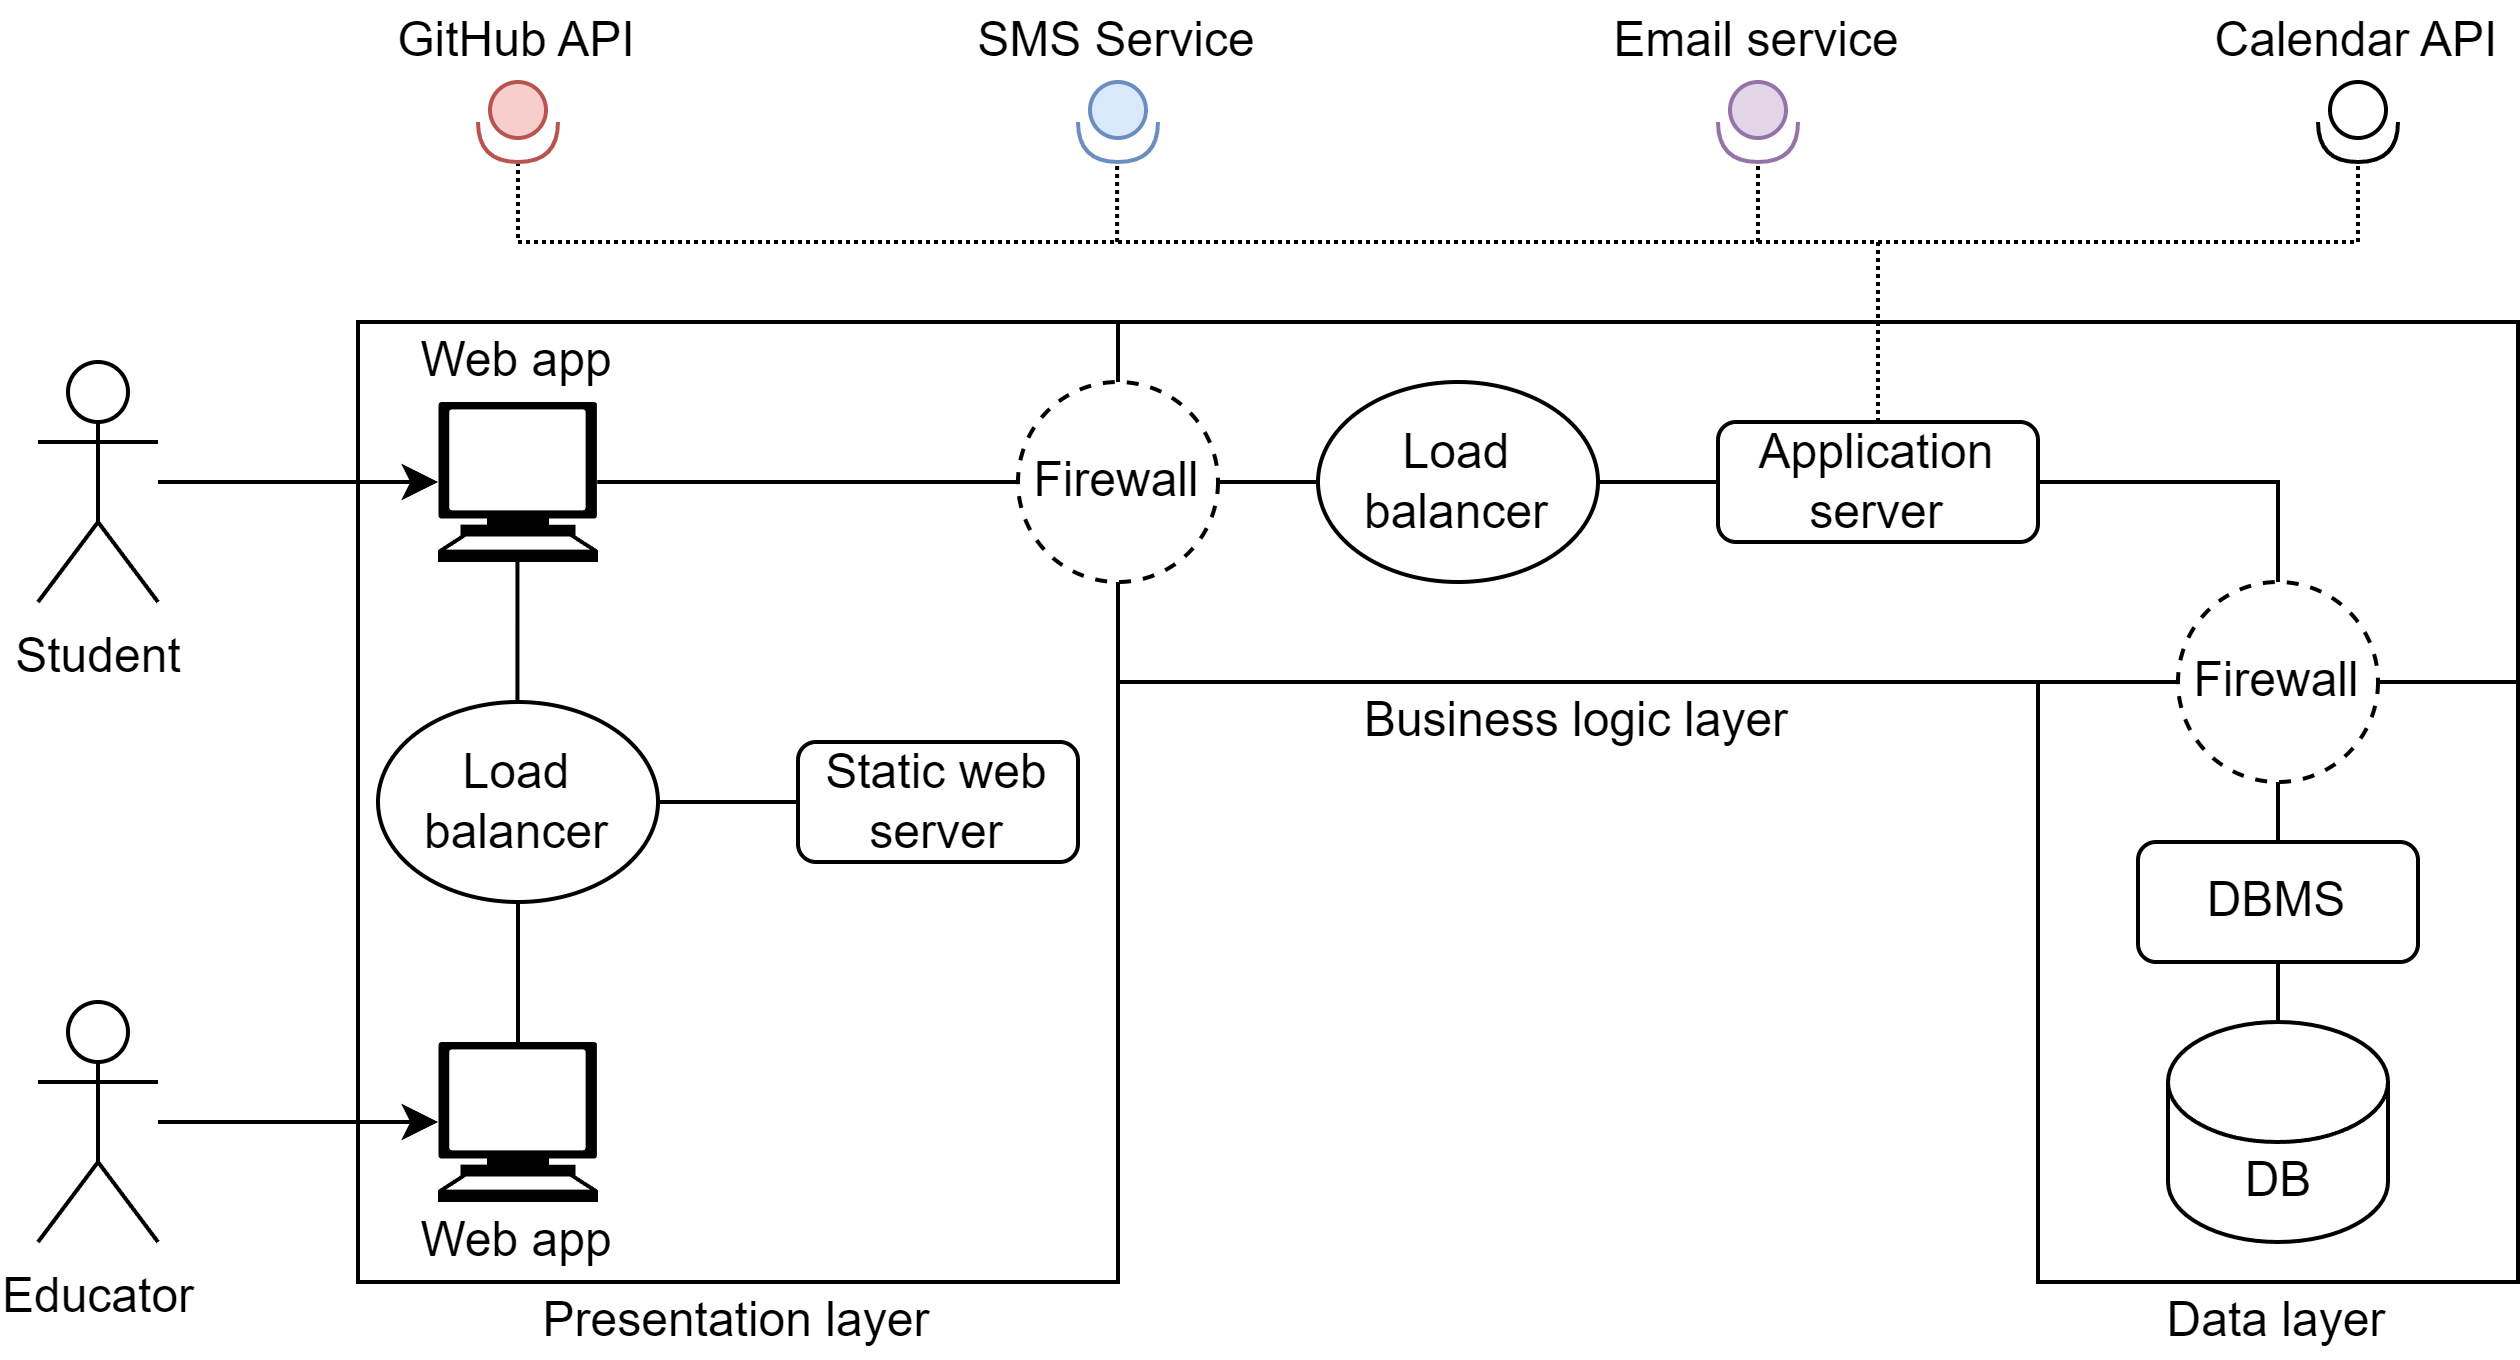
\includegraphics[width=0.9\linewidth]{images/high_level_architecture.png}
    \end{figure}
    The service will be accessed through a web interface, utilizing a single page application (SPA) that proves advantageous for this application type, enabling extensive interaction without frequent page reloads, thereby ensuring a faster and smoother user experience. 
    The system's architecture is structured three into distinct layers, with application servers interacting with a database management system and utilizing APIs for data retrieval and storage. 
    Adhering to REST standards, the application servers are designed to be stateless, and the system incorporates firewalls to bolster security.
    
    \section{Component view}
    \begin{figure}[H]
        \centering
        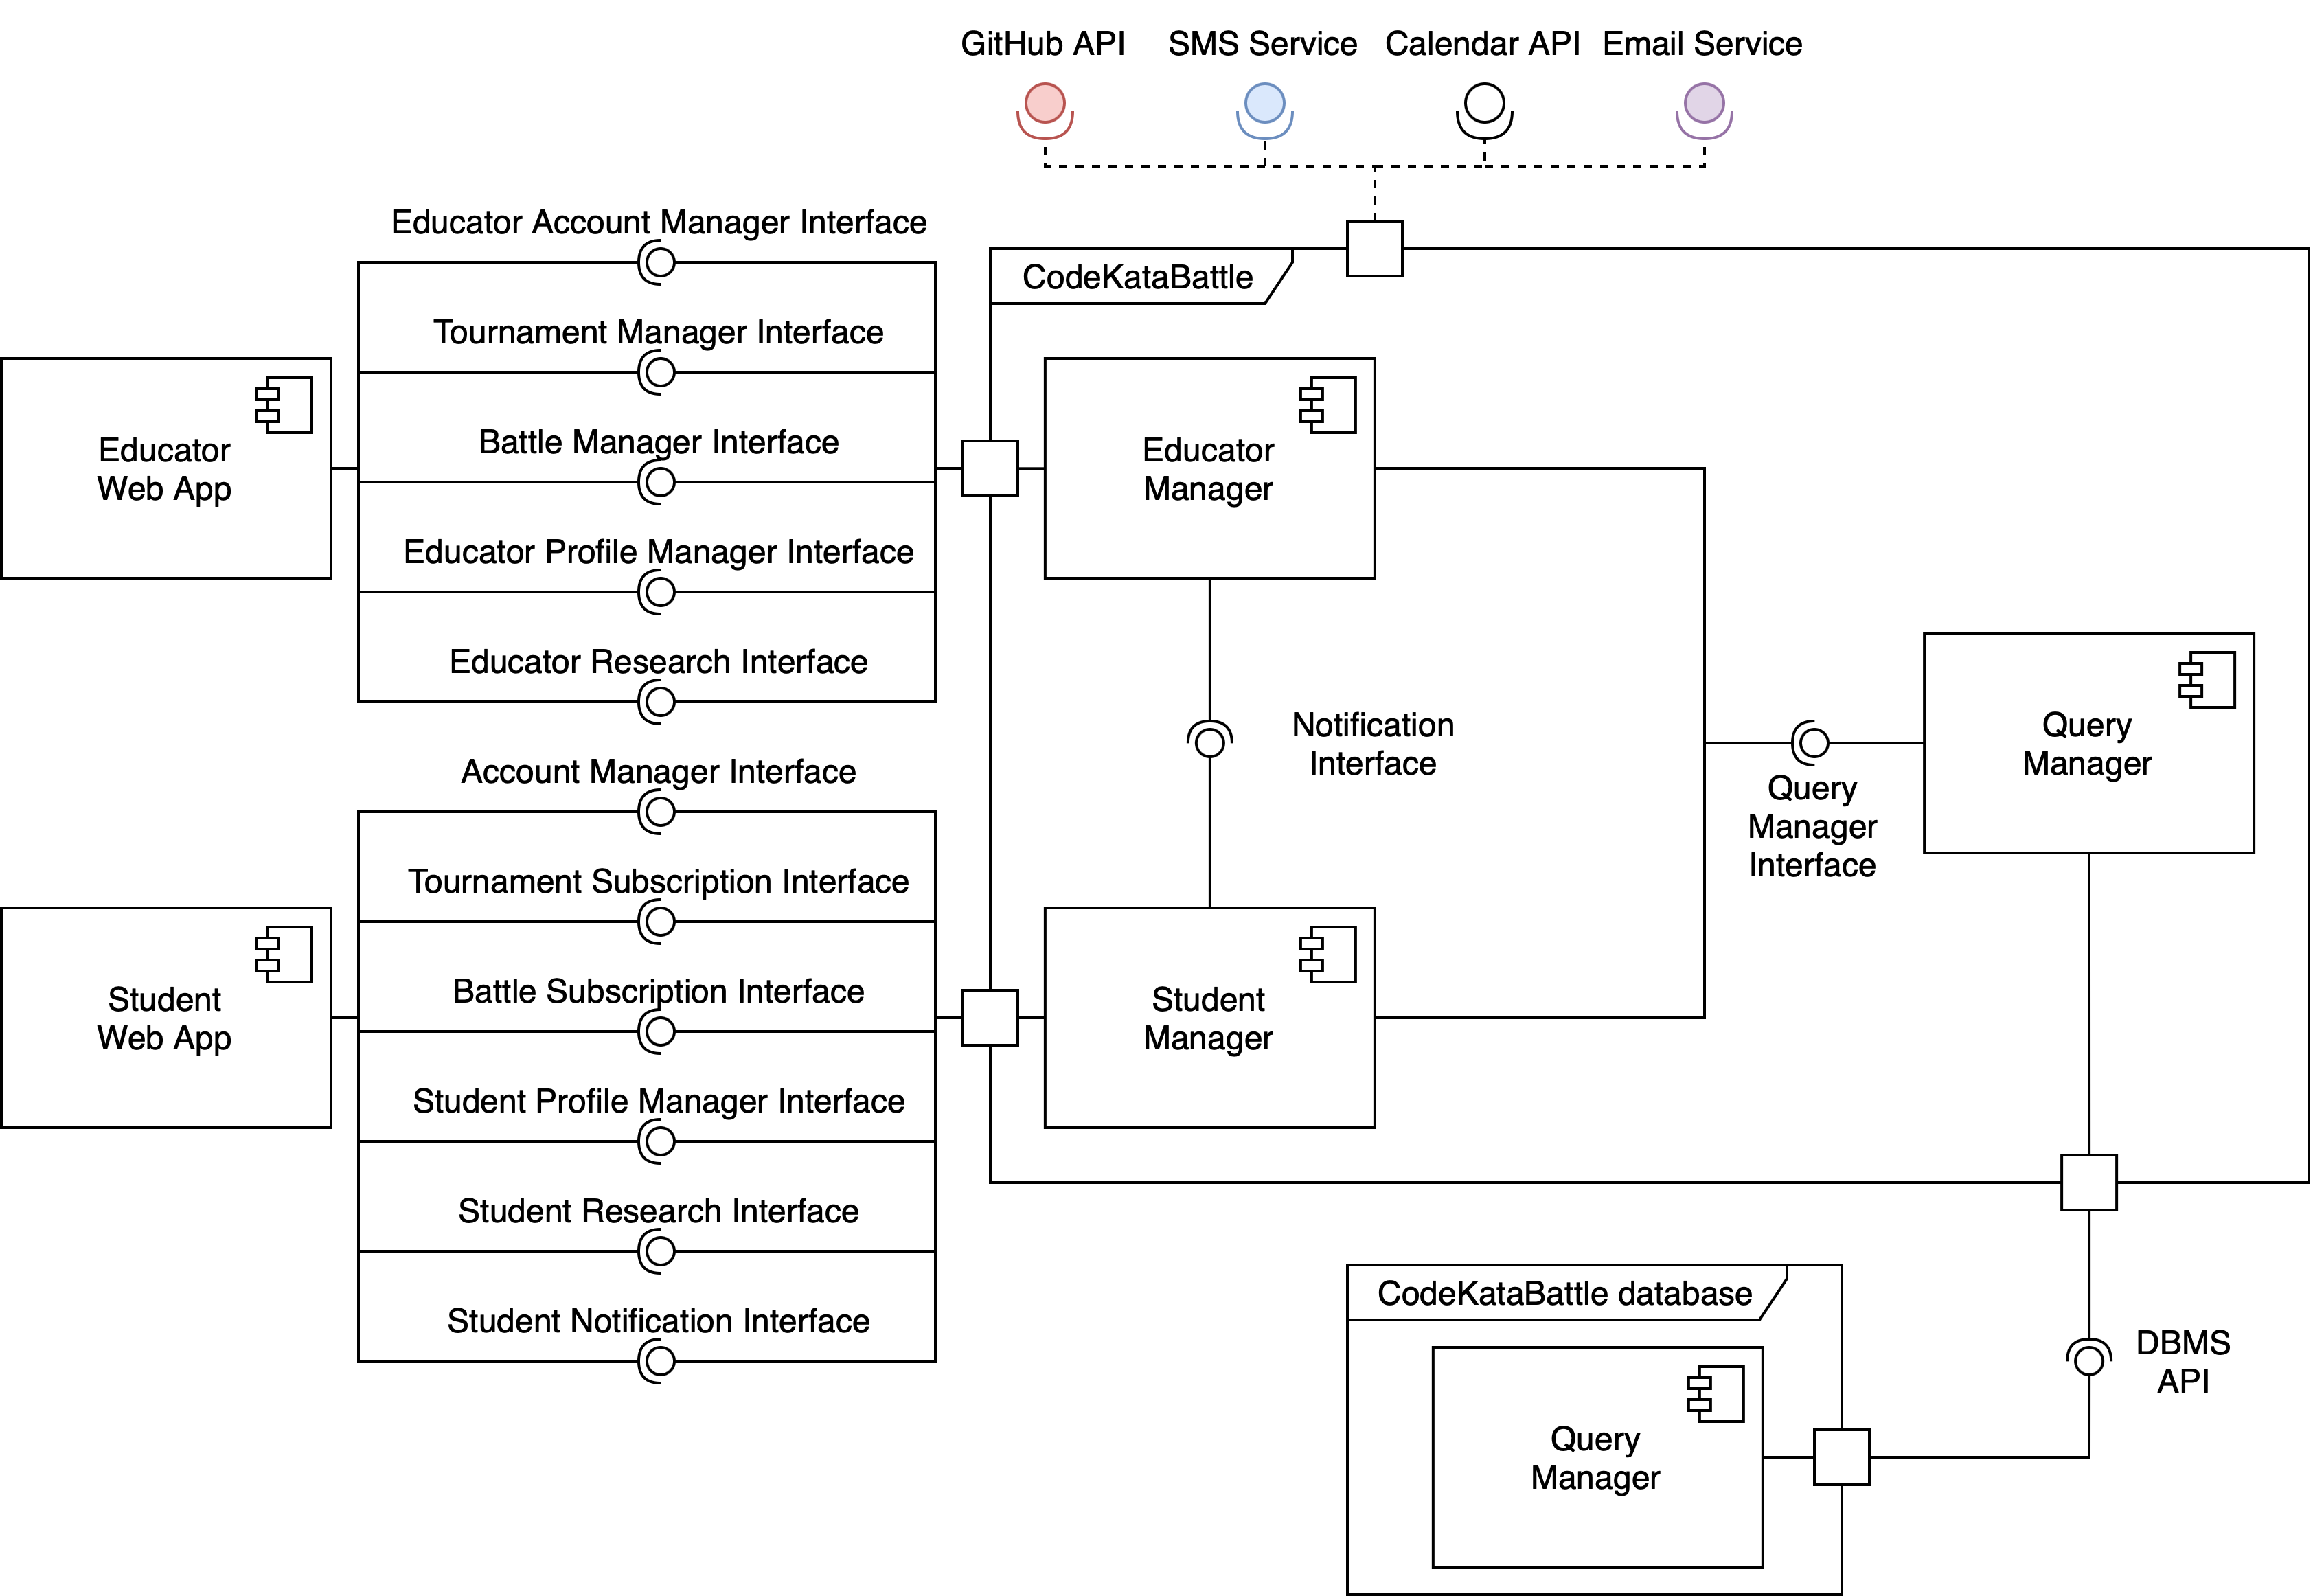
\includegraphics[width=1\linewidth]{images/component_view.png}
        \caption{Component diagram of the CodeKataBattle system}
    \end{figure}
    The component diagram contains all the interfaces used by the educators and the students. 
    These components will be better explained and analyzed in the following pages. 
    Both components have an interface with the database, that deals with the data of all the system. 
    The system has also access to some external API that are inserted at the top of the diagram.  

    \subsection{Query manager}
    This element is tasked with interfacing with a Database Management System (DBMS). 
    It adheres to the Adapter design pattern, enabling seamless interaction between other components and the DBMS without necessitating the manual writing of SQL code.

    \subsection{Educator manager}
    The educator manager component is responsible for interacting with educators.
    It allows the educator to log in, register, manage the profile, search for a tournament, create a tournament, create a battle, check the leaderboards, manage a tournament and give points to the students. 
    \begin{figure}[H]
        \centering
        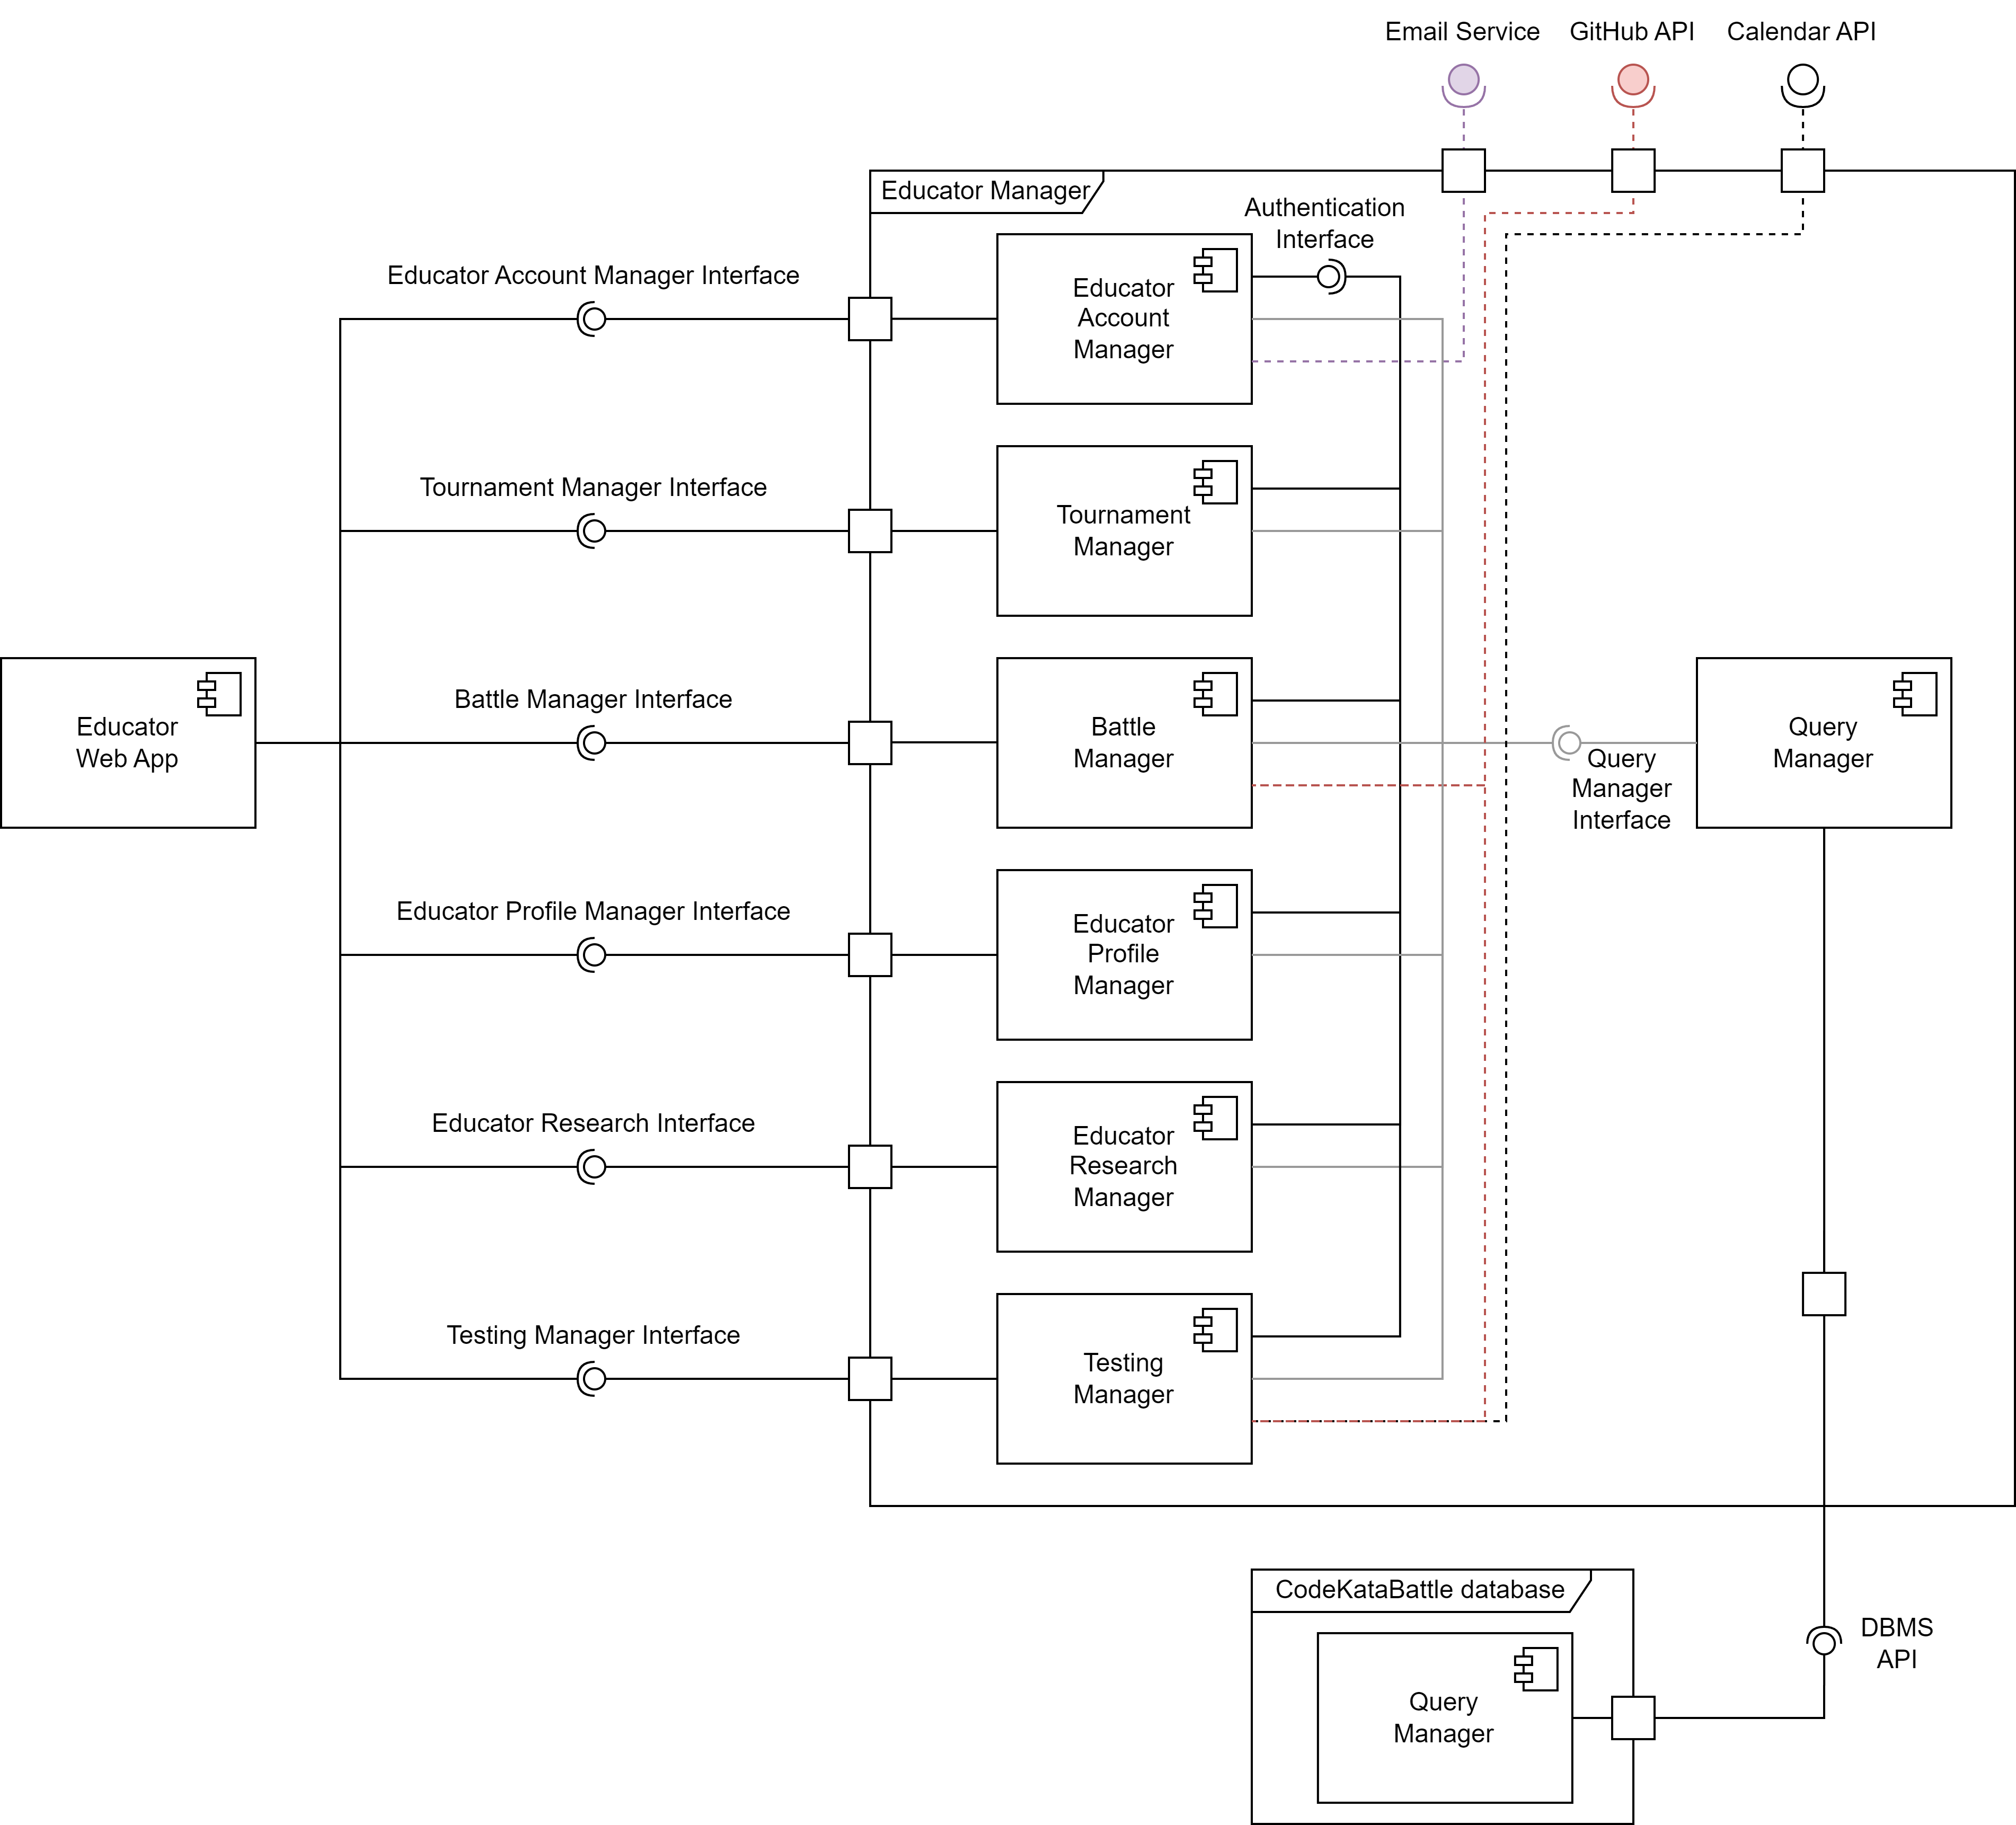
\includegraphics[width=0.8\linewidth]{images/component_view_educator.png}
    \end{figure}
    The educator manager component is expanded in five component as follows: 
    \begin{itemize}
        \item \textit{Educator Account Manager}: this component allows the educators to log in and register to the system.
            It has an authentication interfaces that allows all other components to check if the educator is logged in and is allowed to do certain actions. 
            The account manager is also linked to the database through the query manager interface, that allows it to manage data in the tables dedicated to the educator.
            The only external API used by it is the email service that is utilized to verify the email whenever a new educator tries to register. 
        \item \textit{Tournament Manager}: this component allows the educators to manage a tournament with the following actions: create a tournament, add a collaborator to a tournament, and close a tournament. 
            It has a connection to the authentication manager since it needs to verify the user that is trying to modify the tournament. 
            The tournament manager is also linked to the database through the query manager interface, that allows it to gather and add data to the tables dedicated to the tournament.
            The only external API used by it is the calendar API that is utilized to check the current date and the closure date of the tournament.
        \item \textit{Battle Manager}: this component allows the educators to manage a battle with the following actions: create a battle in a managed tournament, give personal evaluation (that modifies the group point), and close a battle. 
            It has a connection to the authentication manager since it needs to verify the user that is trying to modify the battle. 
            The battle manager is also linked to the database through the query manager interface, that allows it to gather and add data to the tables dedicated to the battle.
            The external APIs used by this component are: GitHub API to create the repository linked to the battle, SMS service to notify the user on the event of the newly created battle, and calendar API to check the main deadlines and notify the educators that manage the battle.
        \item \textit{Educator Profile Manager}: this component allows the educators to check the personal profile with personal information and tournaments information. 
            It has an authentication interface that allows all other components to check if the educator is logged in and is allowed to check the desired profile. 
            The profile manager is also linked to the database through the query manager interface, that allows it to manage data in the tables dedicated to the educator's profile.
        \item \textit{Educator Research Manager}: this component allows the educators to search all the active tournament in the system and to check all the leaderboards and rankings. 
            It has an authentication interface that allows all other components to check if the educator is logged in.
            The research manager is also linked to the database through the query manager interface, that allows it to manage data in the tables dedicated to the tournaments.
        \item \textit{Testing Manager}: this component is used to give the automatic evaluation to a code whenever there is a new push in a repository. 
            This component is also used to pull the code from the repository. 
            The testing manager is also linked to the database through the query manager interface, that allows it to manage data in the tables dedicated to the battles.
    \end{itemize}
    
    \newpage

    \subsection{Student manager}
    The student manager component is responsible for interacting with students.
    It allows the student to log in, register, manage the profile, search for a tournament, join a tournament, join a battle, and check the leaderboards.  
    \begin{figure}[H]
        \centering
        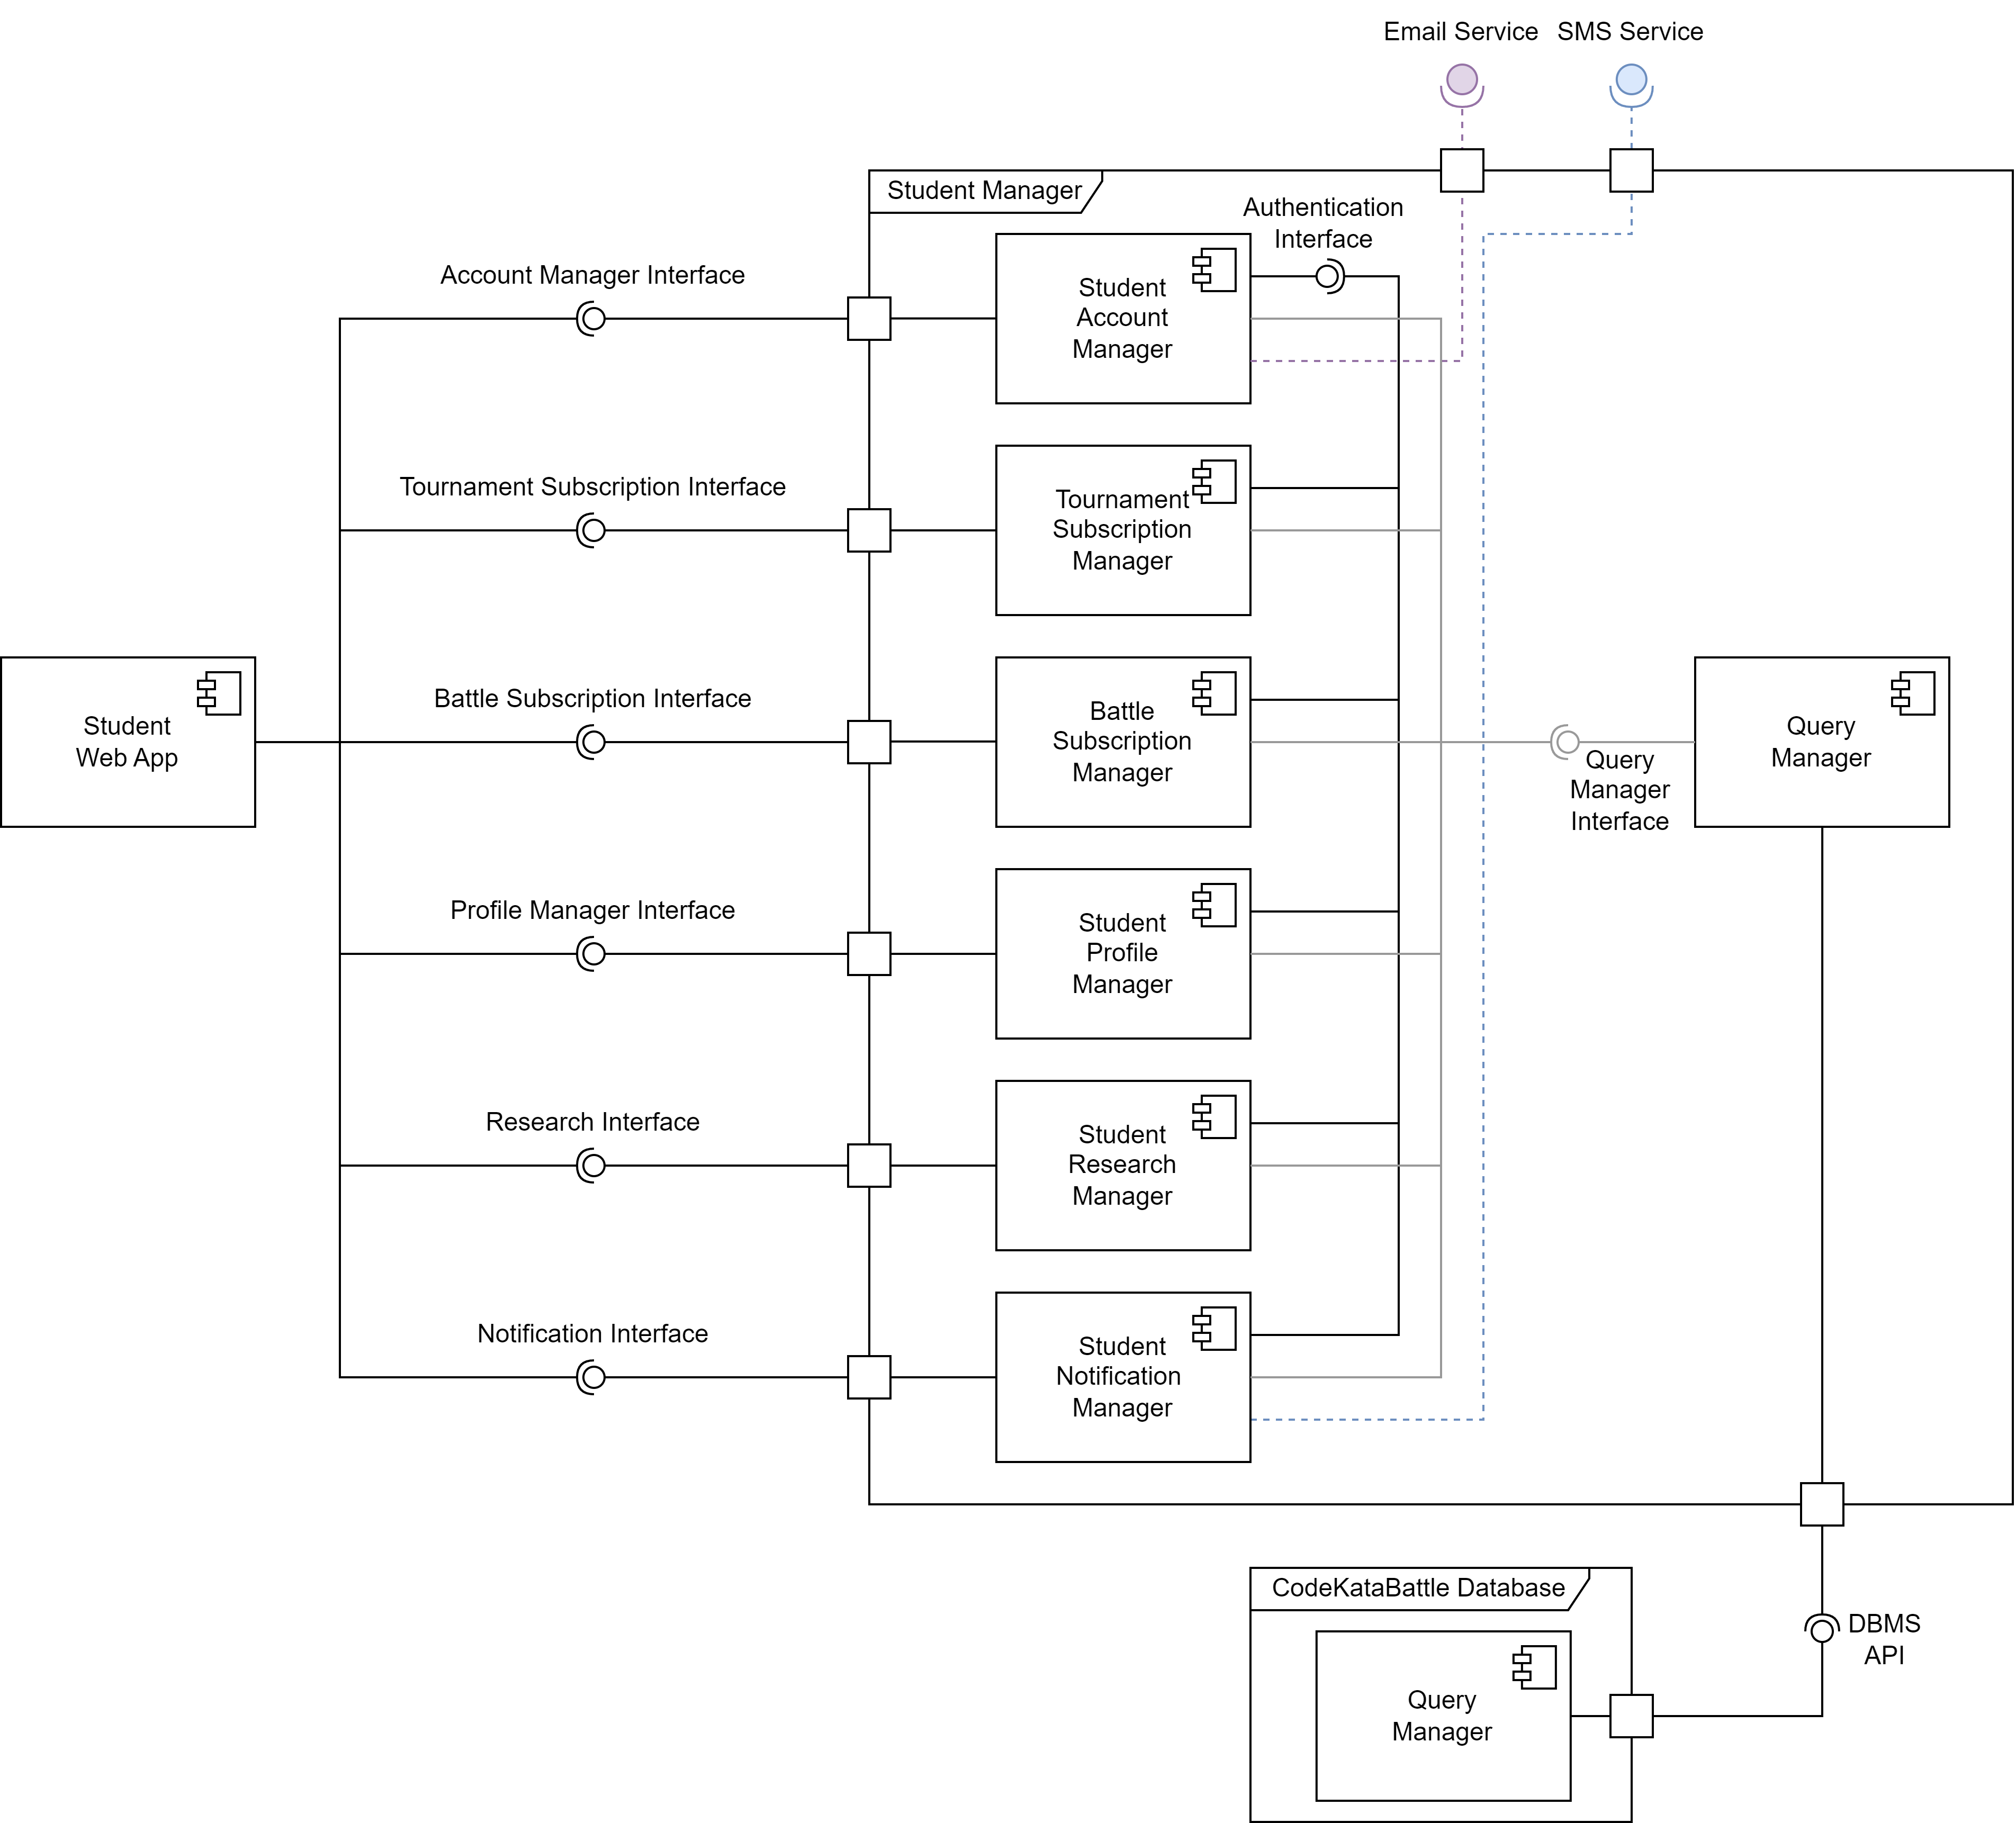
\includegraphics[width=0.8\linewidth]{images/component_view_student.png}
    \end{figure}
    The student manager component is expanded in five component as follows: 
    \begin{itemize}
        \item \textit{Student Account Manager}: this component allows the students to log in and register to the system.
            It has an authentication interfaces that allows all other components to check if the student is logged in and is allowed to do certain actions. 
            The account manager is also linked to the database through the query manager interface, that allows it to manage data in the tables dedicated to the student.
            The only external API used by it is the email service that is utilized to verify the email whenever a new student tries to register. 
        \item \textit{Tournament Subscription Manager}: this component allows the students to enroll in a tournament with the following actions.
            It has a connection to the authentication manager since it needs to verify the user that is trying to enroll in a tournament. 
            The tournament subscription manager is also linked to the database through the query manager interface, that allows to register the student to the tournament. 
            The external APIs used by this component are: SMS service to notify the user on the event of the tournament, and calendar API to check the main deadlines and notify the students that are enrolled in the tournament.
        \item \textit{Battle Subscription Manager}: this component allows the students to enroll in a battle within a tournament where they are already subscribed. 
            It has a connection to the authentication manager since it needs to verify the user that is trying to enroll in the battle. 
            The battle subscription manager is also linked to the database through the query manager interface, that allows it to gather and add data to the tables dedicated to the battle.
            The external APIs used by this component are the SMS service to notify the user on the event of the newly created battle, and the calendar API to check the main deadlines and notify the students that are enrolled in the battle.
        \item \textit{Student Profile Manager}: this component allows the students to check the personal profile with personal information and enrolled tournaments information. 
            It has an authentication interfaces that allows all other components to check if the student is logged in and is allowed to check the desired profile. 
            The profile manager is also linked to the database through the query manager interface, that allows it to manage data in the tables dedicated to the student's profile.
        \item \textit{Student Research Manager}: this component allows the students to search all the active tournament in the system and to check all the leaderboards and rankings. 
            It has an authentication interfaces that allows all other components to check if the student is logged in.
            The research manager is also linked to the database through the query manager interface, that allows it to manage data in the tables dedicated to the tournaments.
        \item \textit{Student Notification Manager}: this component allows the user to be notified when a tournament is created or modified and when new battles are added. 
            It has an interface with the Educator Manager since it needs to be used when some Educators create new battles or tournaments.
    \end{itemize}

    \newpage
    \subsection{Database schema}
    In this section there is the E-R schema used for the database of the system. 
    \begin{figure}[H]
        \centering
        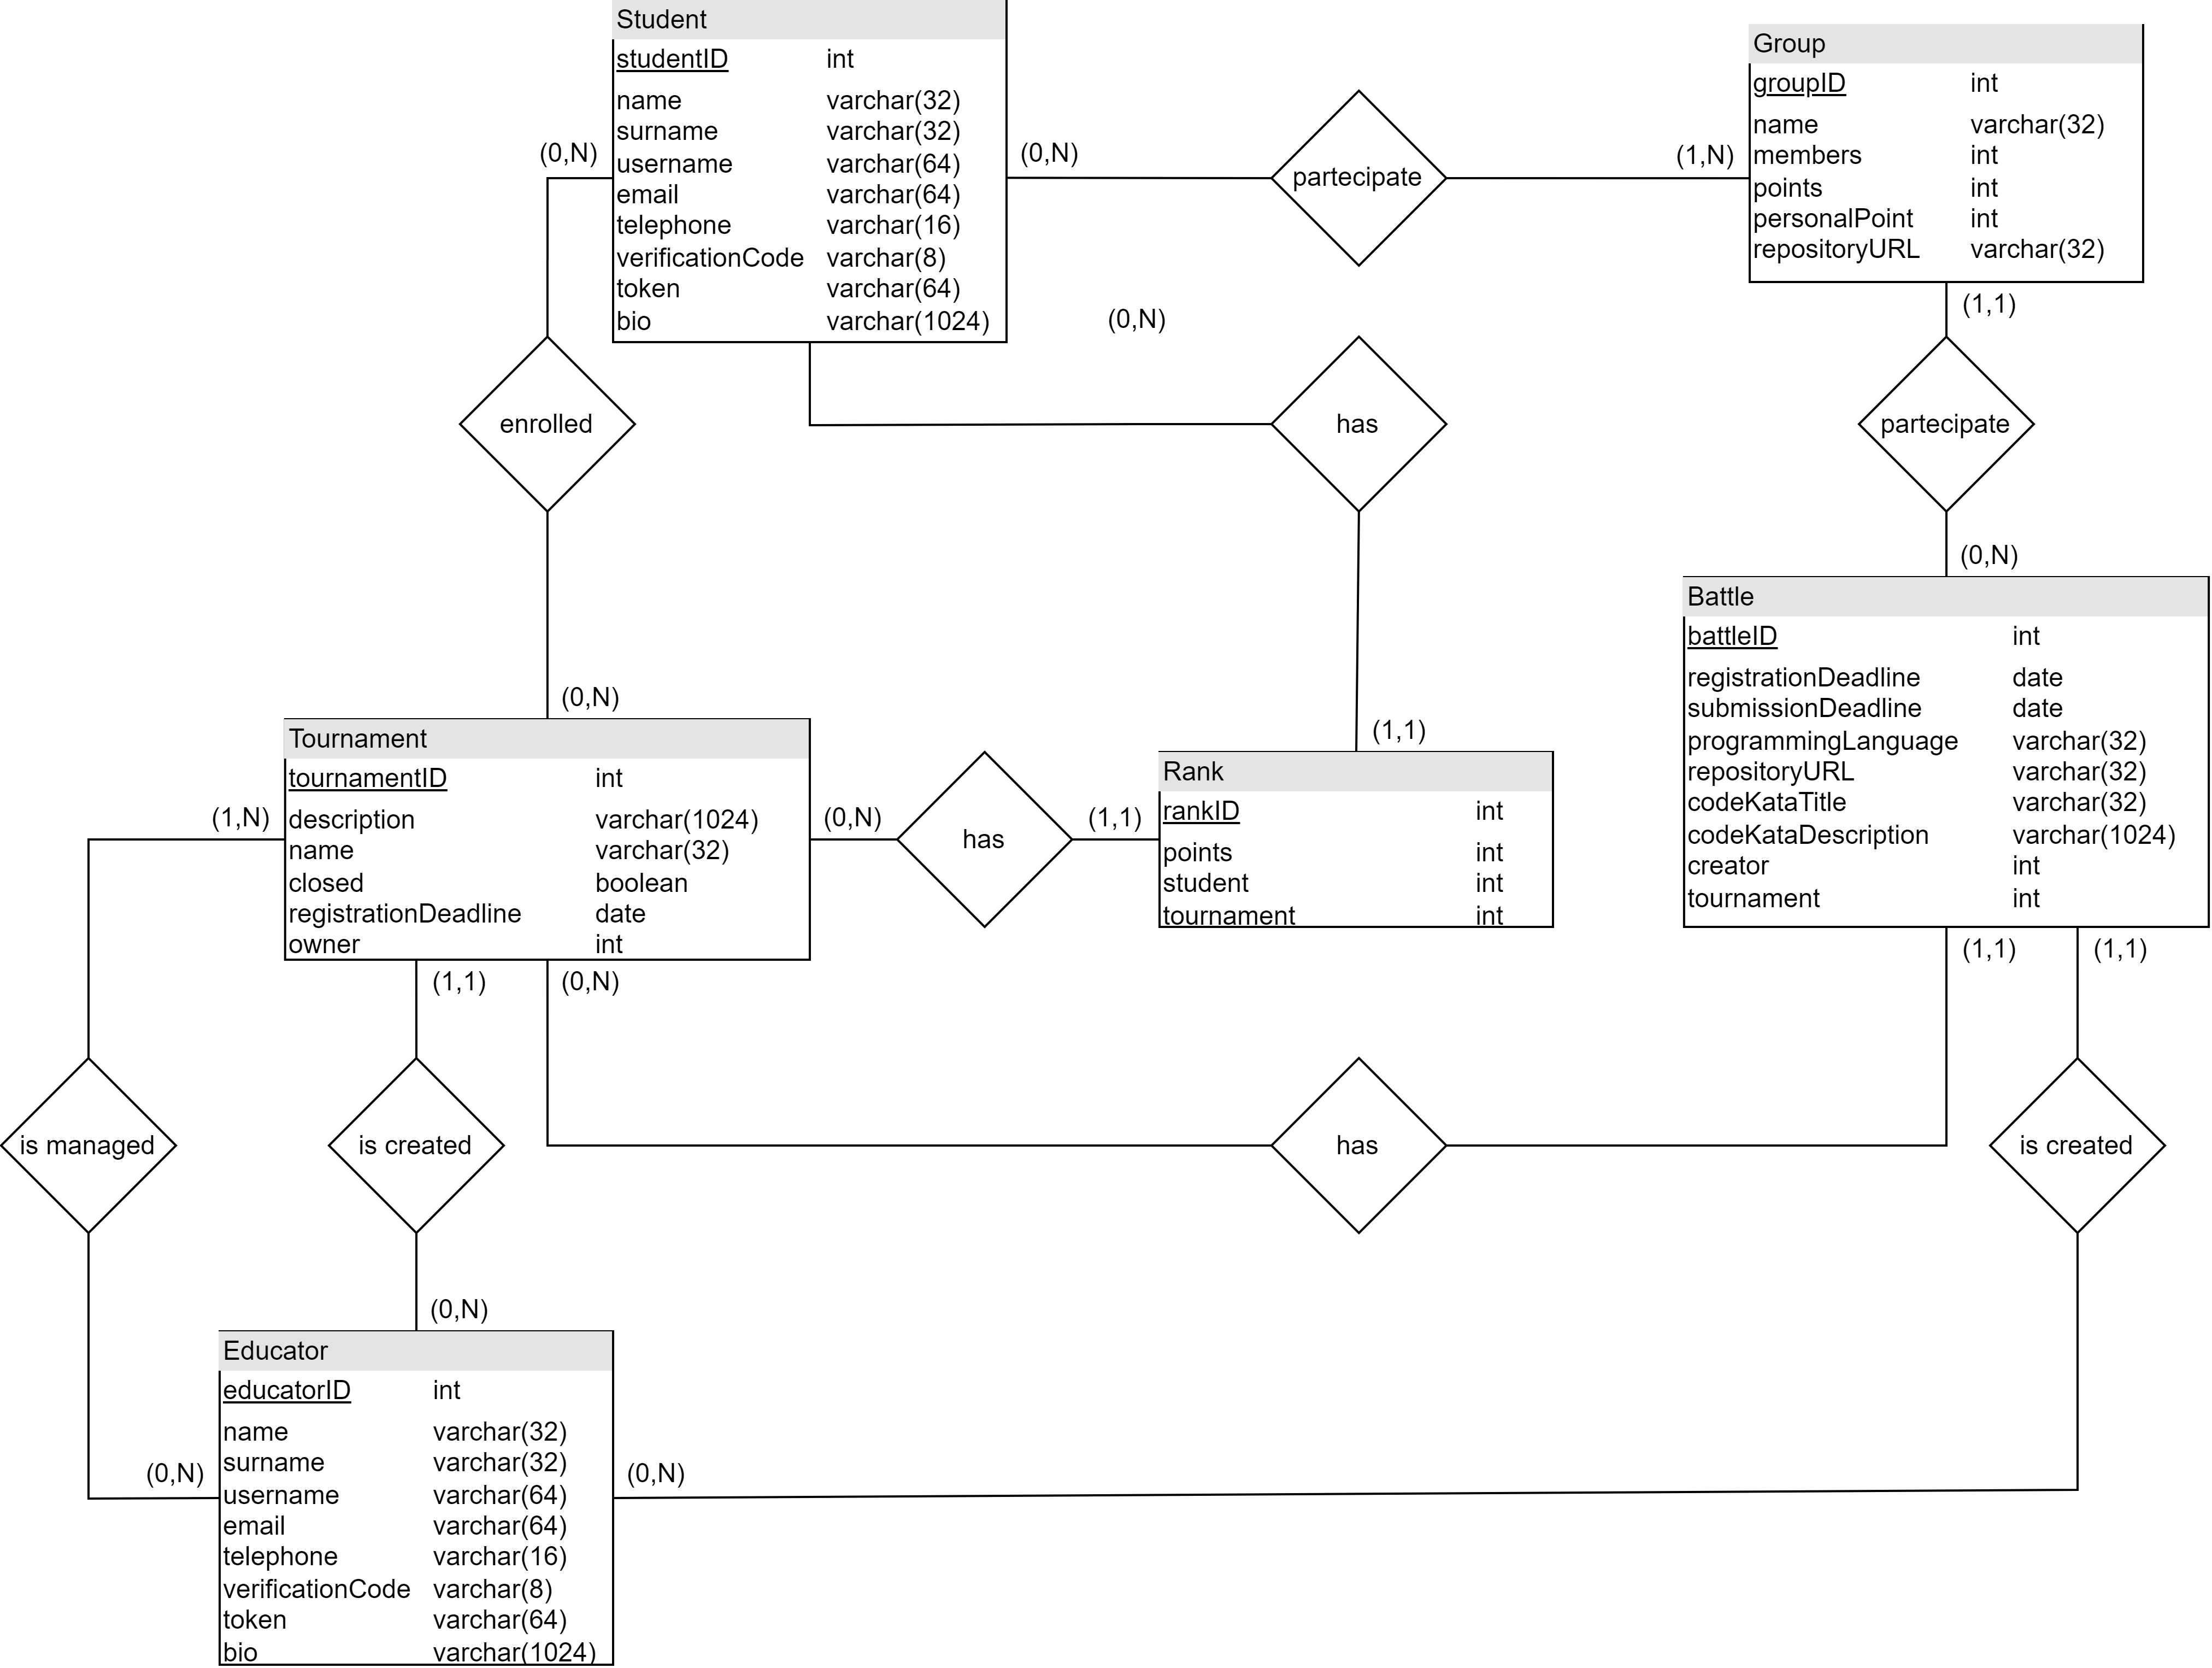
\includegraphics[width=0.9\linewidth]{images/db.png}
    \end{figure}
    Students and educators are stored in different tables to have better performance when searching the user in the database.
    The attributes of both tables are the same, and comprises: name, surname, username, email, and telephone. 
    Each student and educator has a unique numerical ID (it is possible to use also the username since we have the uniqueness constraint on it). 

    Group is a table that contains all the groups linked to all the existing battles. 
    It has the following attributes: name, members (the number of members in the considered group), points (of the group in a battle), and repositoryURL (a string with the URL of the group repository for a battle).
    The ID is unique over all possible groups in all possible battles.
    
    Battle represents a single battle with the description of the problem associated with it. 
    The attributes are: registrationDeadline, submissionDeadline, programmingLanguage, repositoryURL (of the general repository to be forked), codeKataTitle, CodeKataDescription, creator (that is the ID of the educator that created the battle), and tournament (that is the ID of the tournament where the battle were created). 
    The ID is unique in the whole system. 

    Tournament represents the list of tournament that have ended (closed set to one) or are running (closed set to zero). 
    Other attributes are: description, name, registrationDeadline, and owner (that is the ID of the educator that created the tournament initially). 
    Also in this case we have a unique ID as key. 

    Rank contains the point associated to a student (ID of the student) for a certain tournament where he is enrolled (tournament is the ID of the linked tournament). 
    Each rank has a single ID. 


    \section{Deployment view}
    Our setup comprises two essential components: a static web server serving as the entry point for clients to access the Single Page Application (SPA), and an application server providing the requisite APIs for the SPA's functionality. 
    To optimize performance and leverage distinct advantages, we've adopted distinct solutions for each part.
    The static web server is deployed on a Content Delivery Network (CDN) to ensure rapid response times. 
    This is achieved through the utilization of edge location caches and reverse proxies. 
    On the other hand, the application server, encompassing both a business logic layer and a data tier, is hosted on a cloud provider. 
    This choice offers several benefits over conventional in-house hosting:
    \begin{itemize}
        \item \textit{Scalability and flexibility}: the cloud infrastructure allows us to dynamically adjust resources such as virtual machines, performance cores, or memory based on demand. Incorporating load balancing services enables the application server to seamlessly adapt to fluctuations in traffic or workload.
        \item \textit{Security}: leveraging services like live monitoring and firewalls enhances the security posture of the application server, safeguarding it against data breaches, cyberattacks, and other security threats.
        \item \textit{Cost-efficiency}: the cloud provider's pay-as-you-go model ensures cost optimization by billing only for the actual resources consumed. This approach proves economical and contributes to lowering overall operational expenses.
    \end{itemize}
    These features collectively position a cloud provider as an optimal choice for hosting large, high-traffic applications. 
    It is imperative that the chosen cloud provider offers comprehensive support for scalability, security, and cost-efficiency to align with our specific requirements.
    \begin{figure}[H]
        \centering
        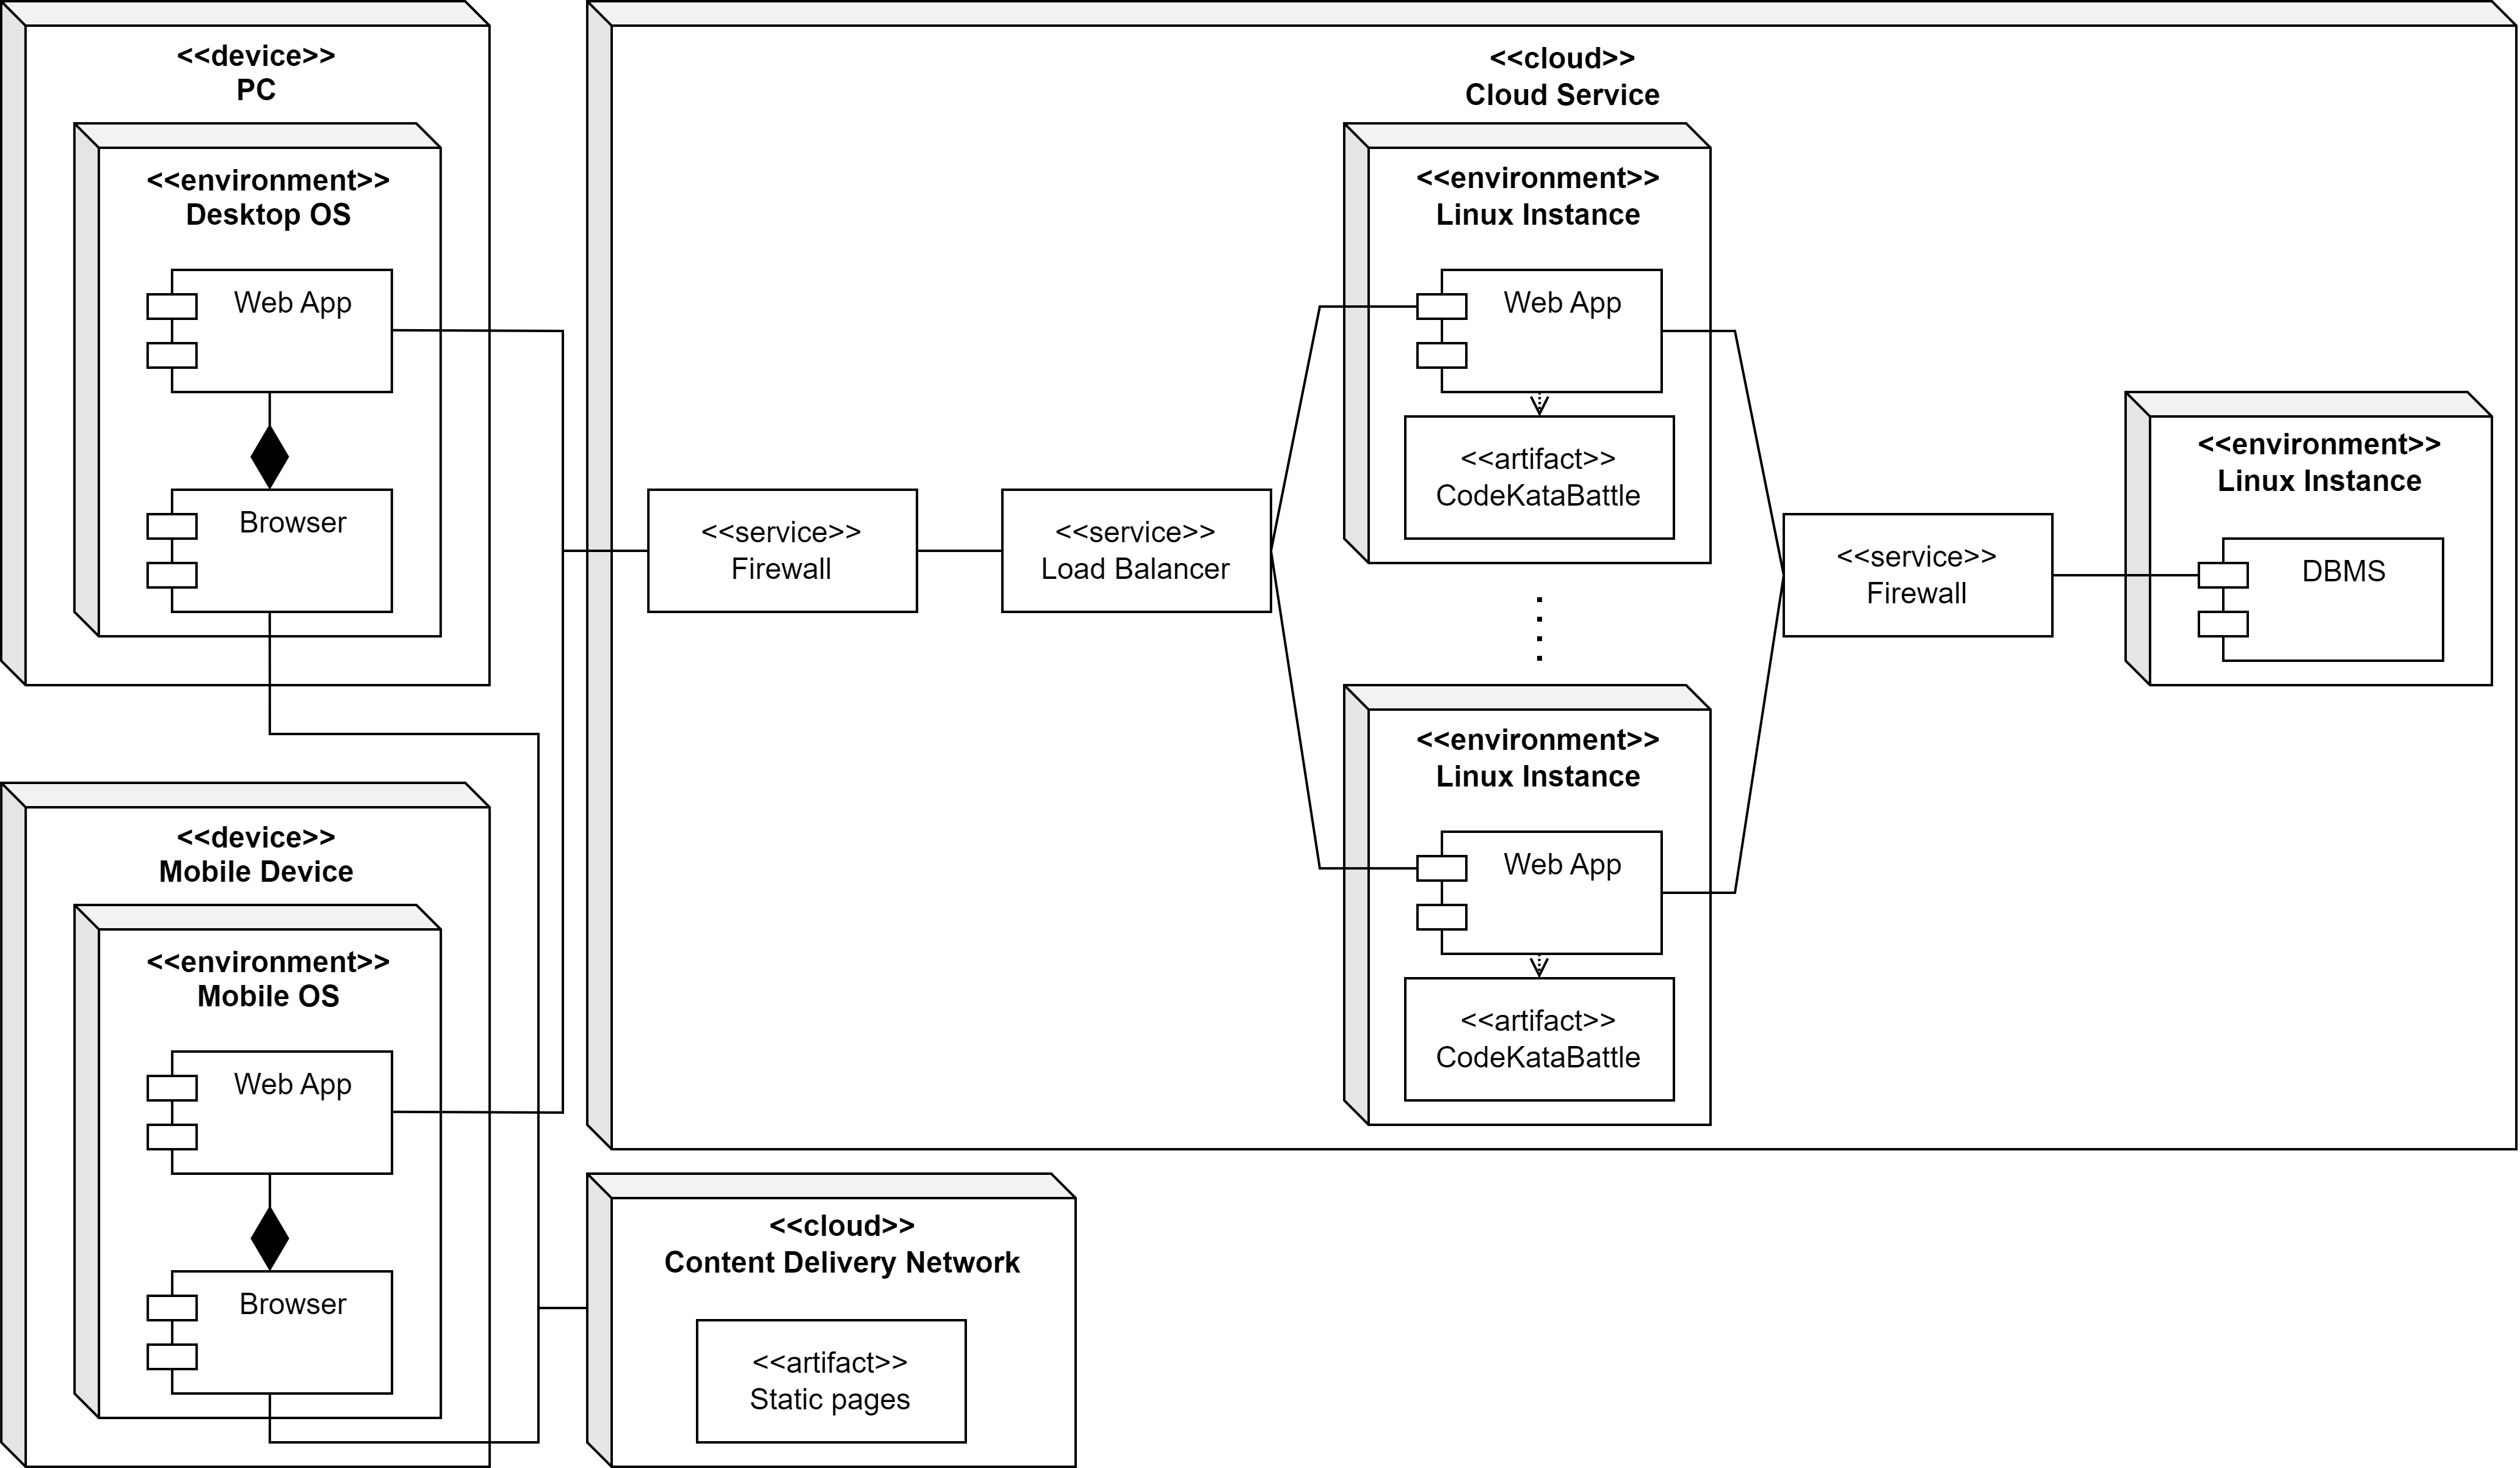
\includegraphics[width=0.9\linewidth]{images/deployment_view.png}
        \caption{Deployment views}
    \end{figure}
    The devices called PC and Mobile are any device with a modern browser capable of running JavaScript. 
    
    The static pages are handled by the Content Delivery Network to avoid affecting the performance of the main application. 
    This part handles the welcome page and login/register pages. 
    These pages are static in the sense that they have no need to have code that runs on server side. 

    Finally, the cloud service will host all the business and data logic. 
    This service contains the following elements: 
    \begin{itemize}
        \item \textit{Firewall services}: employed to filter incoming connections to both the business and data layers of a system, firewall services utilize a predetermined set of rules selected based on specific criteria. 
            This component serves as a crucial defense mechanism against malicious attacks, offering generic filtering capabilities.
        \item \textit{Load balancer}: tasked with distributing incoming traffic among multiple instances of an application, the load balancer serves to optimize resource utilization, enhance performance, and ensure high availability. 
            Its role is critical in preventing application overload or downtime, and it contributes to a stable and reliable user experience by redirecting traffic to the least busy application instance.
        \item \textit{Multiple application instances}: operating in parallel and independently, multiple copies of the application can be dynamically created or deleted to meet demand. 
            This approach enables the application to efficiently handle a high volume of requests without encountering performance issues. 
            Additionally, it provides fault tolerance by redirecting traffic to alternative instances in case one becomes unavailable.
        \item \textit{Data instance}: this component involves a data-optimized virtual machine housing the Database Management System (DBMS) and the associated database. 
            It plays a pivotal role in managing and organizing data efficiently within the system.
    \end{itemize}

    \section{Runtime view}
    \subsection{Student's runtime view}
    In this section we list all possible actions for the student along with the runtime view associated with each one. 
    
    \paragraph*{Student signup}
    In this case the actor is an unregistered student that is trying to sign up in the system.
    After accessing the corresponding page the student submits all the required information to the student account manager component that checks the data. 
    If the user is not already register it creates a new student after the email verification. 
    \begin{figure}[H]
        \centering
        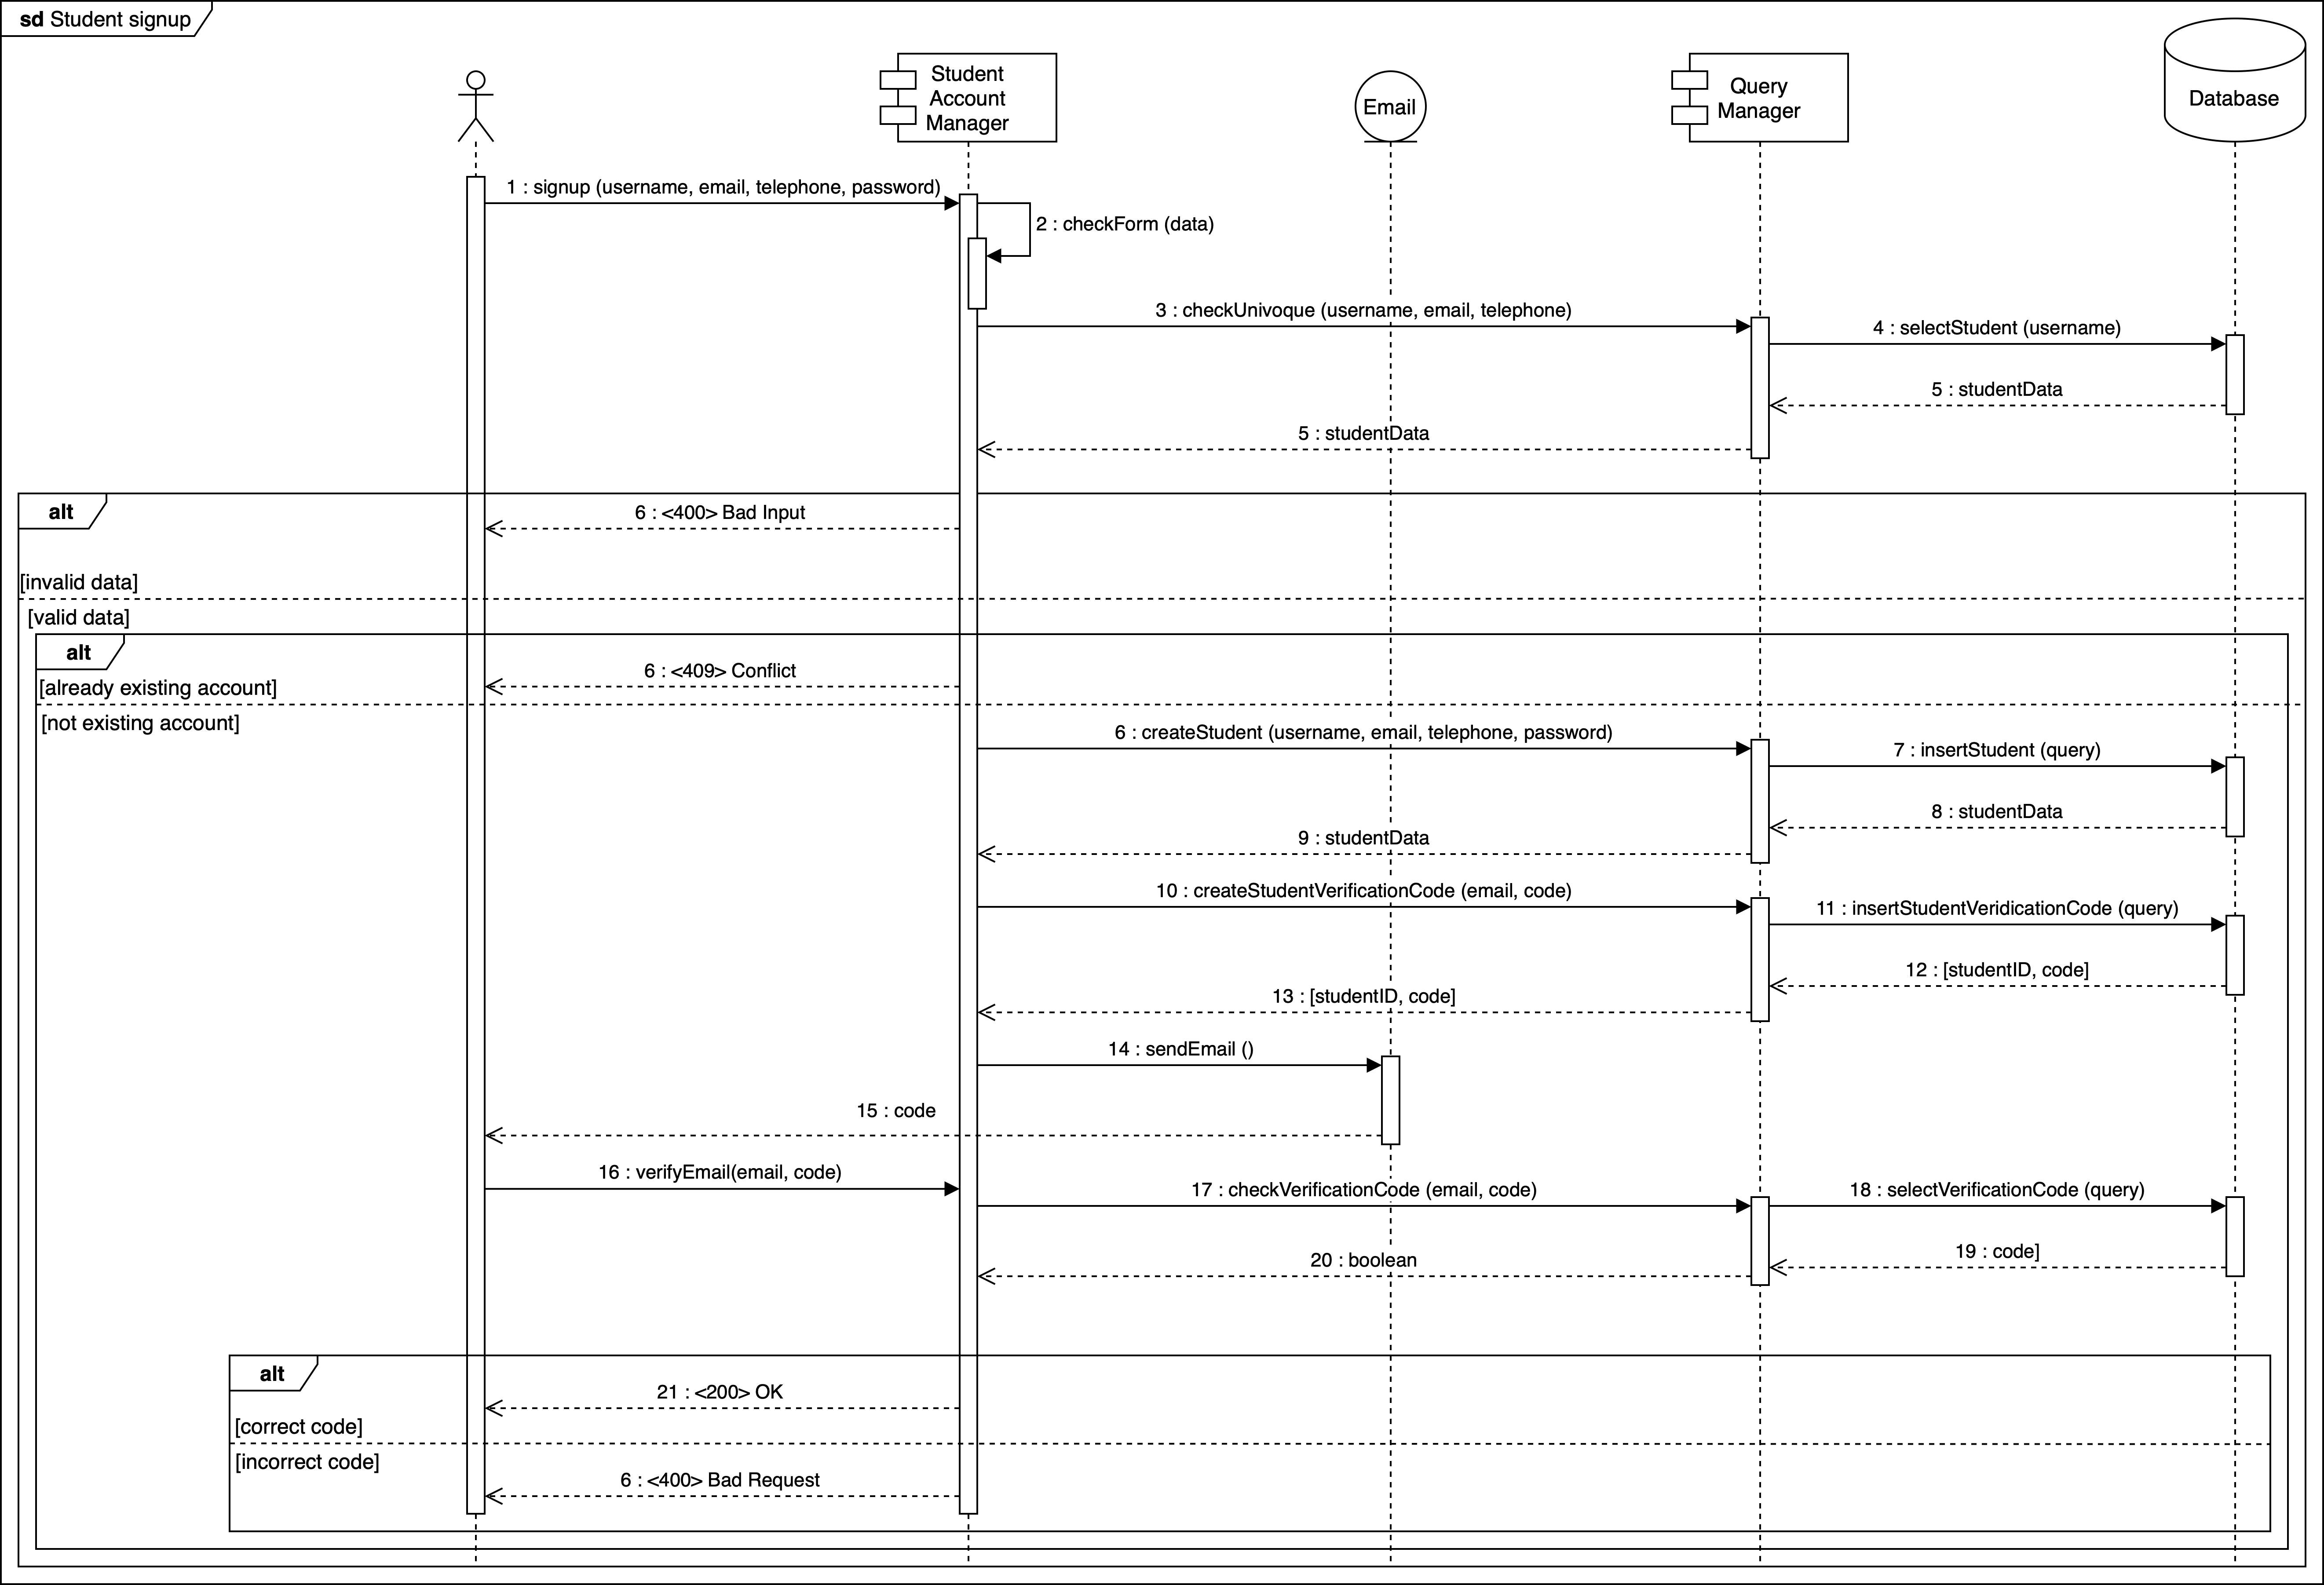
\includegraphics[width=1.0\linewidth]{images/ssrv.png}
    \end{figure}

    \paragraph*{Student log in}
    In this case the actor is a registered student that wants to log in into the system. 
    After accessing the corresponding page the student submits all the required information to the student account manager component that checks the data. 
    If the inserted data are correct the student can access all his possible actions. 
    \begin{figure}[H]
        \centering
        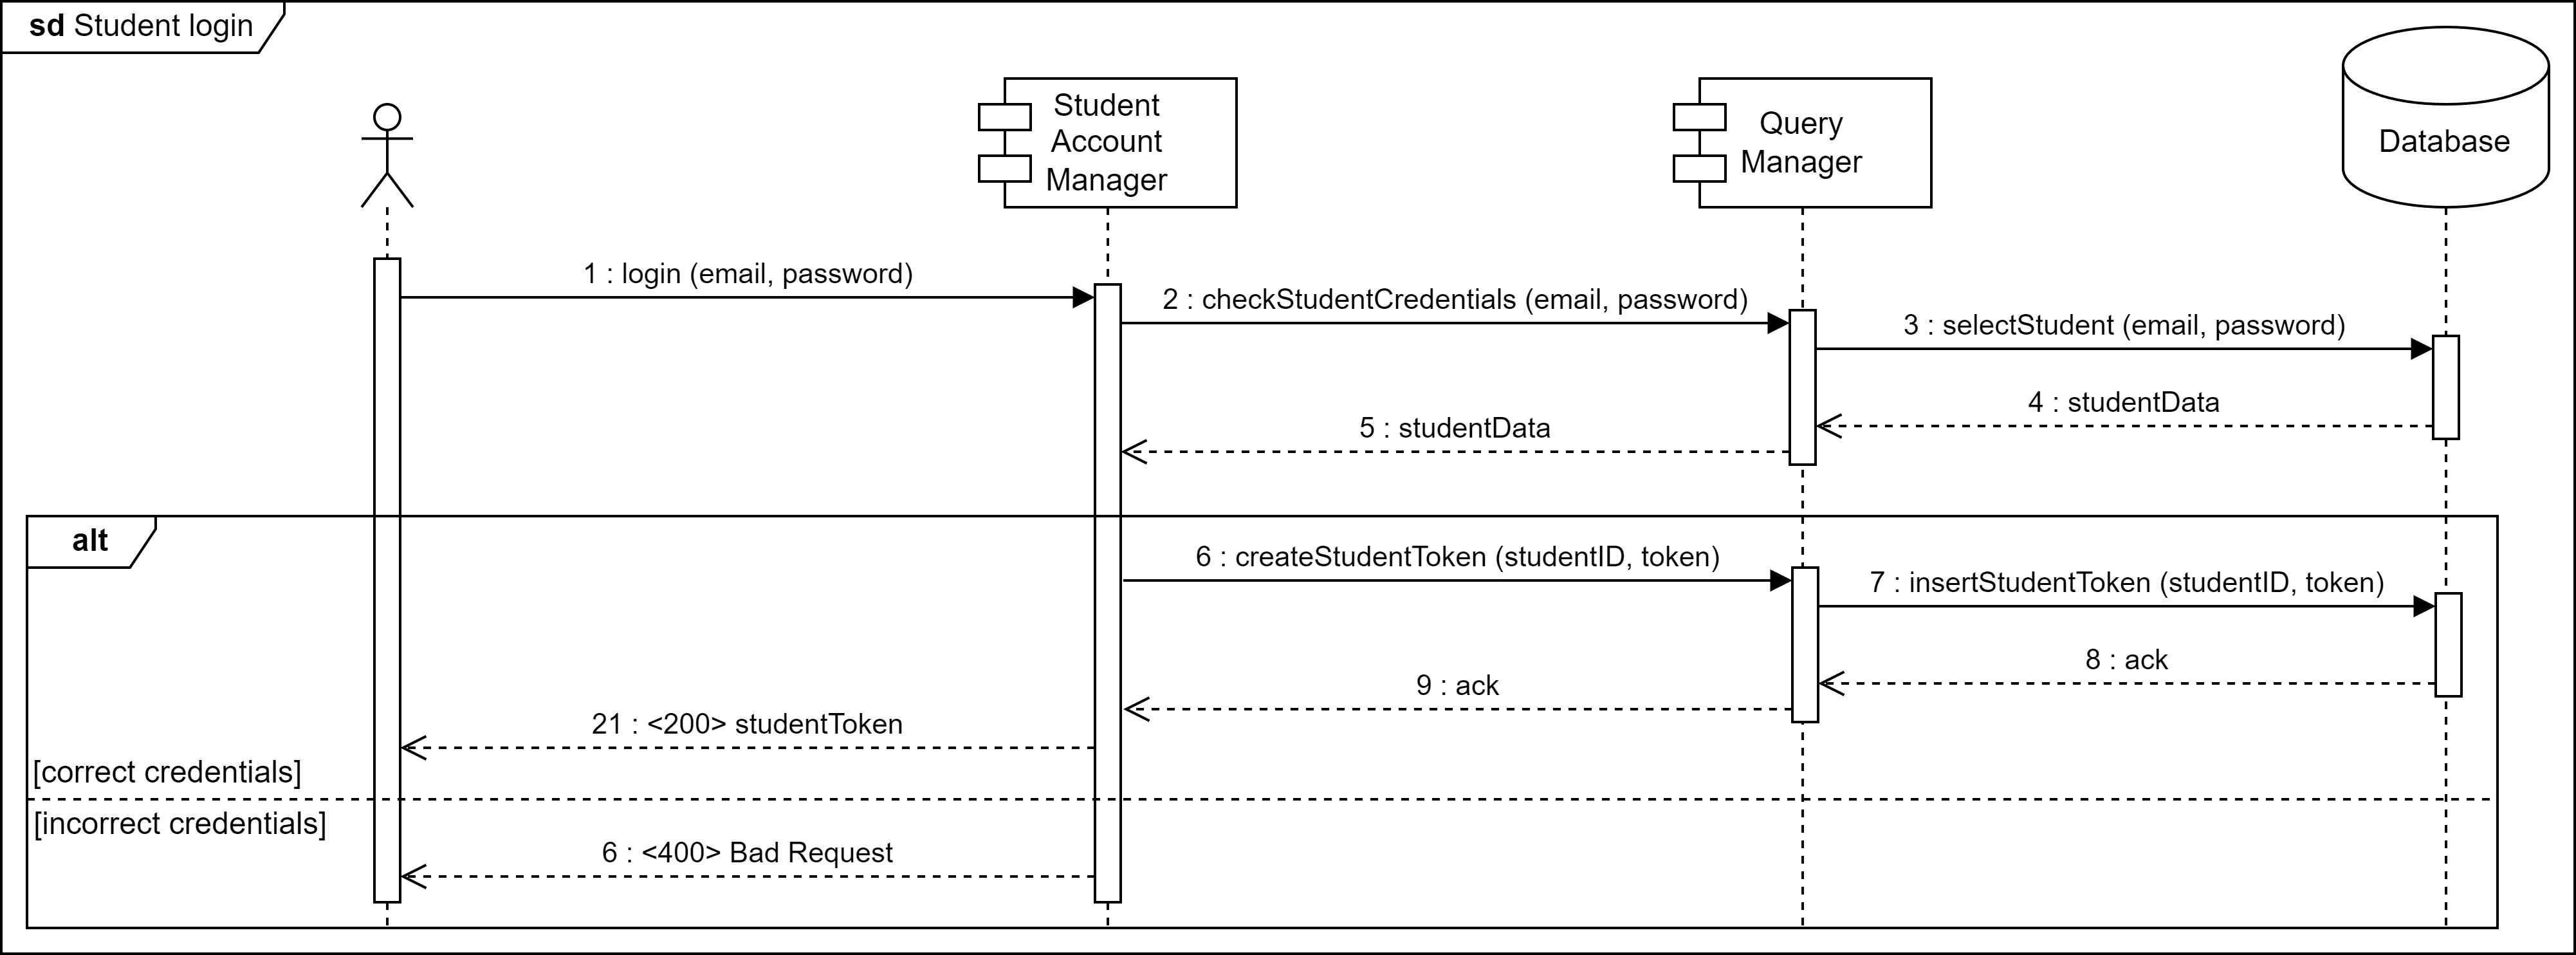
\includegraphics[width=1.0\linewidth]{images/slrv.png}
    \end{figure}

    \paragraph*{Student profile}
    In this case the actor is a registered student that wants to check his own profile. 
    The student profile manager retrieves all the data linked to the student and returns the complete page to the student. 
    \begin{figure}[H]
        \centering
        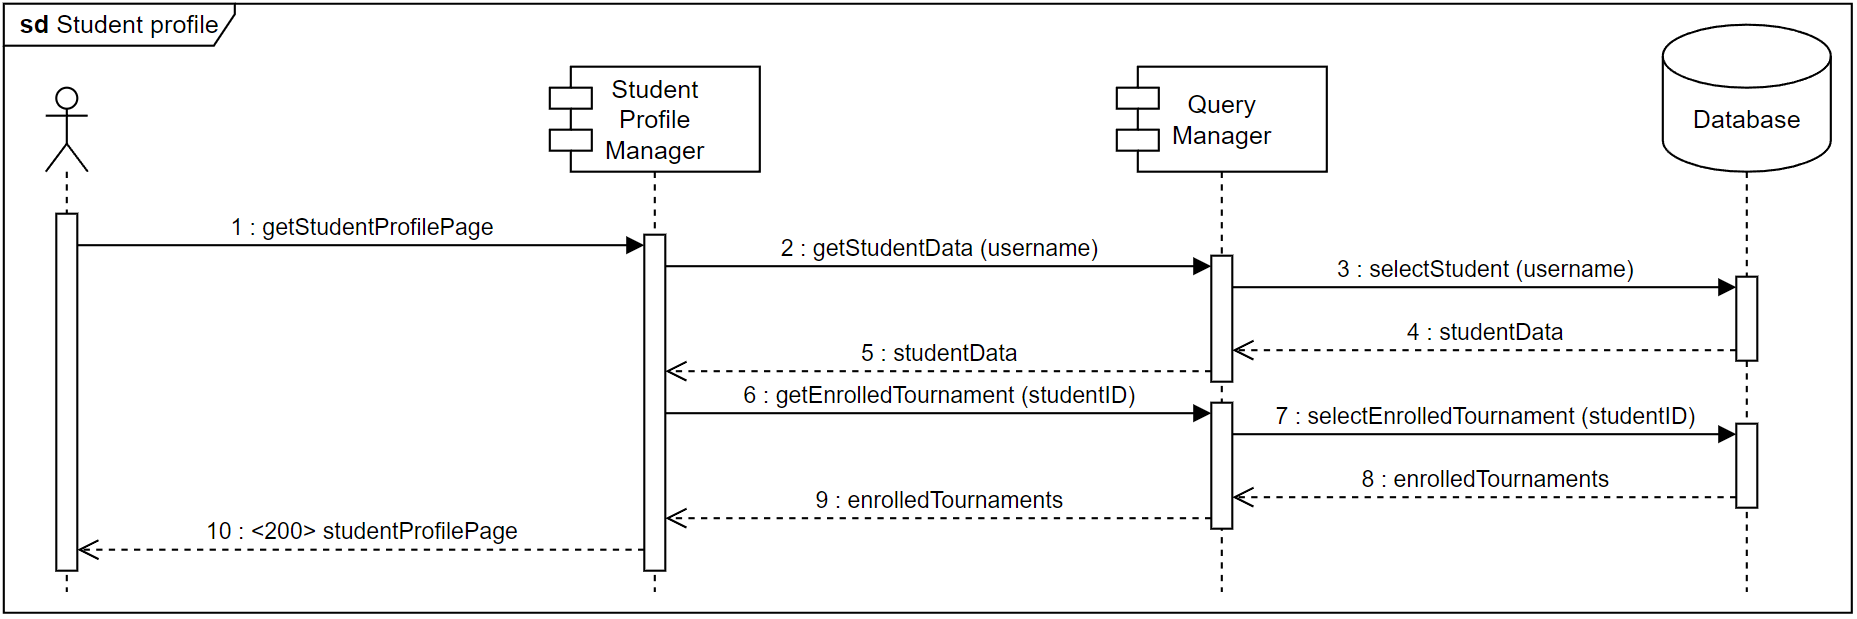
\includegraphics[width=1.0\linewidth]{images/sprv.png}
    \end{figure}

    \paragraph*{Student home page}
    In this case the actor is a registered student that wants to access the home page. 
    The student research manager retrieves all the active tournaments from the database and return the home page with some tournaments. 
    \begin{figure}[H]
        \centering
        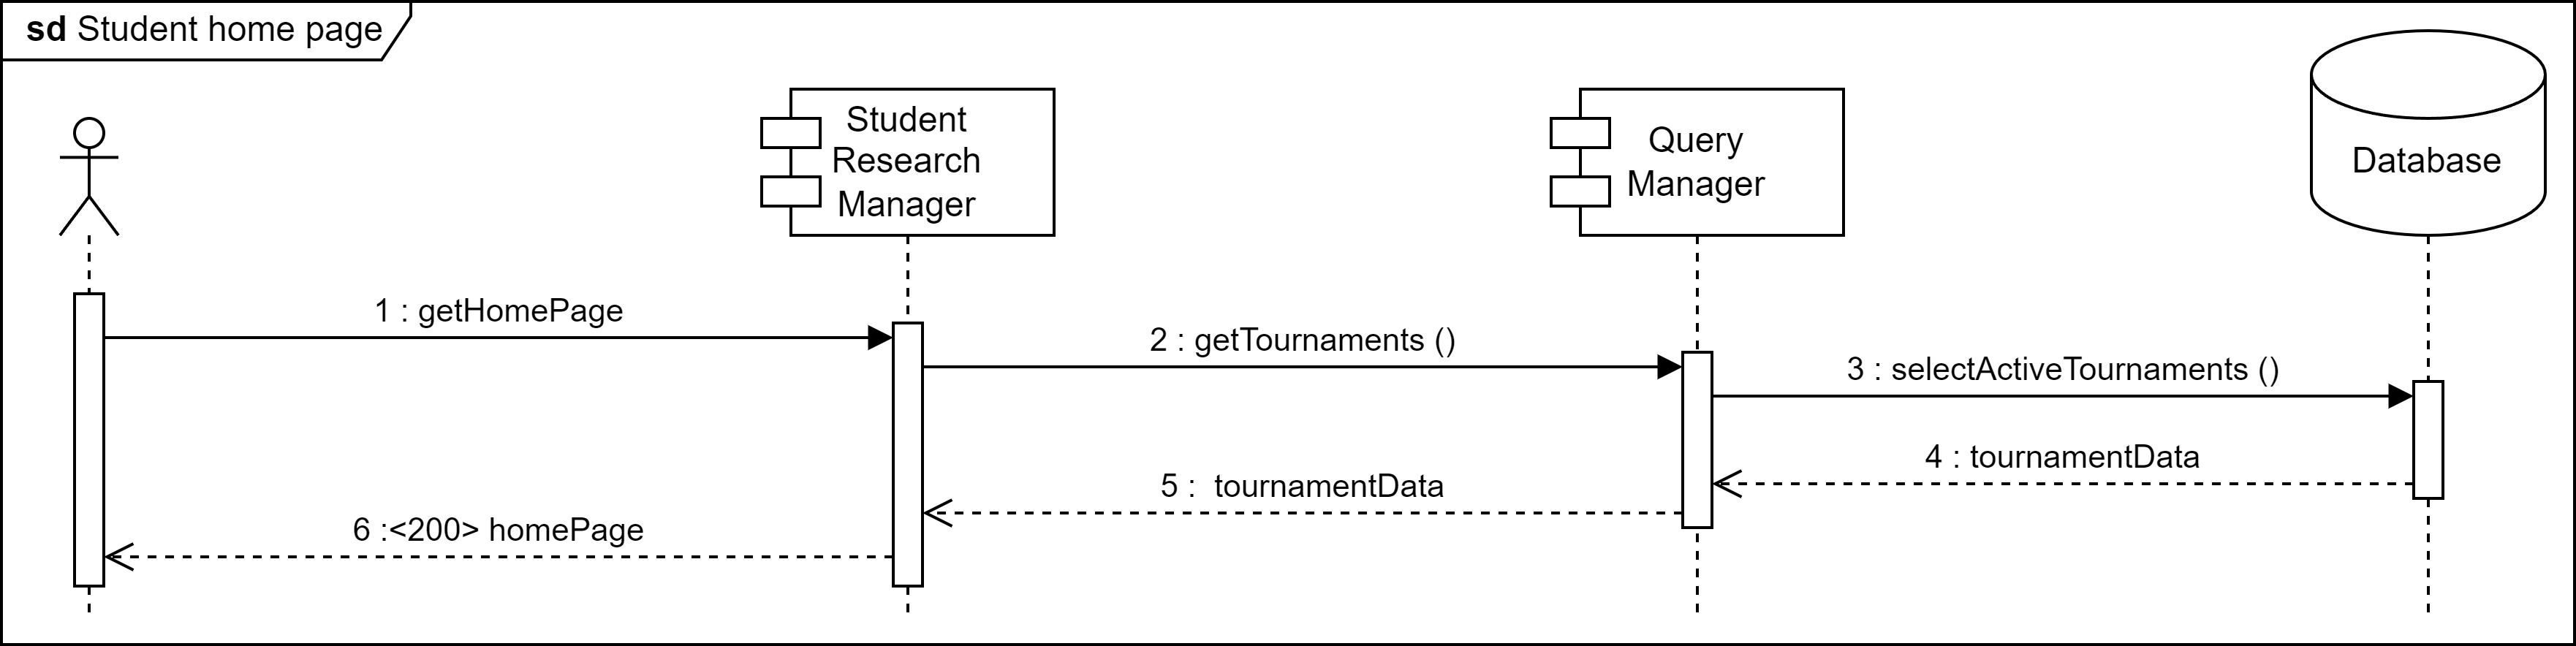
\includegraphics[width=1.0\linewidth]{images/shprv.png}
    \end{figure}

    \paragraph*{Student join tournament}
    In this case the actor is a registered student that wants to join a tournament. 
    The student requests the home page and then select the desired tournament. 
    After clicking the join button the system return the consequence of the action (enrolled or not). 
    \begin{figure}[H]
        \centering
        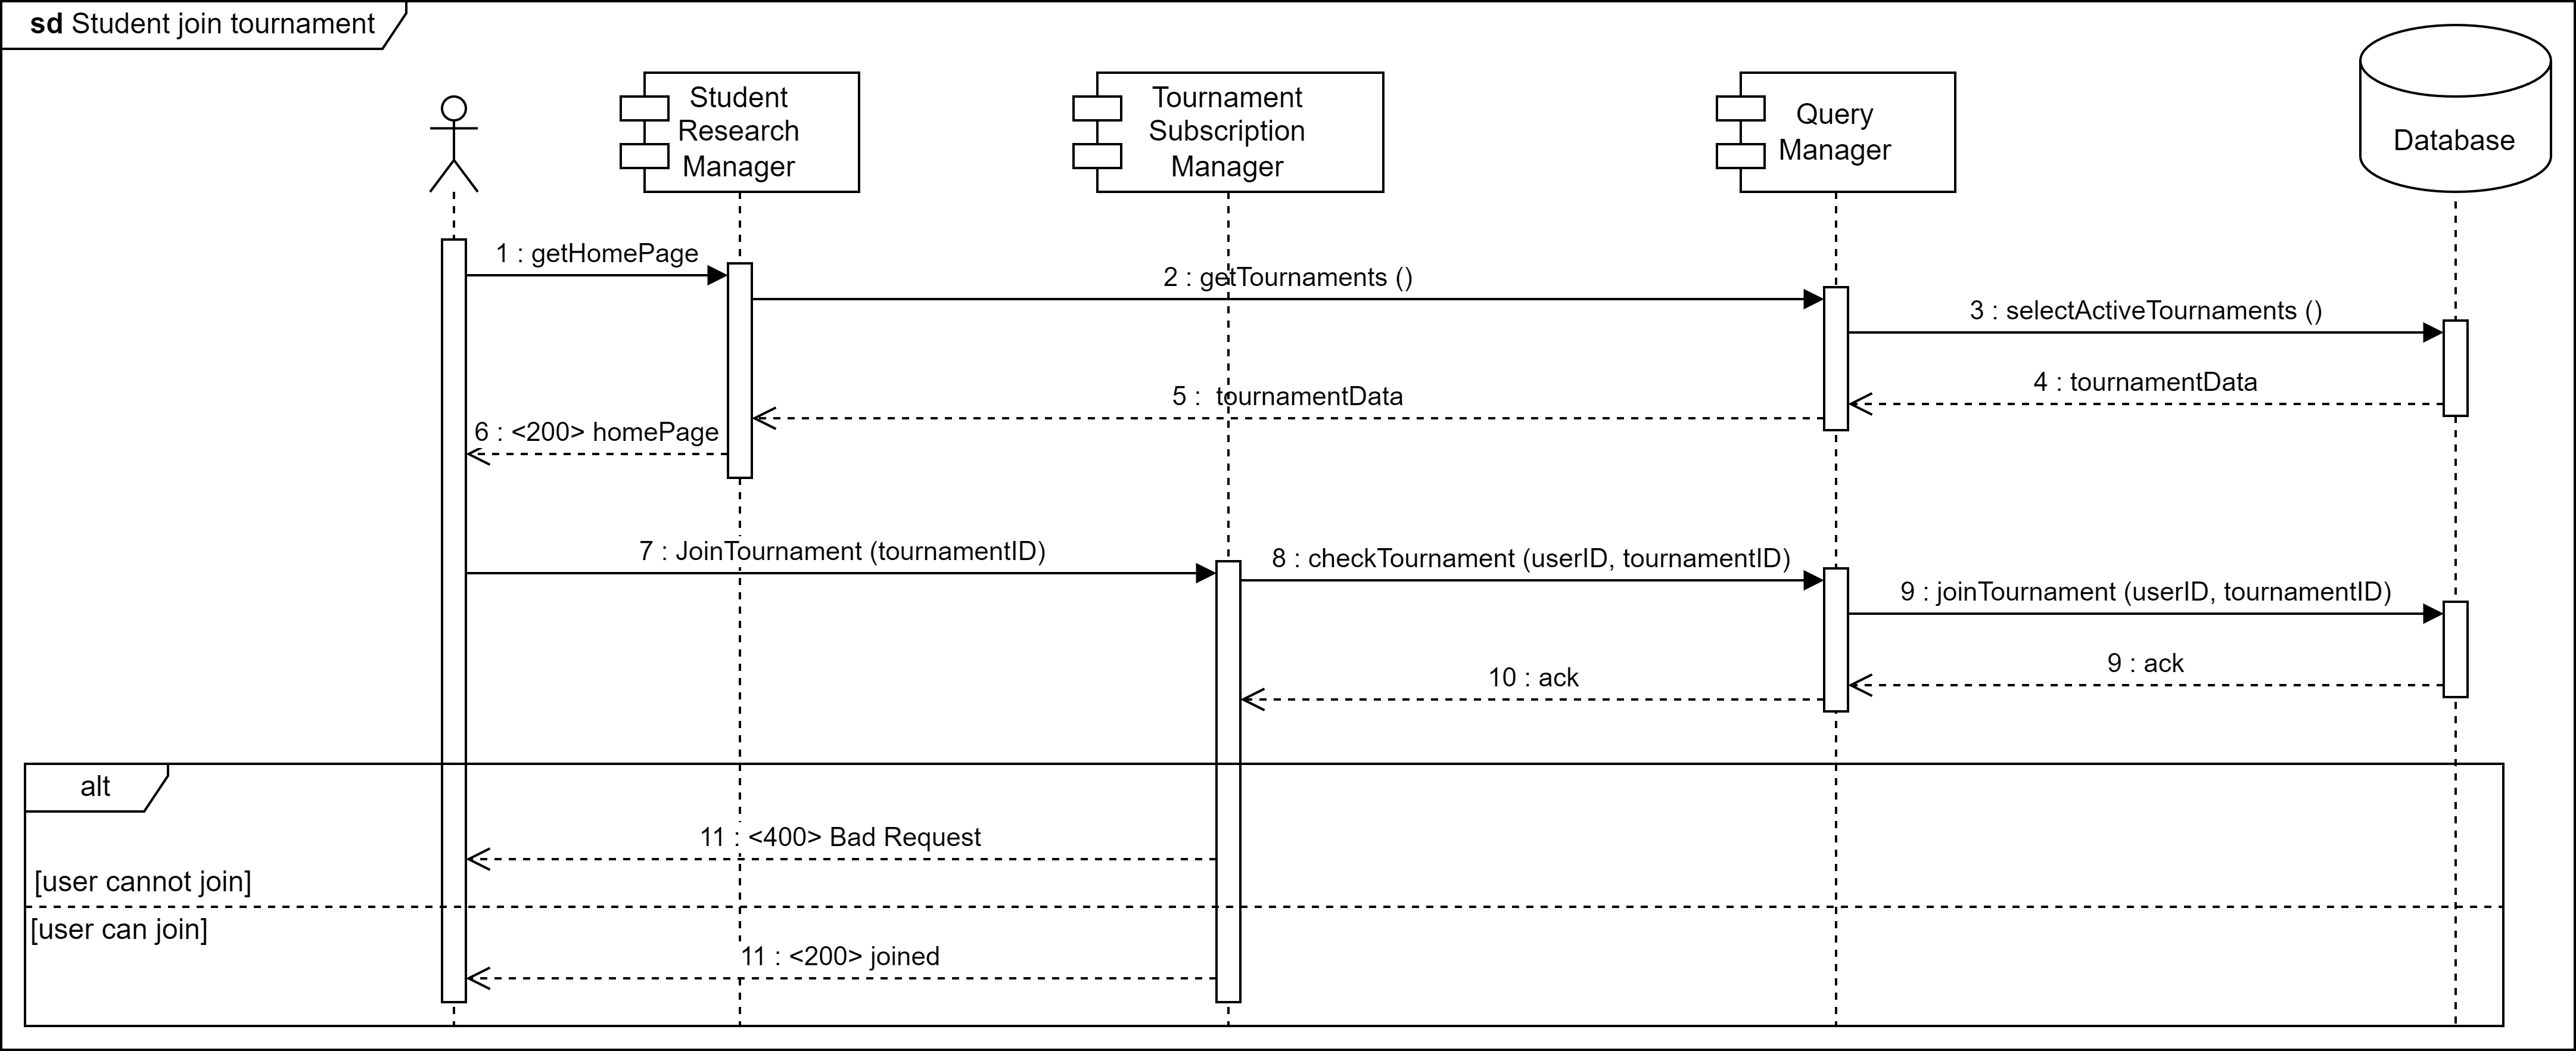
\includegraphics[width=1.0\linewidth]{images/sjtrv.png}
    \end{figure}

    \paragraph*{Student search tournament}
    In this case the actor is a registered student that wants to search for a specific tournament based on a keyword. 
    After accessing the search page the student can finally search the desired tournament. 
    The system returns all the tournaments linked with the searched keyword or a null list if no tournament match the requirements. 
    \begin{figure}[H]
        \centering
        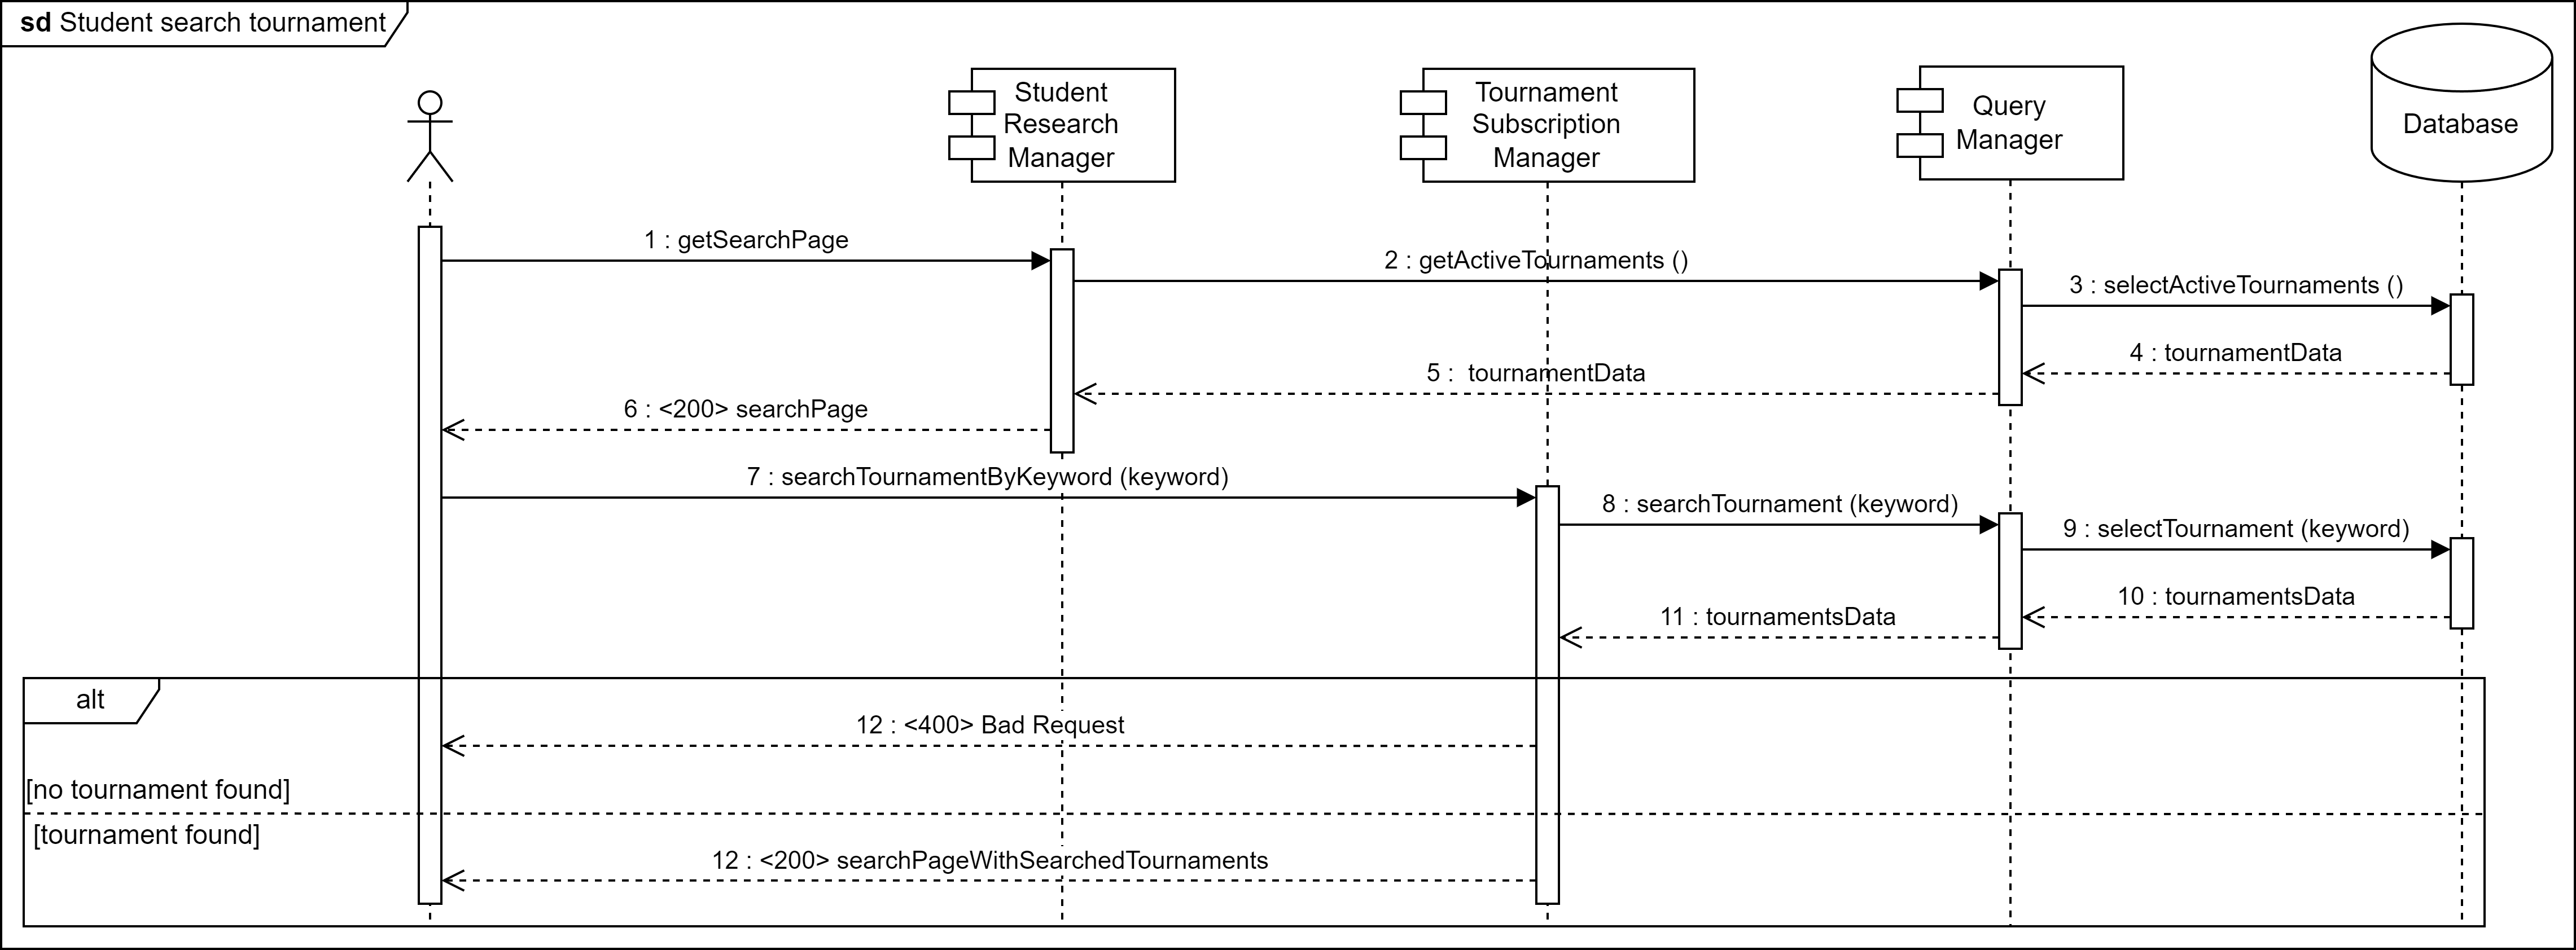
\includegraphics[width=1.0\linewidth]{images/sstrv.png}
    \end{figure}

    \paragraph*{Student join battle}
    In this case the actor is a registered student that wants to join a battle within a tournament in which he is enrolled. 
    After accessing the tournament details page the user clicks on the button to join the battle alone or in a team. 
    If the user is allowed to do the desired enrollment he can finally join the battle. 
    \begin{figure}[H]
        \centering
        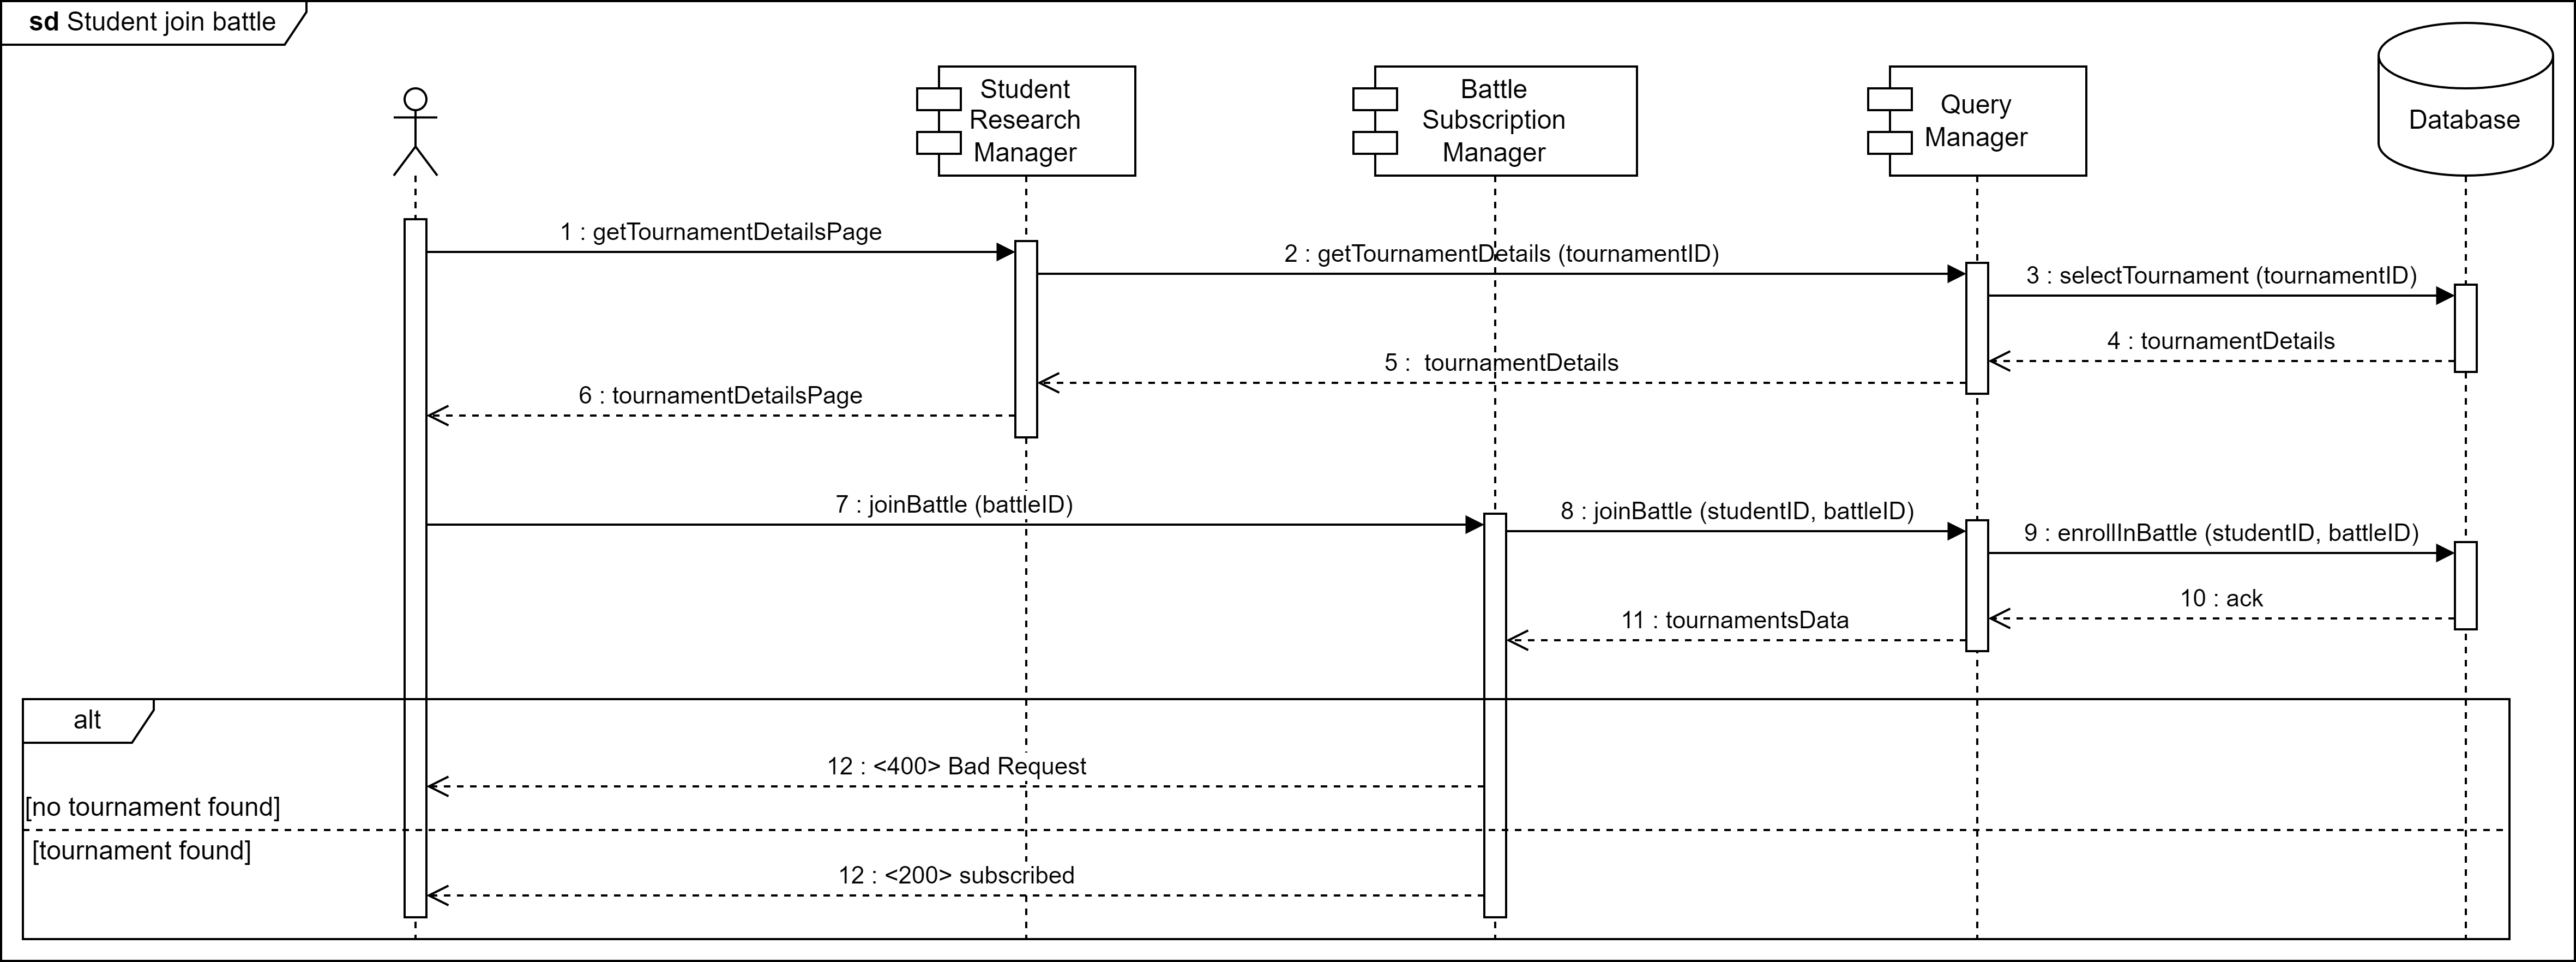
\includegraphics[width=1.0\linewidth]{images/sjbrv.png}
    \end{figure}

    \paragraph*{User checks tournament leaderboard}
    In this case the user is a registered student that wants to check the leaderboard of a tournament. 
    After accessing the enrolled page and consequently the tournament details page the student can access the leaderboard page of the selected tournament. 
    \begin{figure}[H]
        \centering
        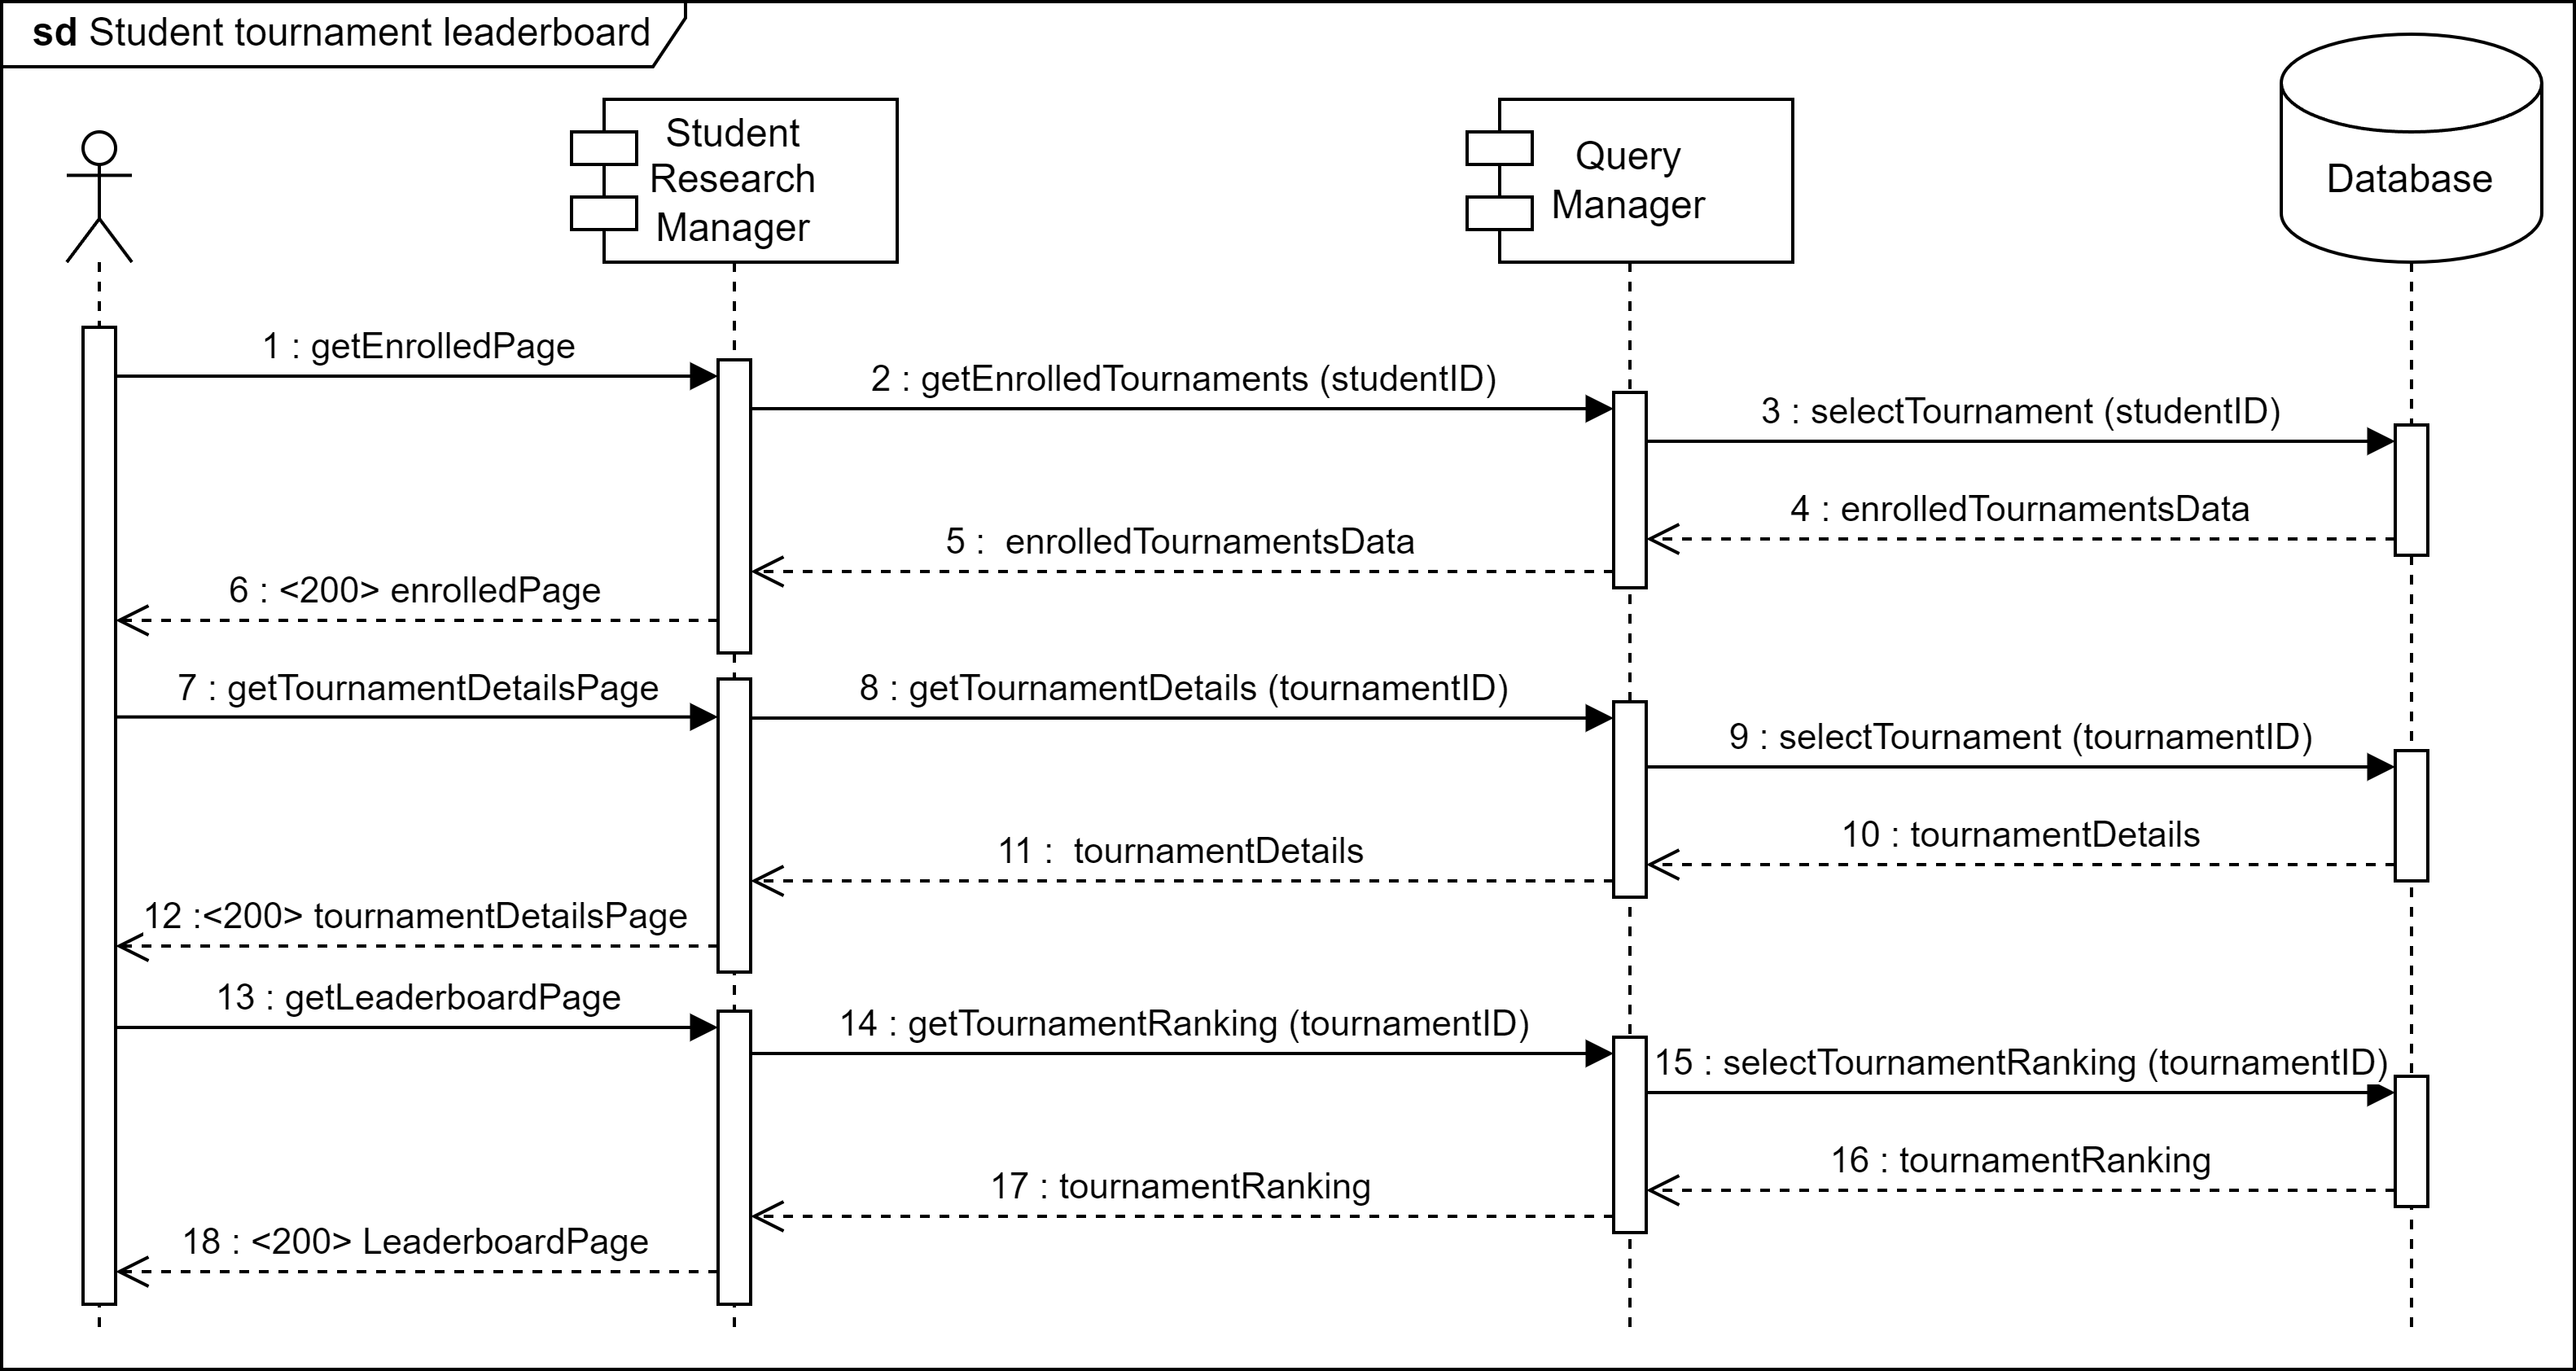
\includegraphics[width=1.0\linewidth]{images/stlrv.png}
    \end{figure}

    \paragraph*{User checks battle leaderboard}
    In this case the user is a registered student that wants to check the leaderboard of a tournament. 
    After accessing the enrolled page and consequently the tournament details page the student can access the leaderboard page of the selected tournament. 
    After this he can click on the button linked to the desired battle within the selected tournament. 
    \begin{figure}[H]
        \centering
        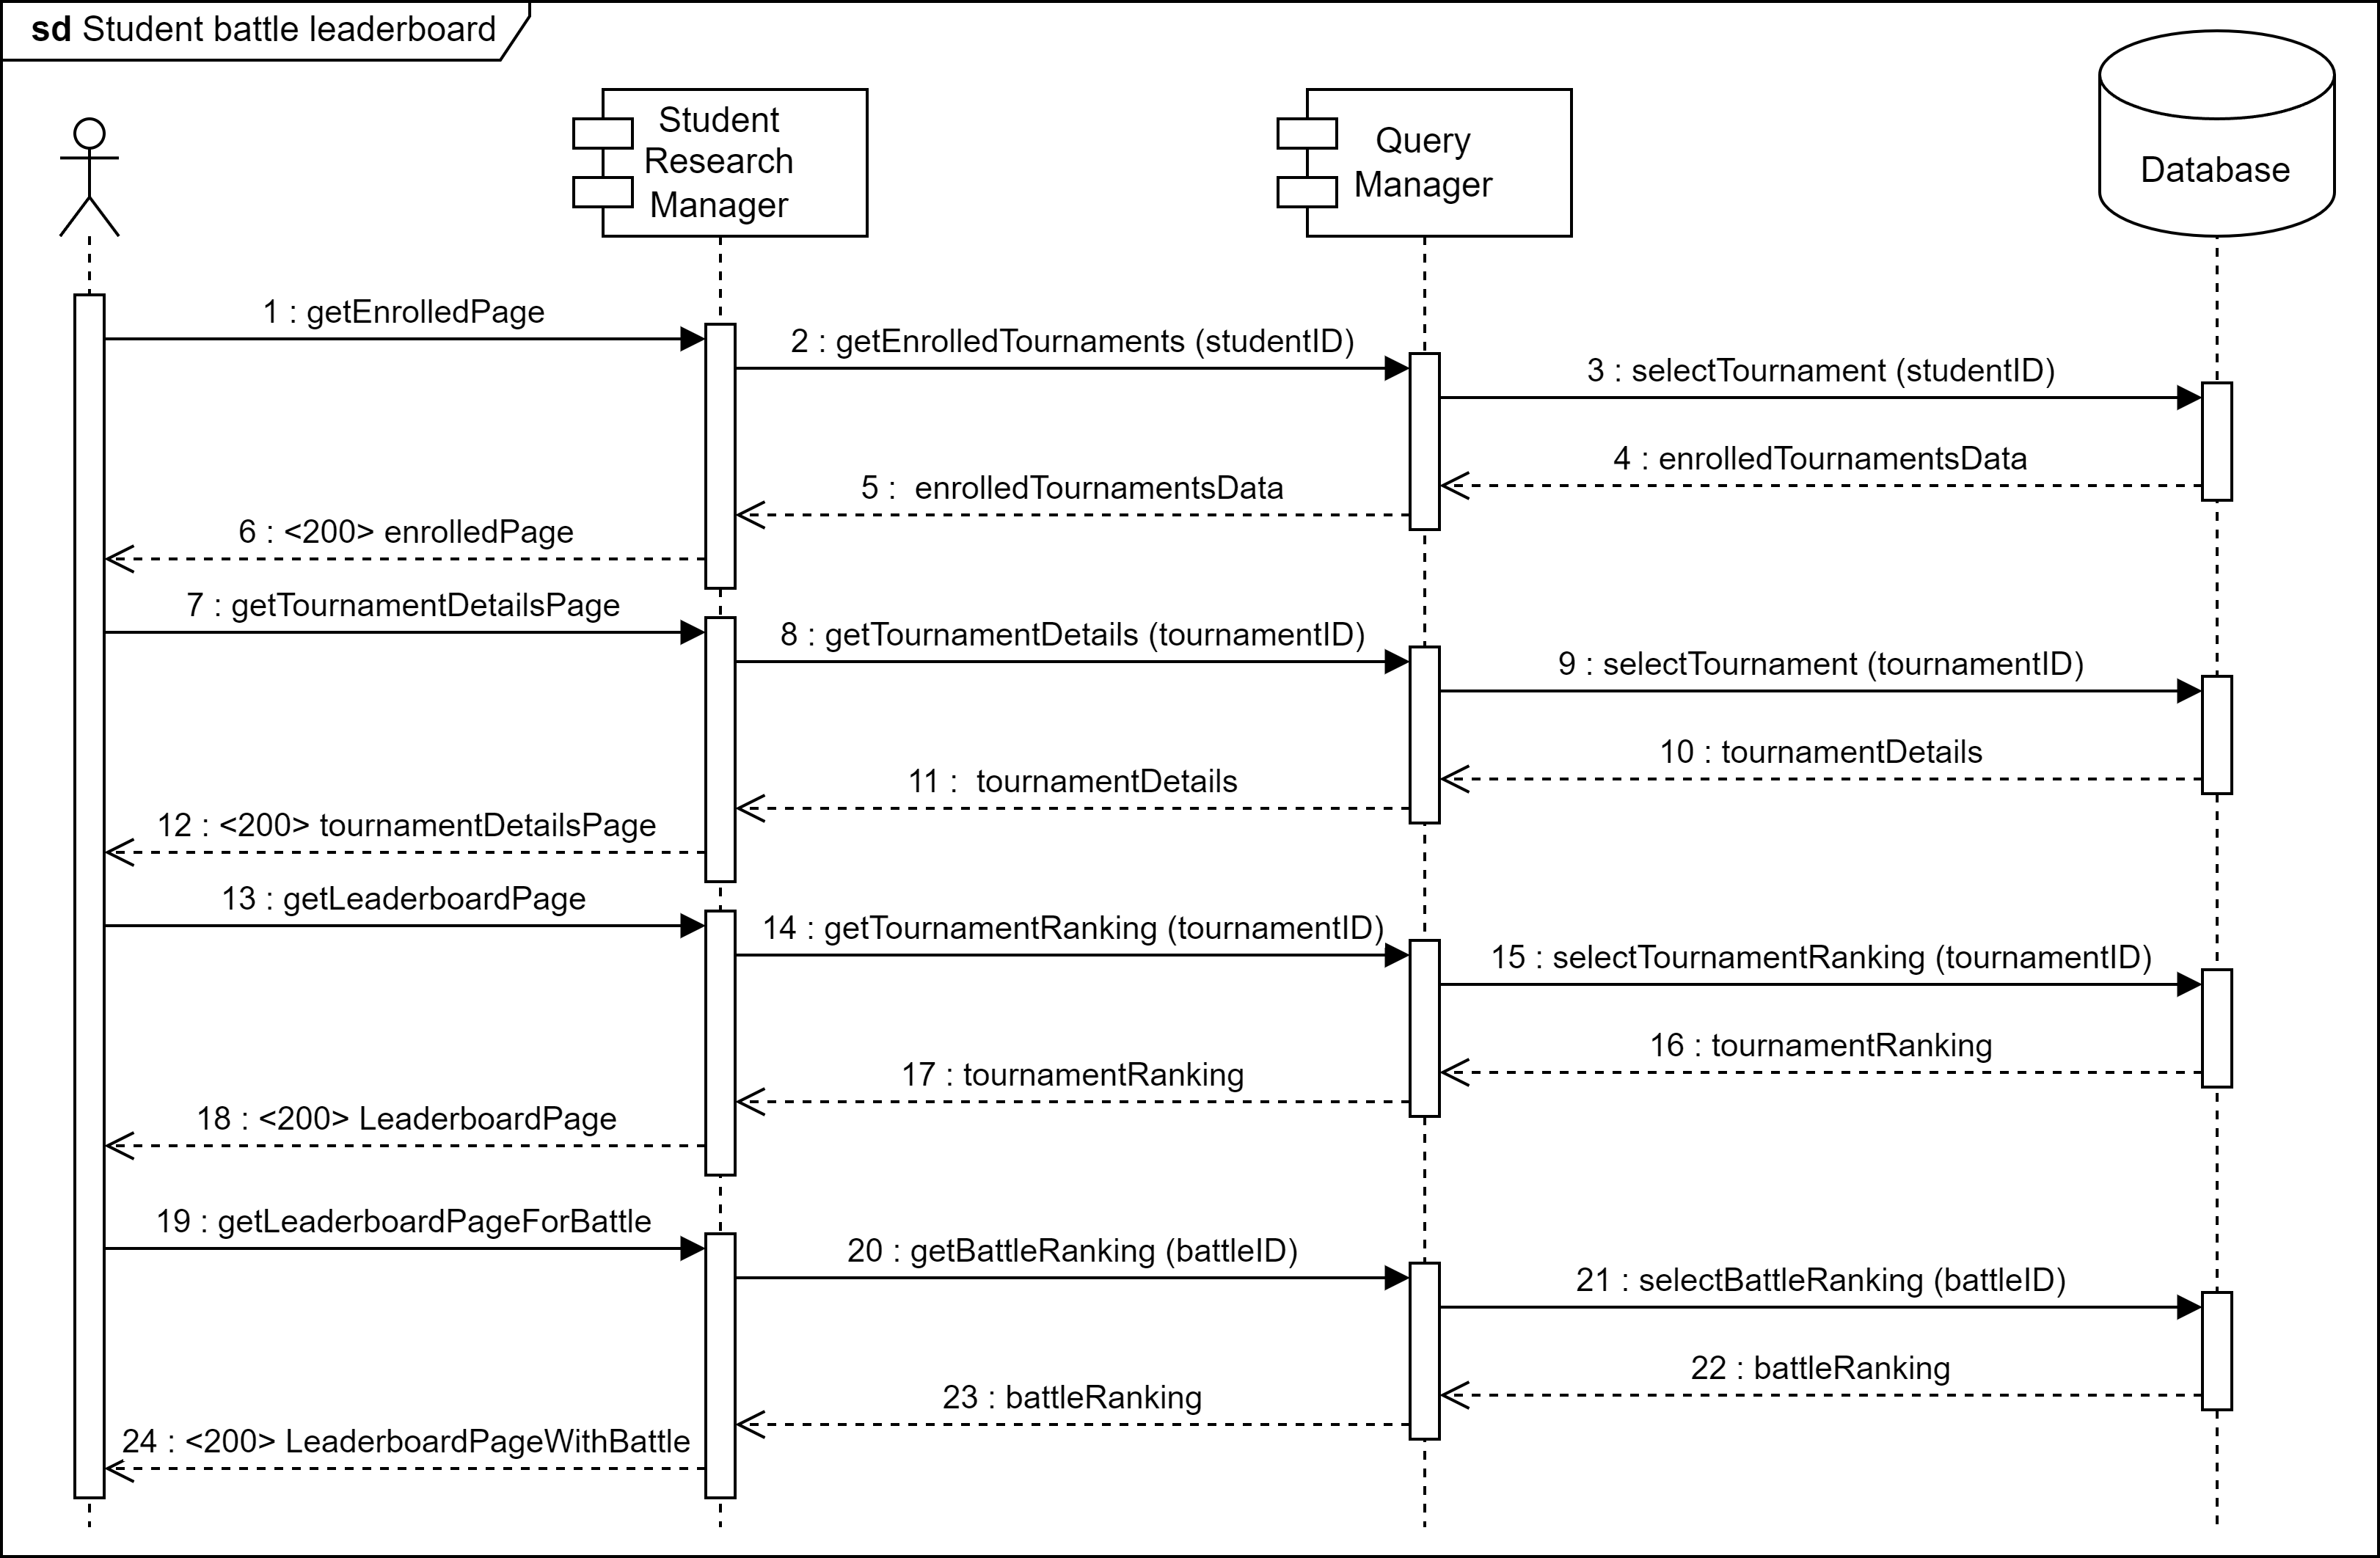
\includegraphics[width=1.0\linewidth]{images/sblrv.png}
    \end{figure}

    \subsection{Educator's runtime view}
    In this section we list all possible actions for the educator along with the runtime view associated with each one. 
    \paragraph*{Educator signup}
    In this case the actor is an unregistered educator that is trying to sign up in the system.
    After accessing the corresponding page the educator submits all the required information to the educator account manager component that checks the data. 
    If the user is not already register it creates a new educator after the email verification. 
    \begin{figure}[H]
        \centering
        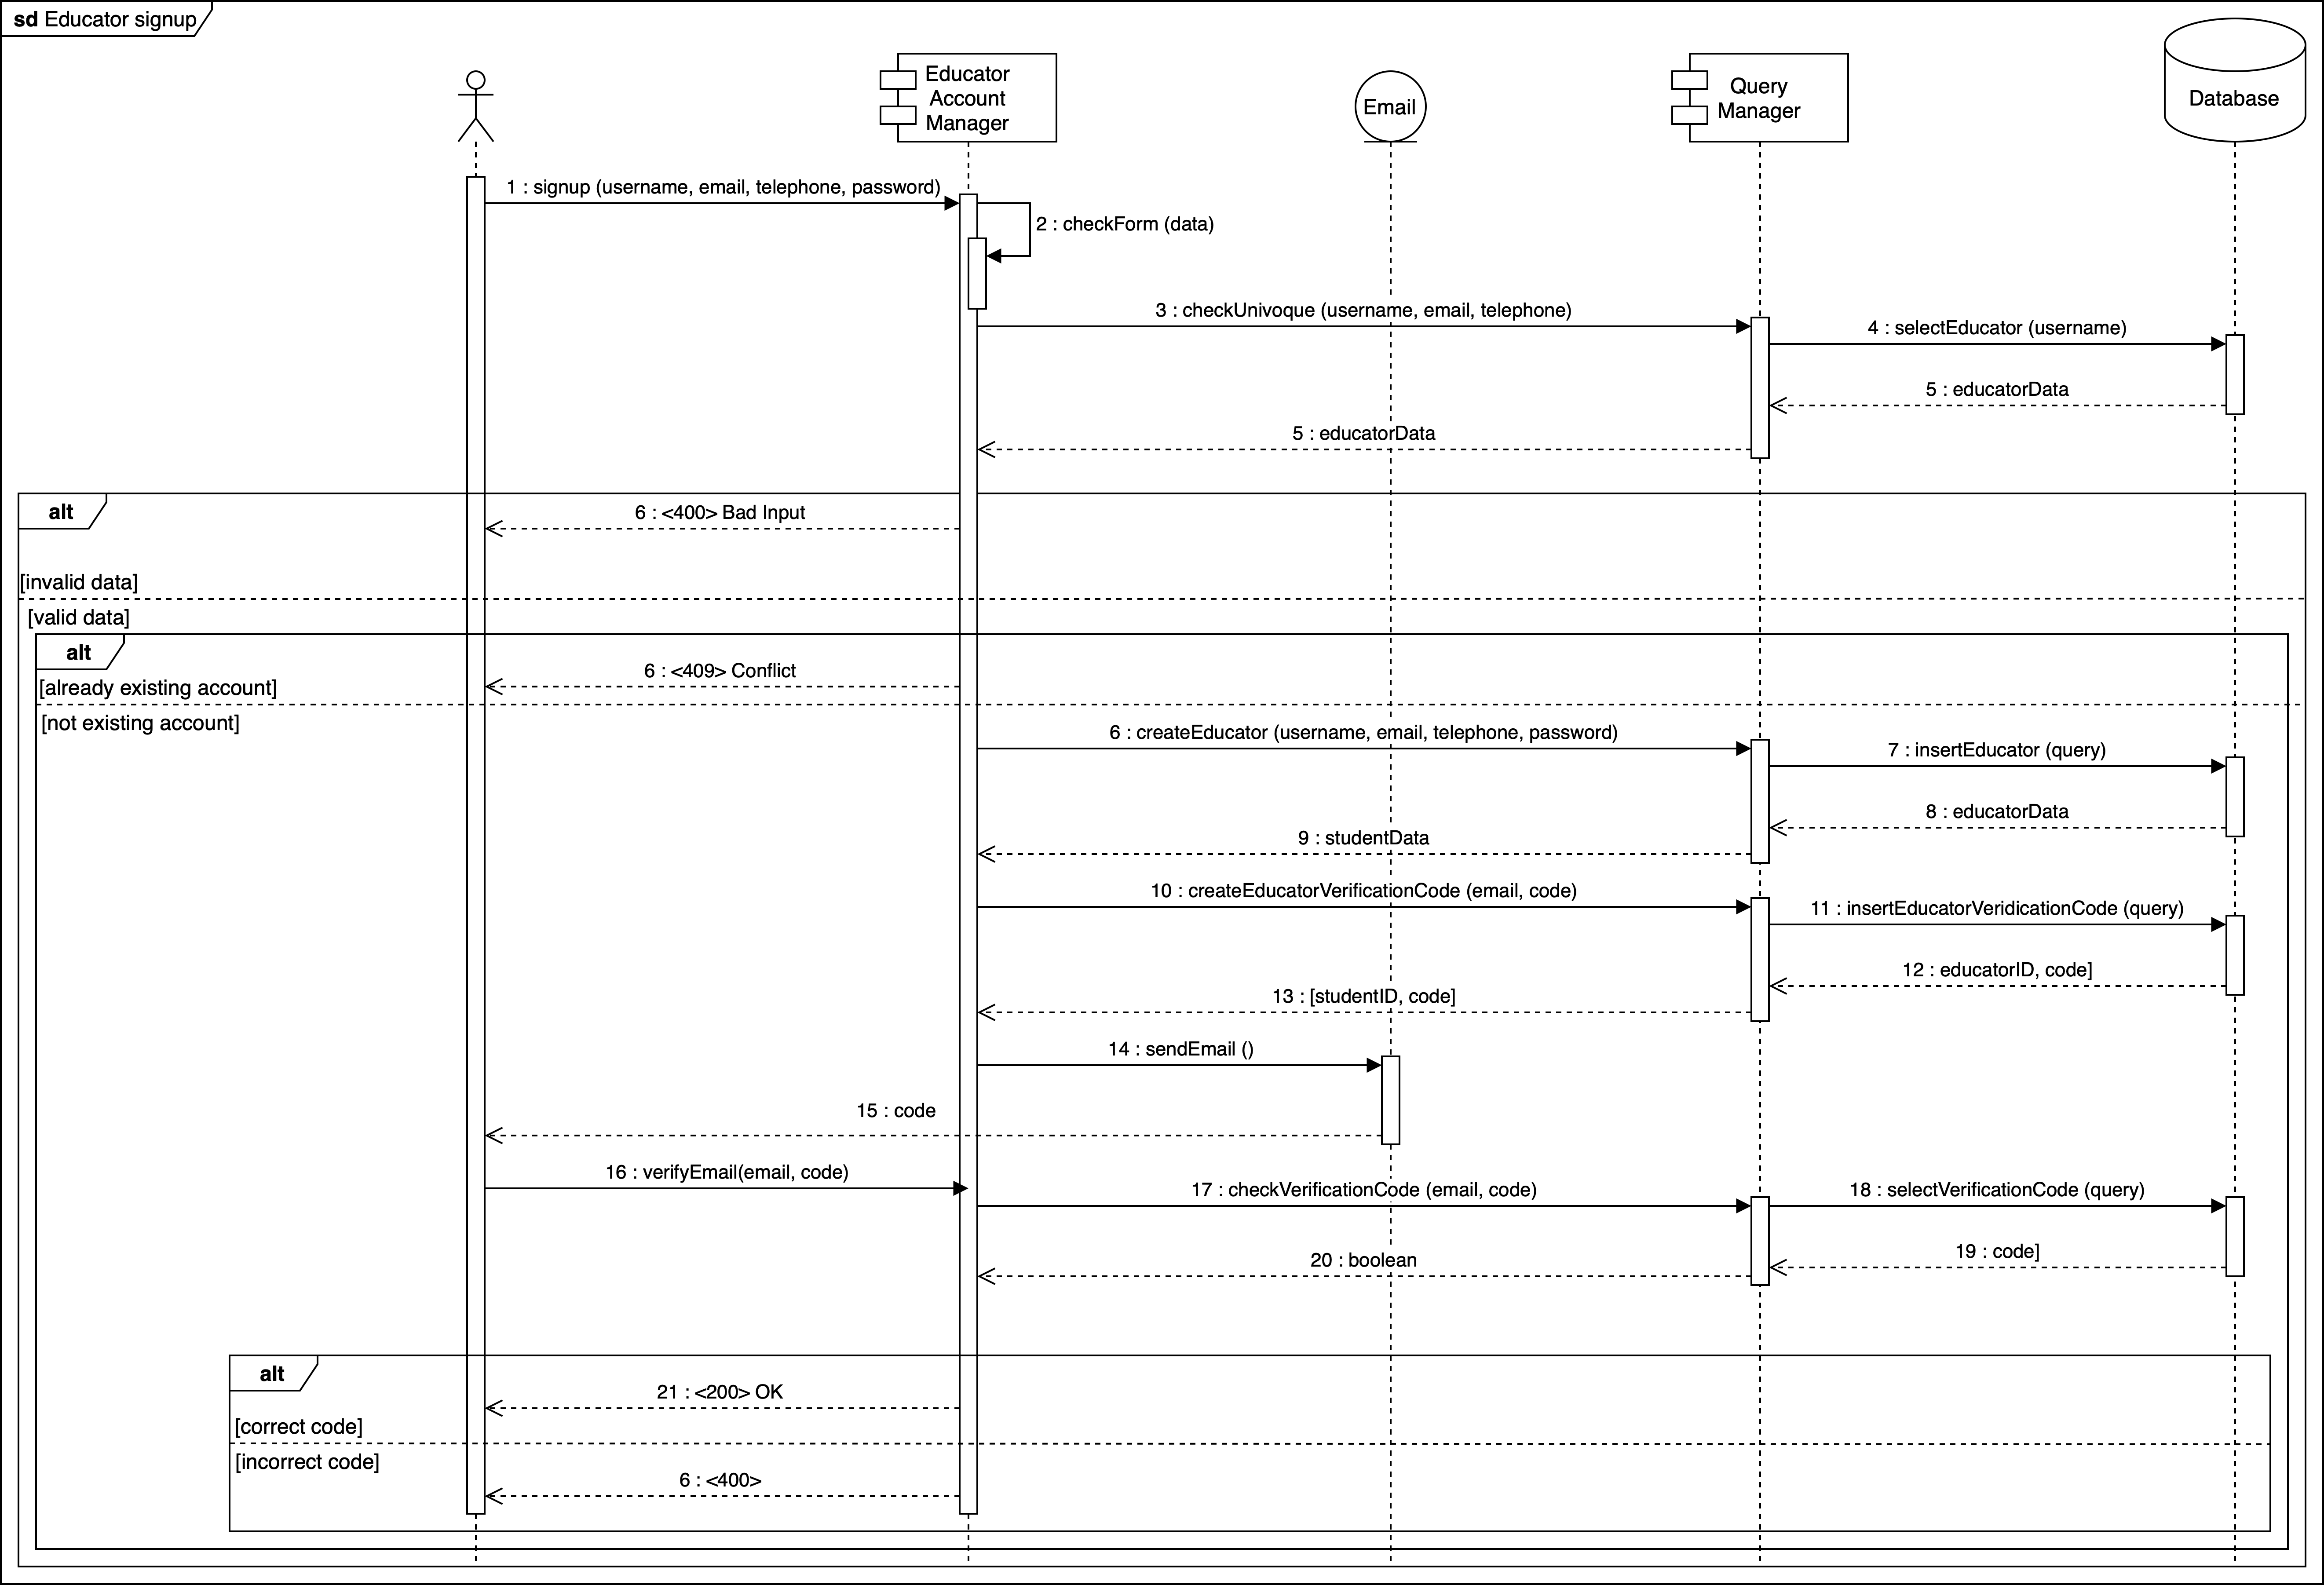
\includegraphics[width=1.0\linewidth]{images/esrv.png}
    \end{figure}

    \paragraph*{Educator log in}
    \begin{figure}[H]
        \centering
        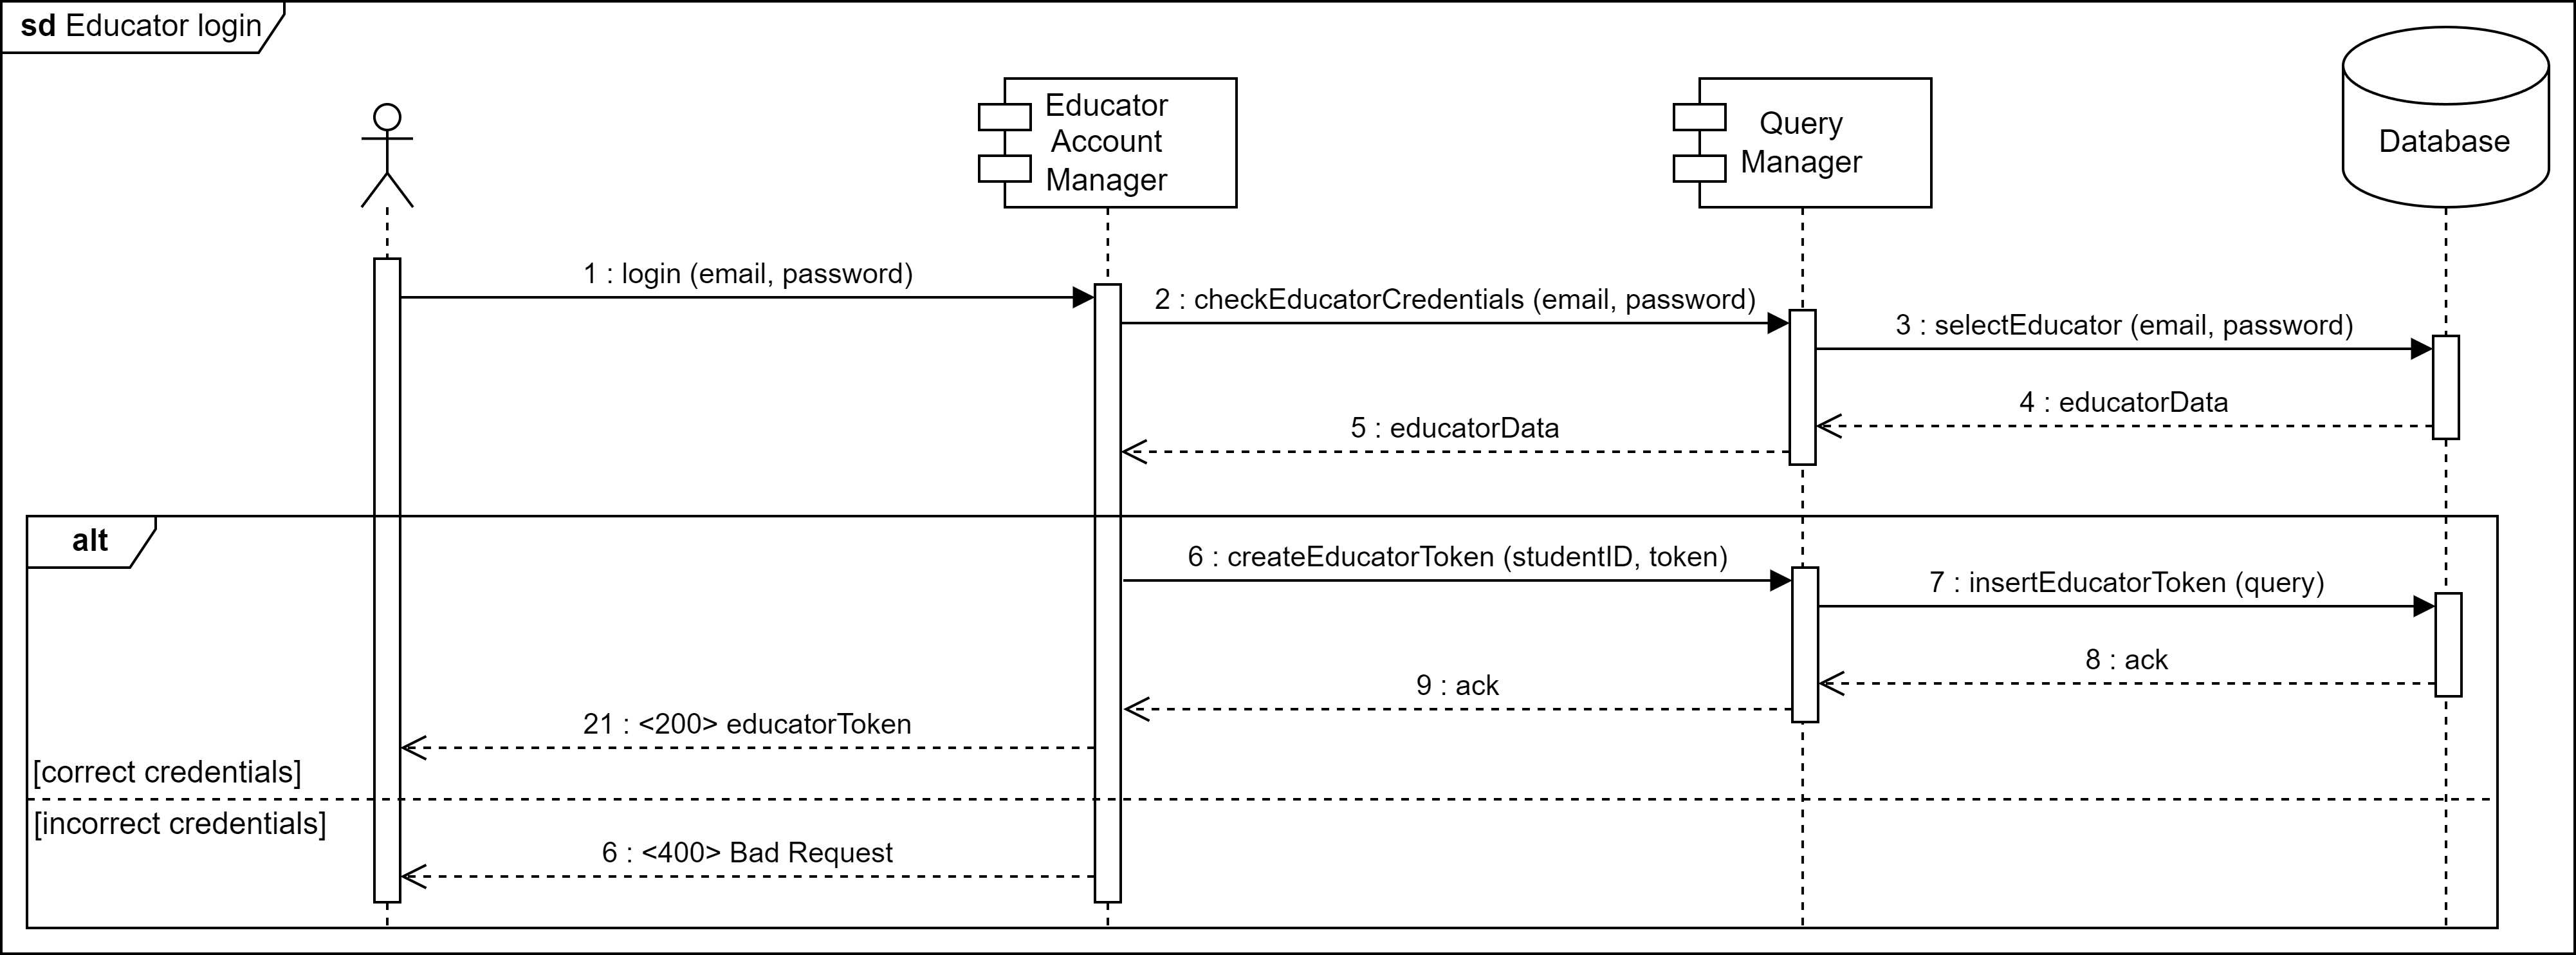
\includegraphics[width=1.0\linewidth]{images/elirv.png}
    \end{figure}
    In this case the actor is a registered educator that wants to log in into the system. 
    After accessing the corresponding page the educator submits all the required information to the educator account manager component that checks the data. 
    If the inserted data are correct the educator can access all his possible actions. 

    \paragraph*{Educator profile}
    In this case the actor is a registered educator that wants to check his own profile. 
    The educator profile manager retrieves all the data linked to the educator and returns the complete page to the educator. 
    \begin{figure}[H]
        \centering
        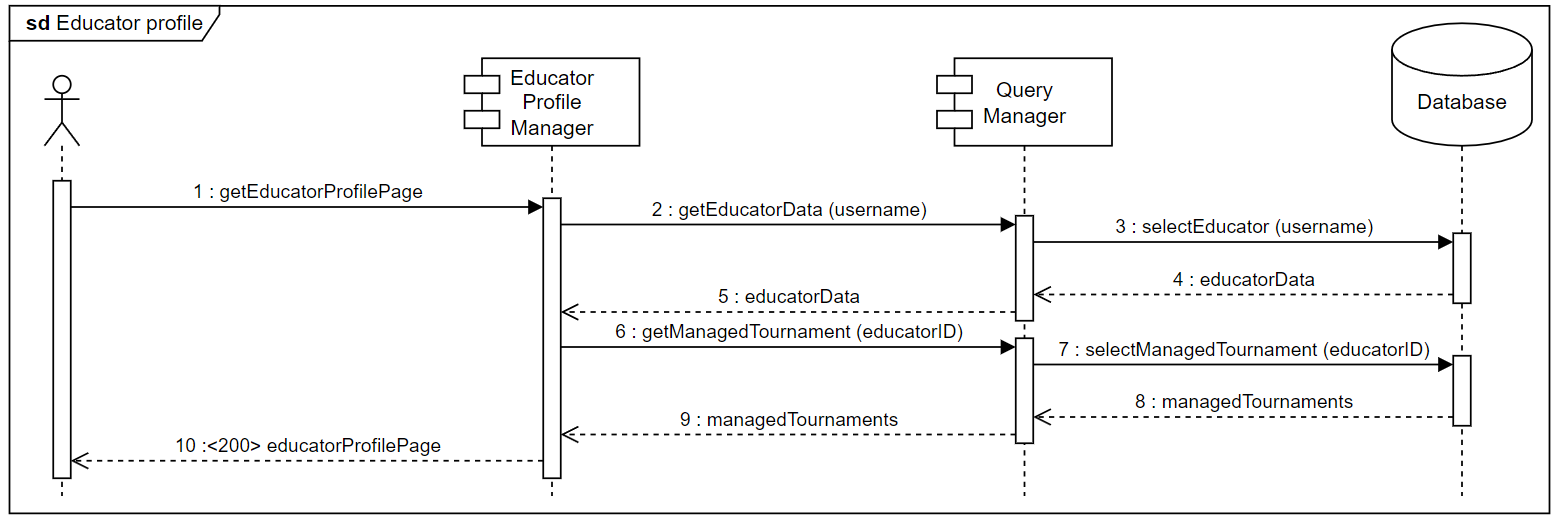
\includegraphics[width=1.0\linewidth]{images/eprv.png}
    \end{figure}

    \paragraph*{Educator home page}
    In this case the actor is a registered educator that wants to access the home page. 
    The educator research manager retrieves all the active tournaments from the database and return the home page with some tournaments. 
    \begin{figure}[H]
        \centering
        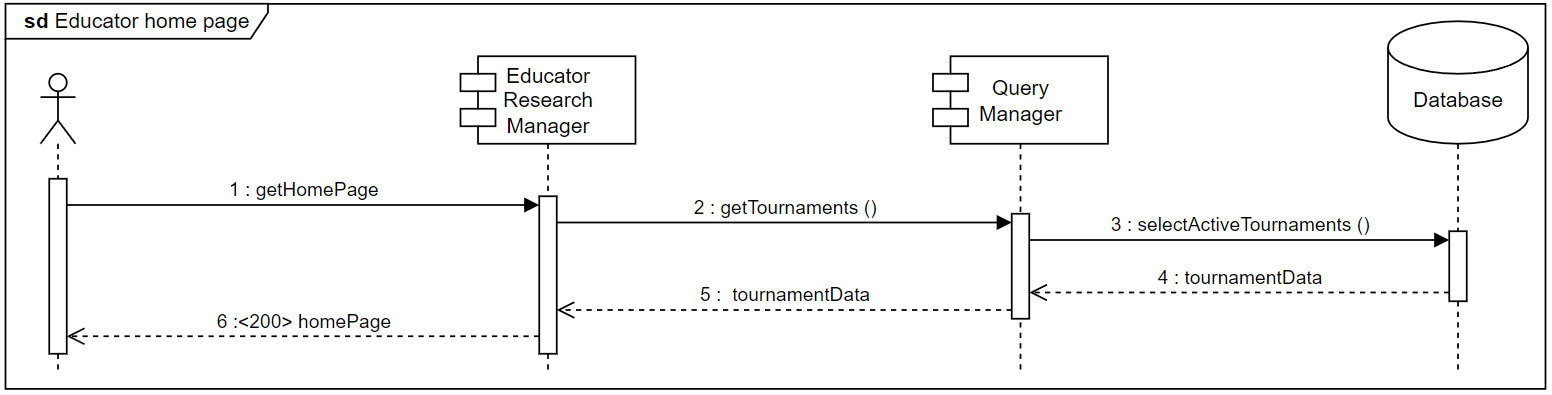
\includegraphics[width=1.0\linewidth]{images/ehprv.png}
    \end{figure}

    \paragraph*{Educator search tournament}
    In this case the actor is a registered educator that wants to search for a specific tournament based on a keyword. 
    After accessing the search page the educator can finally search the desired tournament. 
    The system returns all the tournaments linked with the searched keyword or a null list if no tournament match the requirements. 
    \begin{figure}[H]
        \centering
        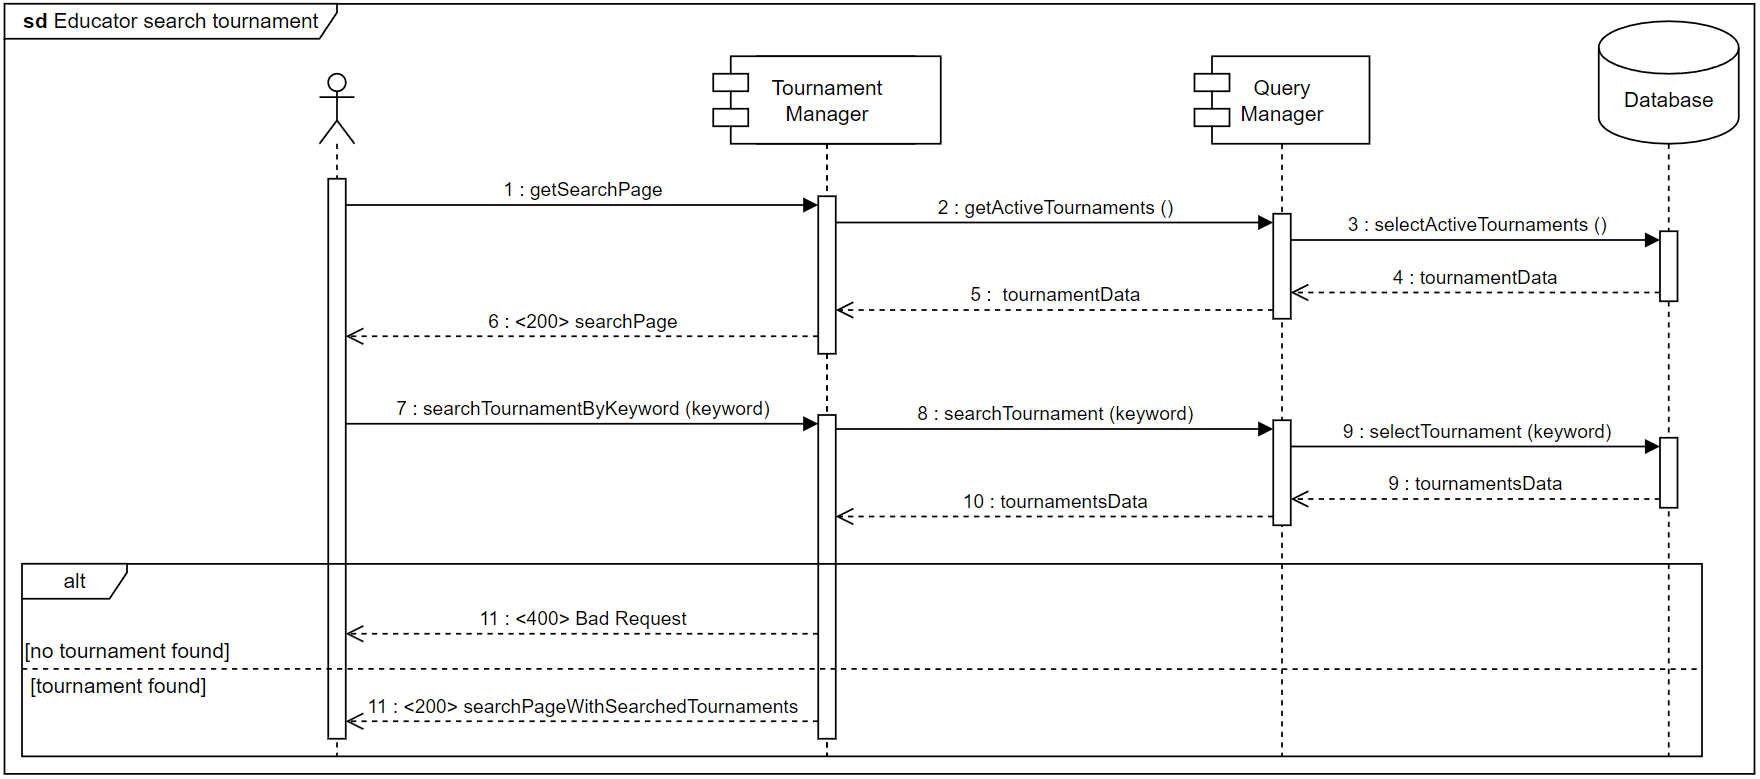
\includegraphics[width=1.0\linewidth]{images/estrv.png}
    \end{figure}

    \paragraph*{Educator create tournament}
    In this case the actor is an educator that wants to create a new tournament. 
    After accessing the create tournament page and compiling all the requested information he submits the data. 
    The system check all information and returns the state of the requested action (the creation of the tournament). 
    \begin{figure}[H]
        \centering
        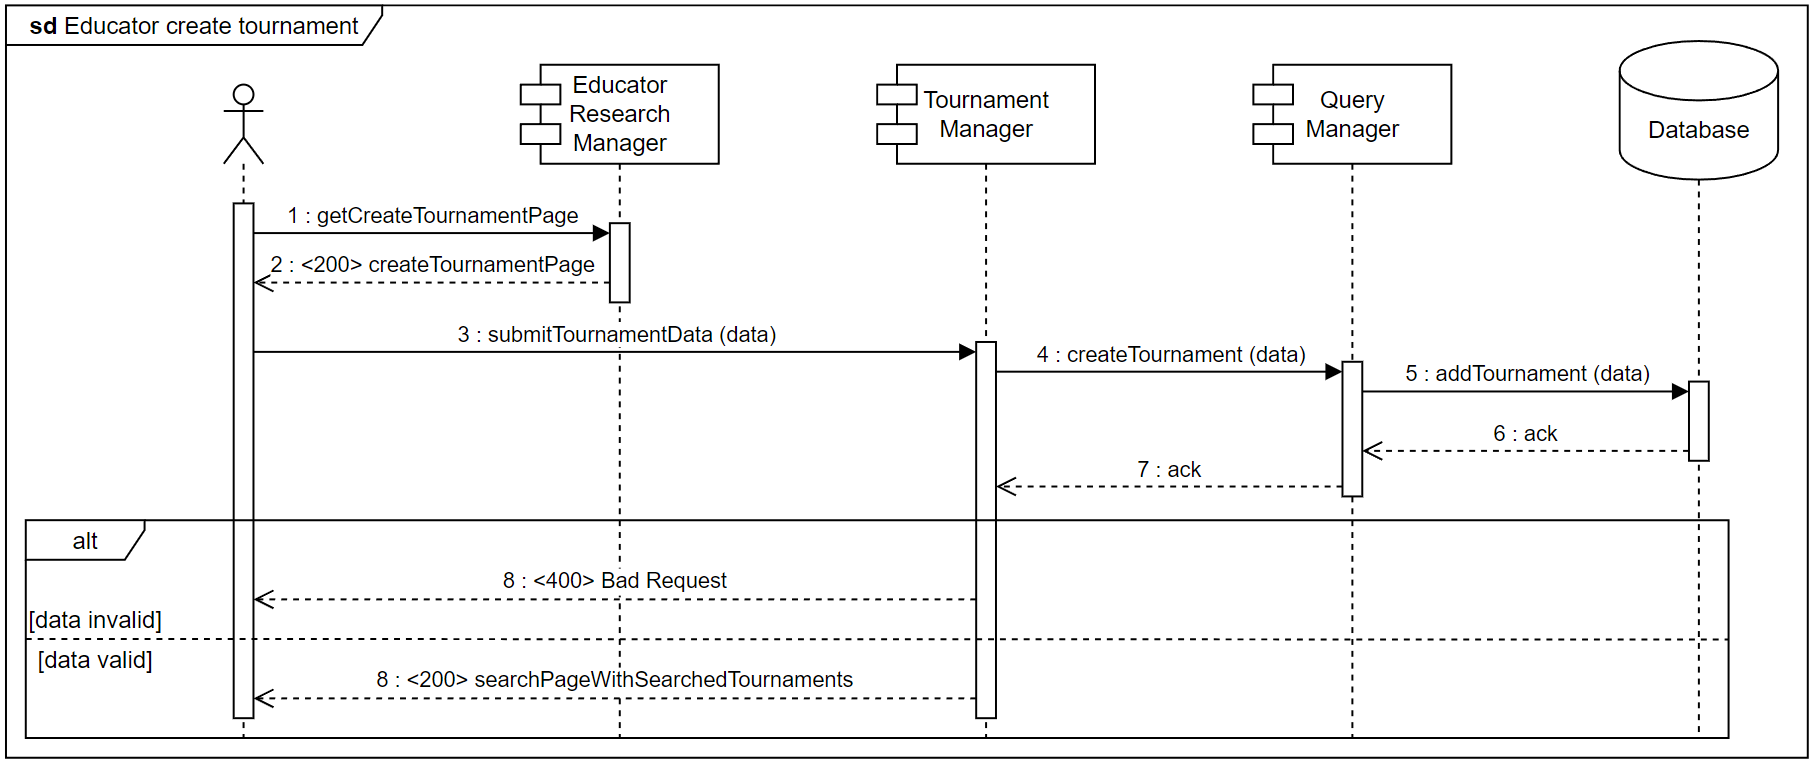
\includegraphics[width=1.0\linewidth]{images/ectrv.png}
    \end{figure}

    \paragraph*{Educator manage tournament}
    In this case the actor is an educator that wants to manage an already existing tournament. 
    After accessing the manage tournament page he clicks on the desired tournament. 
    The system check if the user is allowed to check the tournament and returns the same page with all the details. 
    \begin{figure}[H]
        \centering
        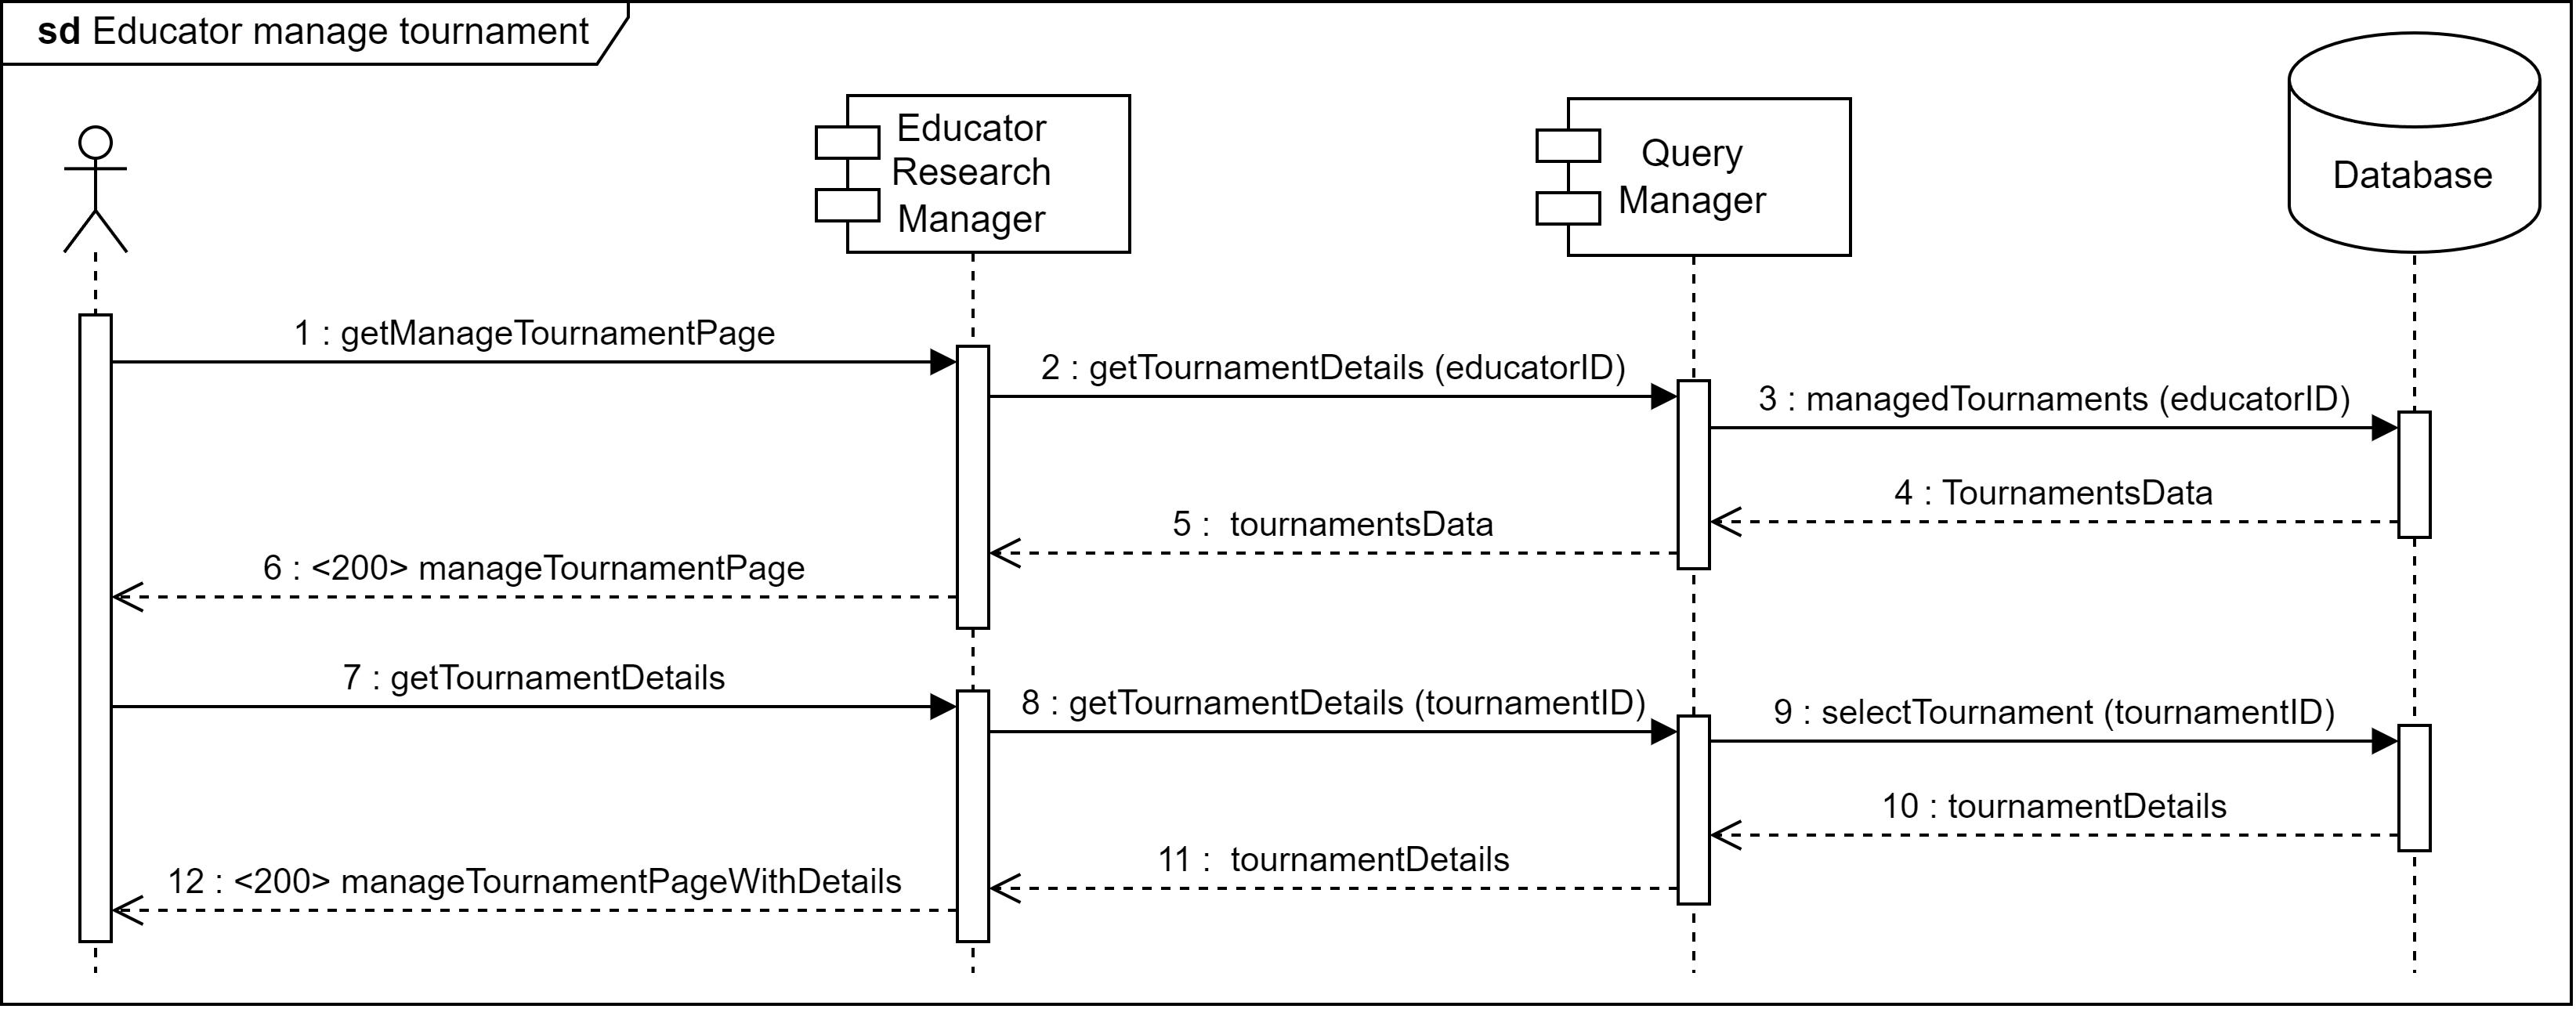
\includegraphics[width=1.0\linewidth]{images/emtrv.png}
    \end{figure}

    \paragraph*{Educator add battle}
    In this case the actor is an educator that wants to manage an already existing tournament by adding a battle. 
    After accessing the manage tournament page he clicks on the desired tournament. 
    The system check if the user is allowed to check the tournament and returns the same page with all the details. 
    Now the educator can finally click on the add button to create a new battle within the tournament. 
    The system return the create battle page, and the educator can finally insert all the information regarding the battle. 
    If all data are correct the system adds the new battle and notifies the educator. 
    \begin{figure}[H]
        \centering
        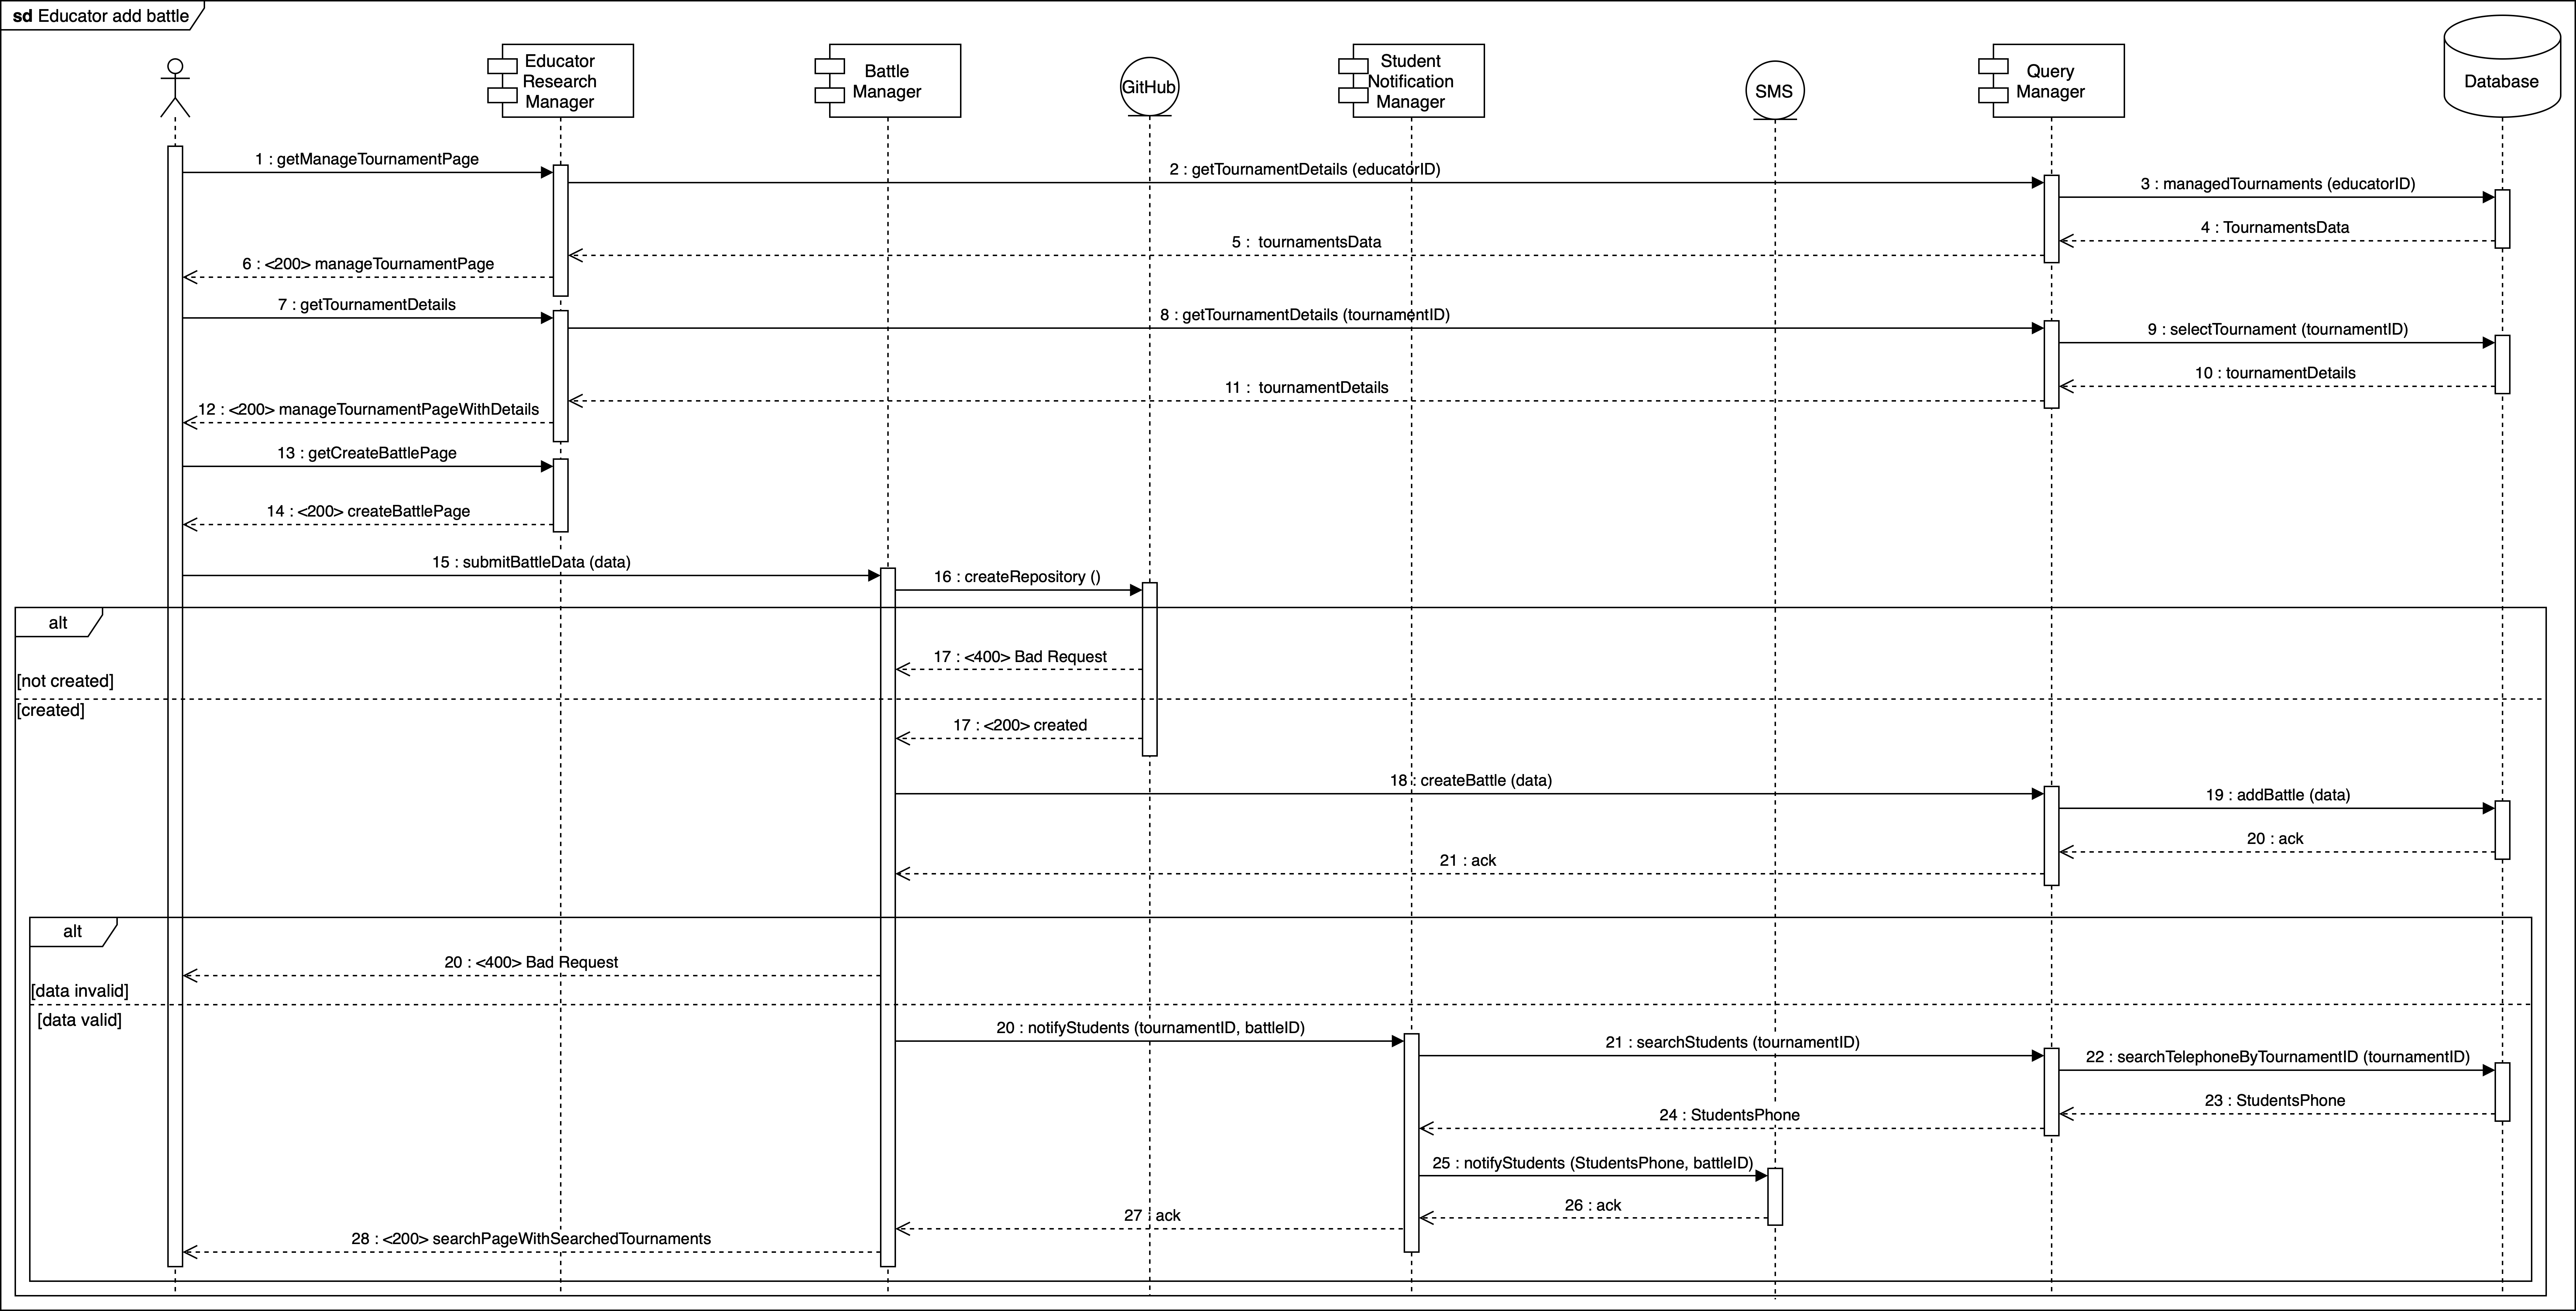
\includegraphics[width=1.0\linewidth]{images/eabrv.png}
    \end{figure}

    \paragraph*{Educator add collaborator}
    In this case the actor is an educator that wants to manage an already existing tournament by adding a collaborator. 
    After accessing the manage tournament page he clicks on the desired tournament. 
    The system check if the user is allowed to check the tournament and returns the same page with all the details. 
    Now the educator can finally click on the add collaborator button to invite other educators. 
    The educator submits the email and the system let him know if the collaborator is invited or not. 
    \begin{figure}[H]
        \centering
        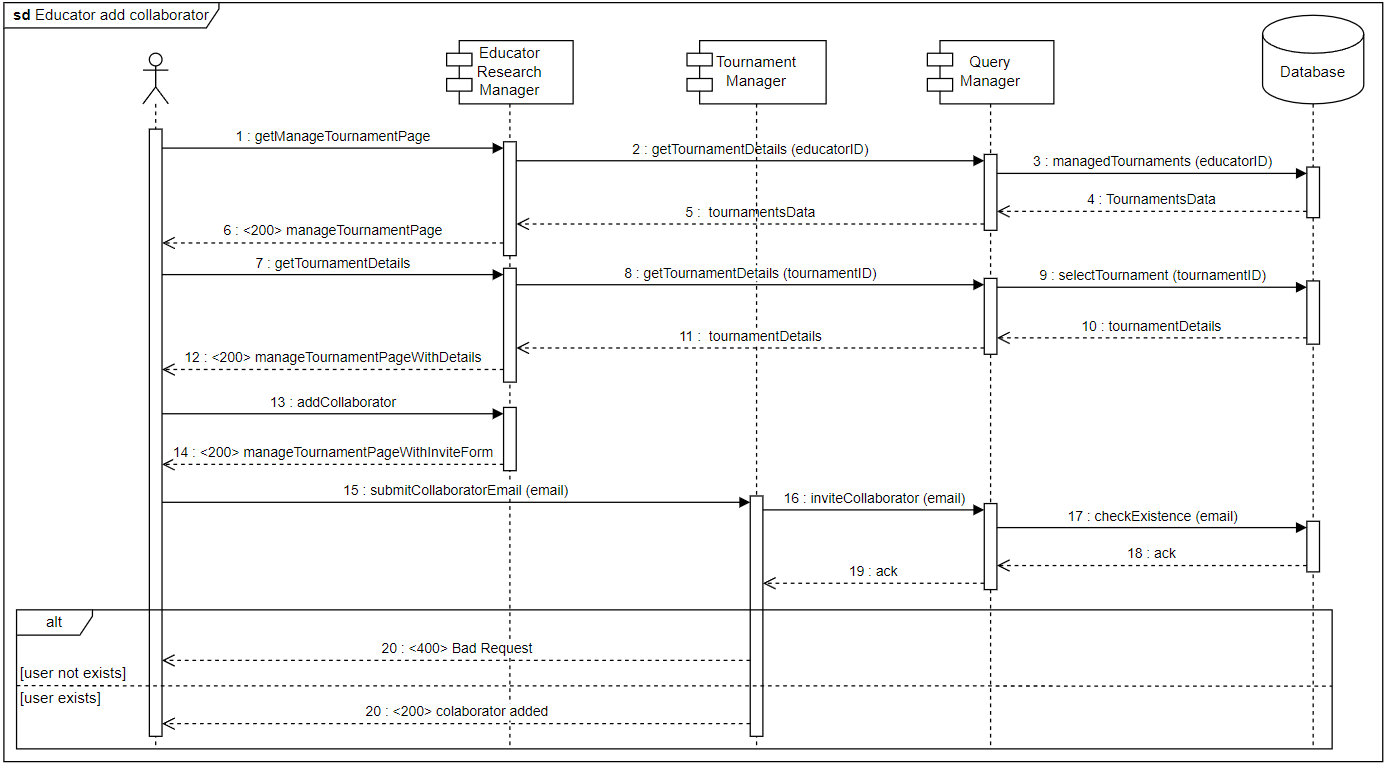
\includegraphics[width=1.0\linewidth]{images/eacrv.png}
    \end{figure}

    \paragraph*{Educator close tournament}
    In this case the actor is an educator that wants to manage an already existing tournament by closing it. 
    After accessing the manage tournament page he clicks on the desired tournament. 
    The system check if the user is allowed to check the tournament and returns the same page with all the details. 
    Now the educator can finally click on the close button. 
    The system notifies the educator on the status of the action. 
    \begin{figure}[H]
        \centering
        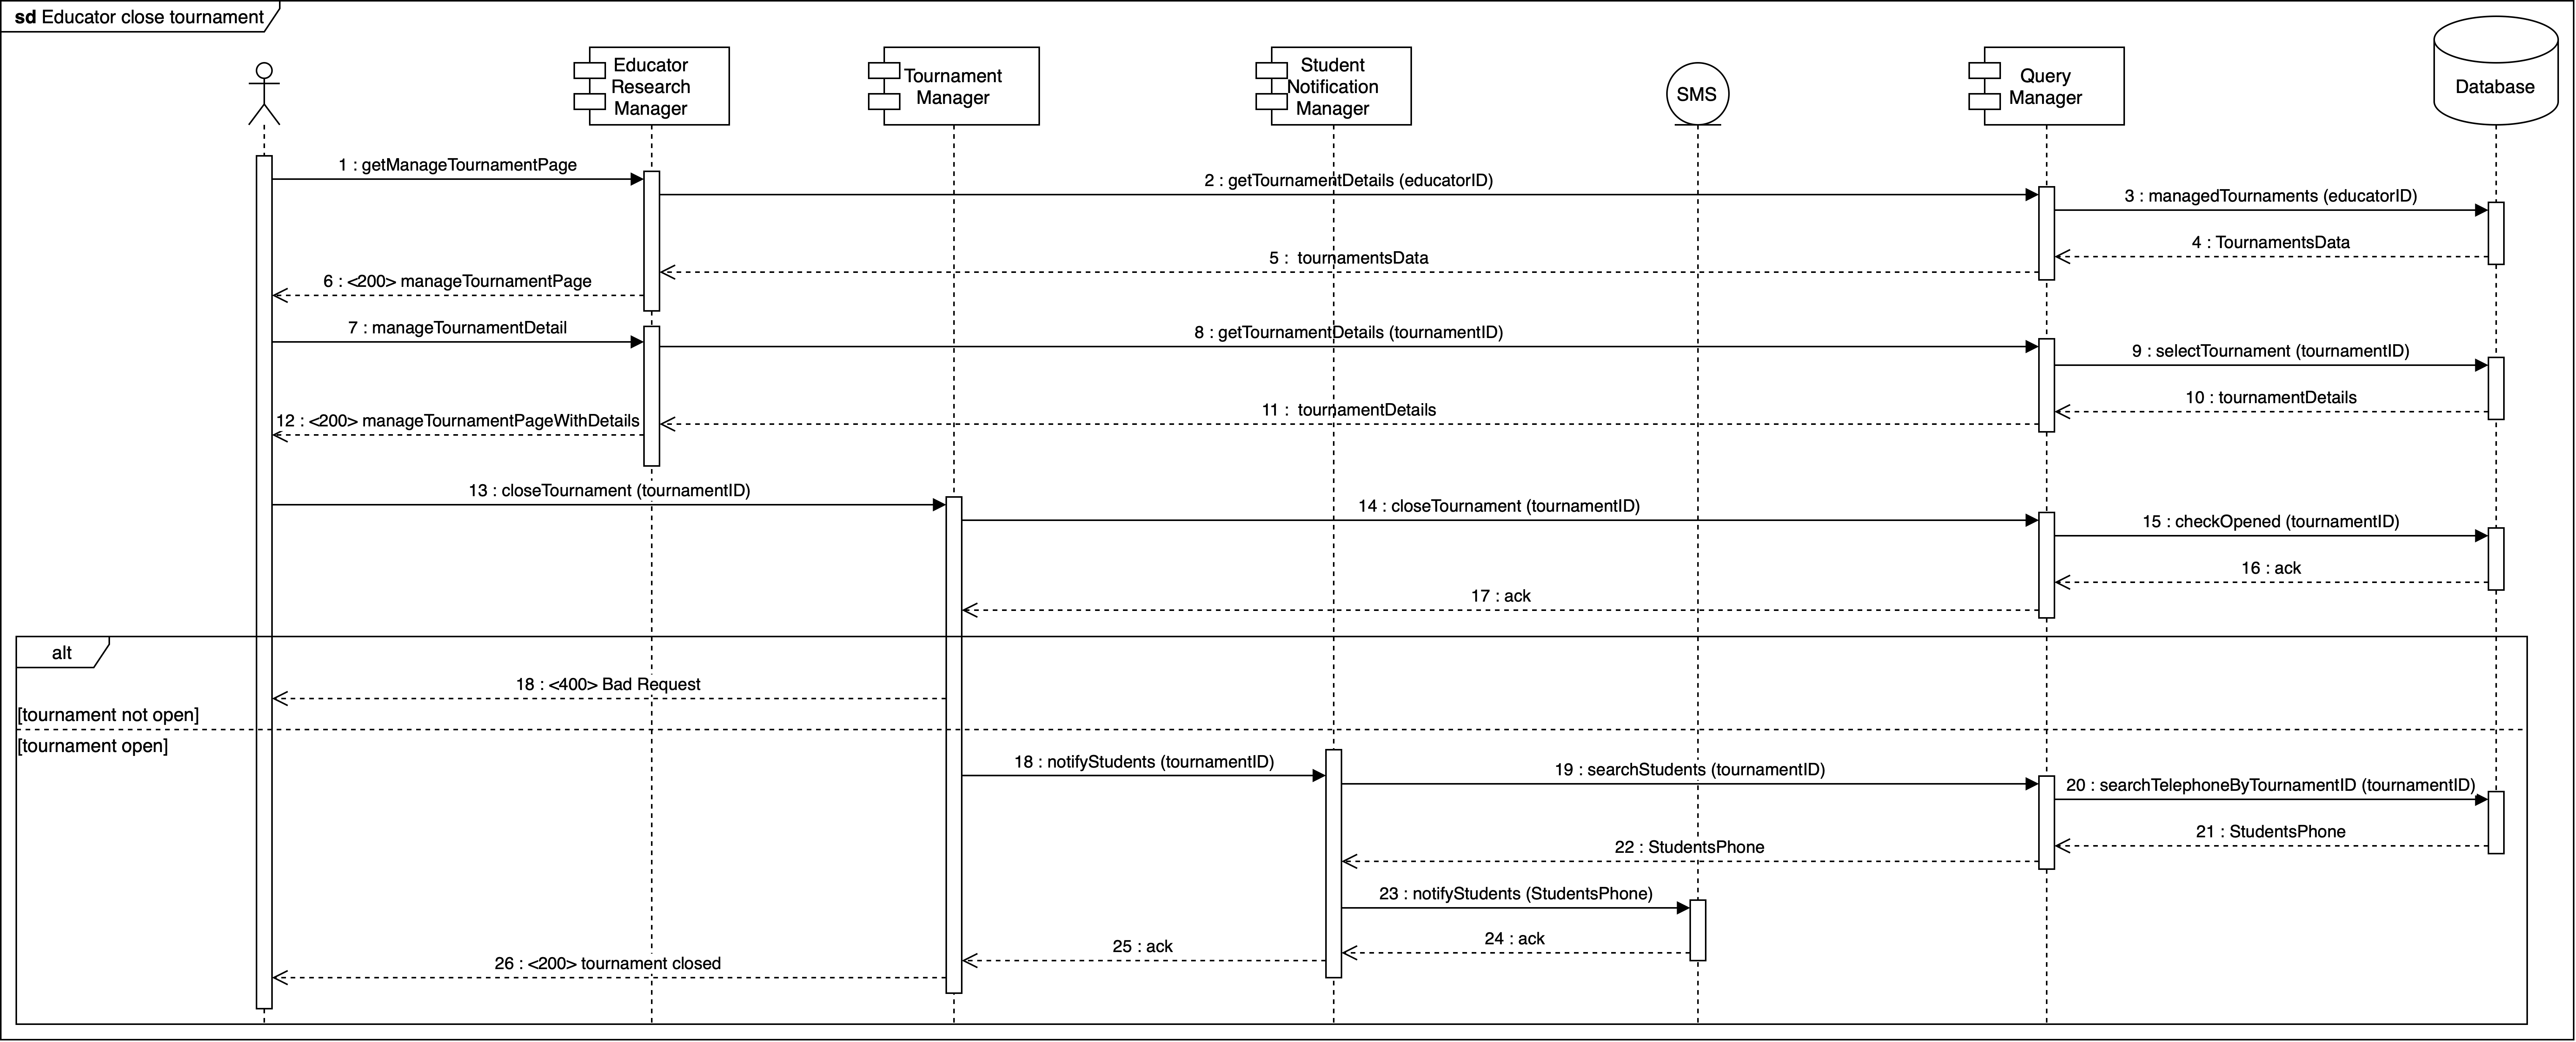
\includegraphics[width=1.0\linewidth]{images/ectrv1.png}
    \end{figure}

    \paragraph*{Educator personal evaluation}
    In this case the actor is an educator that wants to add the personal evaluation to a managed tournament. 
    After accessing the manage battle page and selecting the desired battle he can finally fill out the form with the evaluations.
    If all submitted values are correct the system insert these into the database and notifies the user with a message.
    \begin{figure}[H]
        \centering
        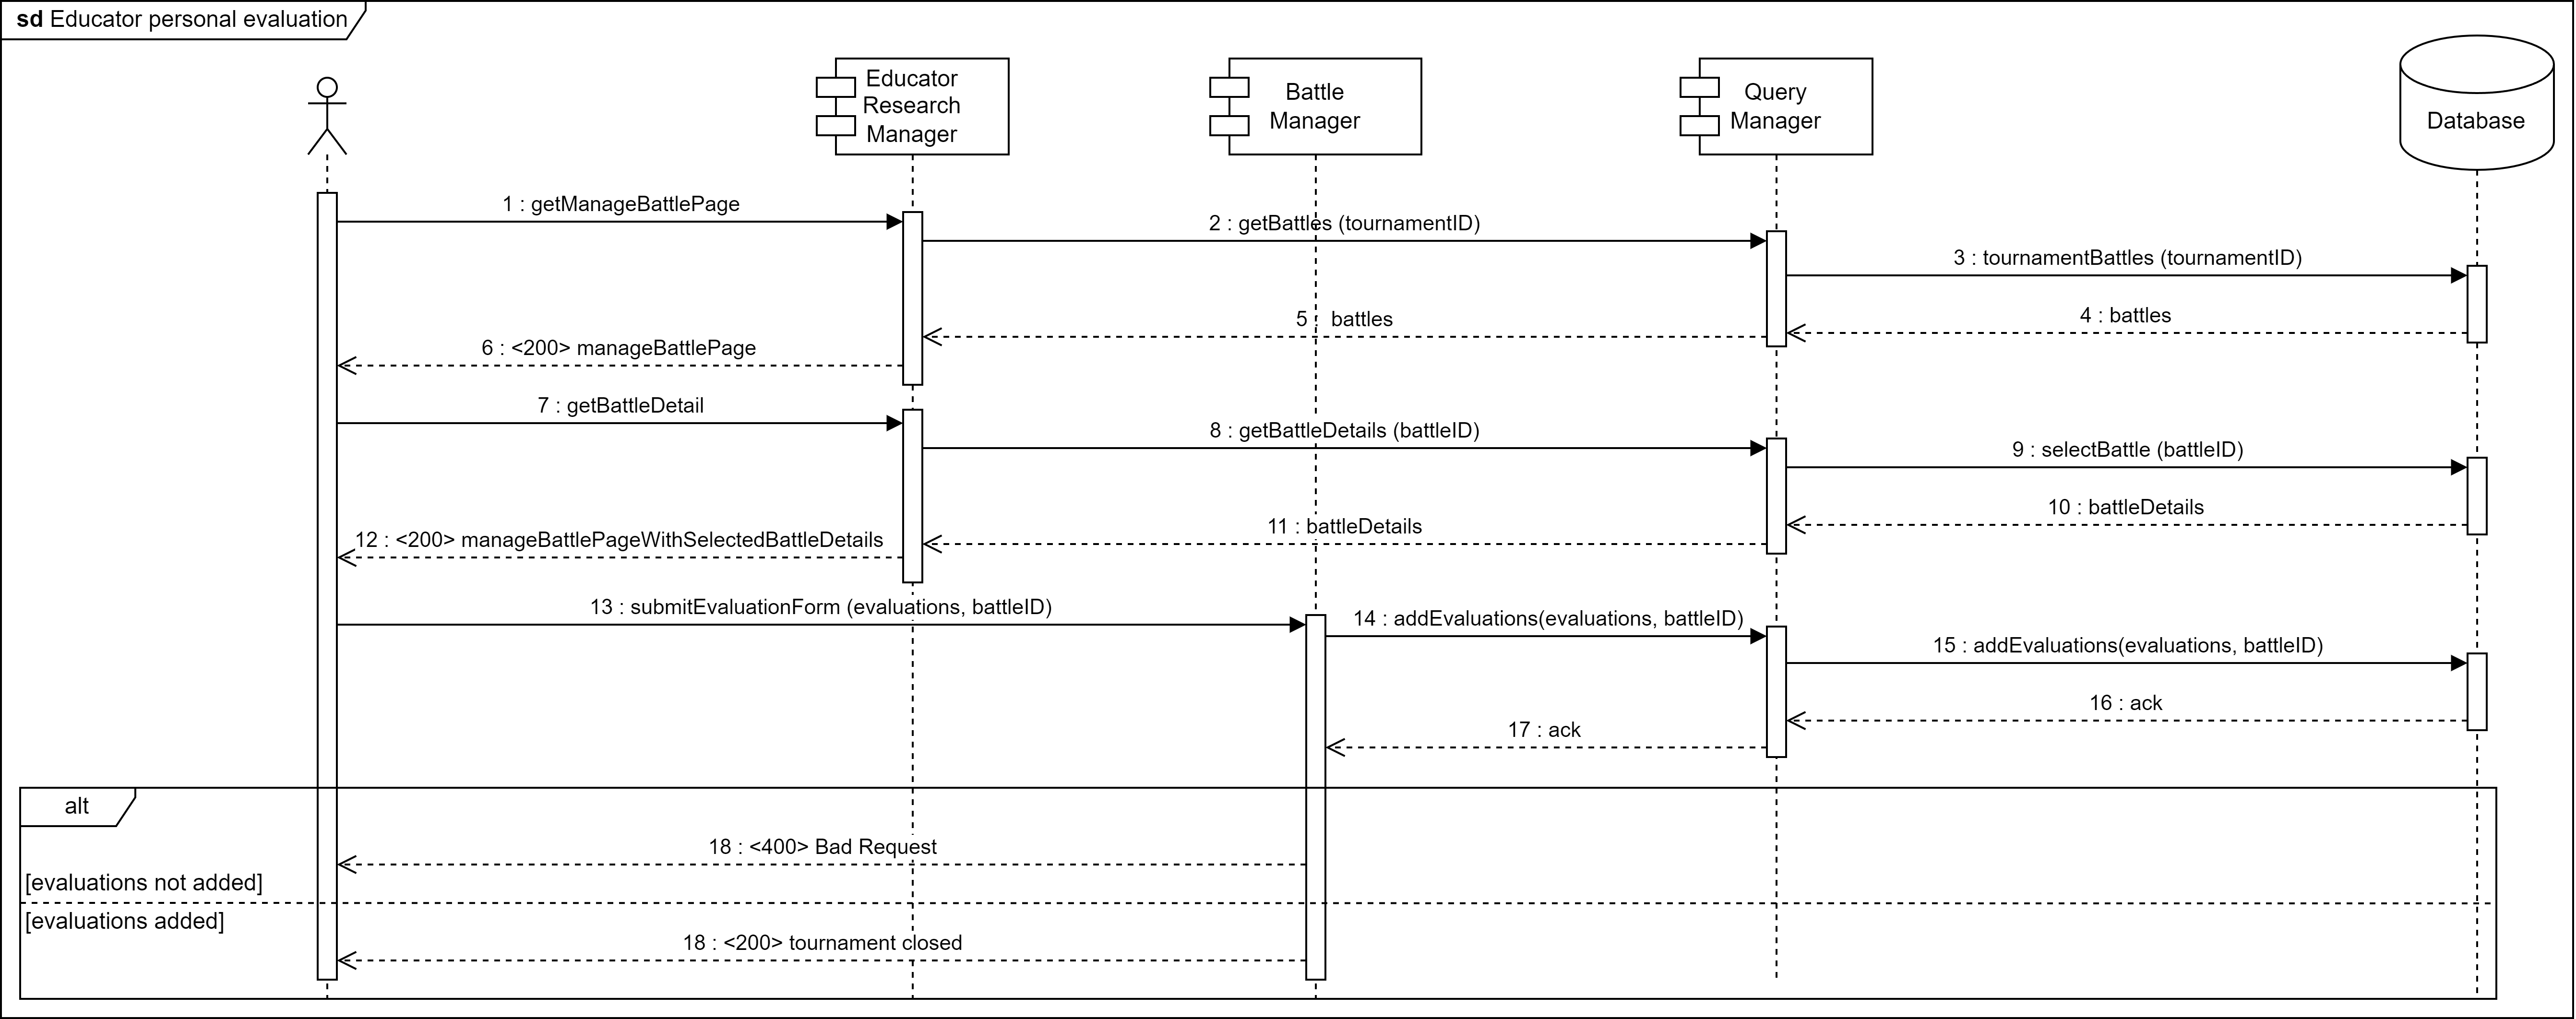
\includegraphics[width=1.0\linewidth]{images/eperv.png}
    \end{figure}

    \paragraph*{User checks tournament leaderboard}
    In this case the user is a registered student that wants to check the leaderboard of a tournament. 
    After accessing the search page and consequently the tournament details page the student can access the leaderboard page of the selected tournament. 
    \begin{figure}[H]
        \centering
        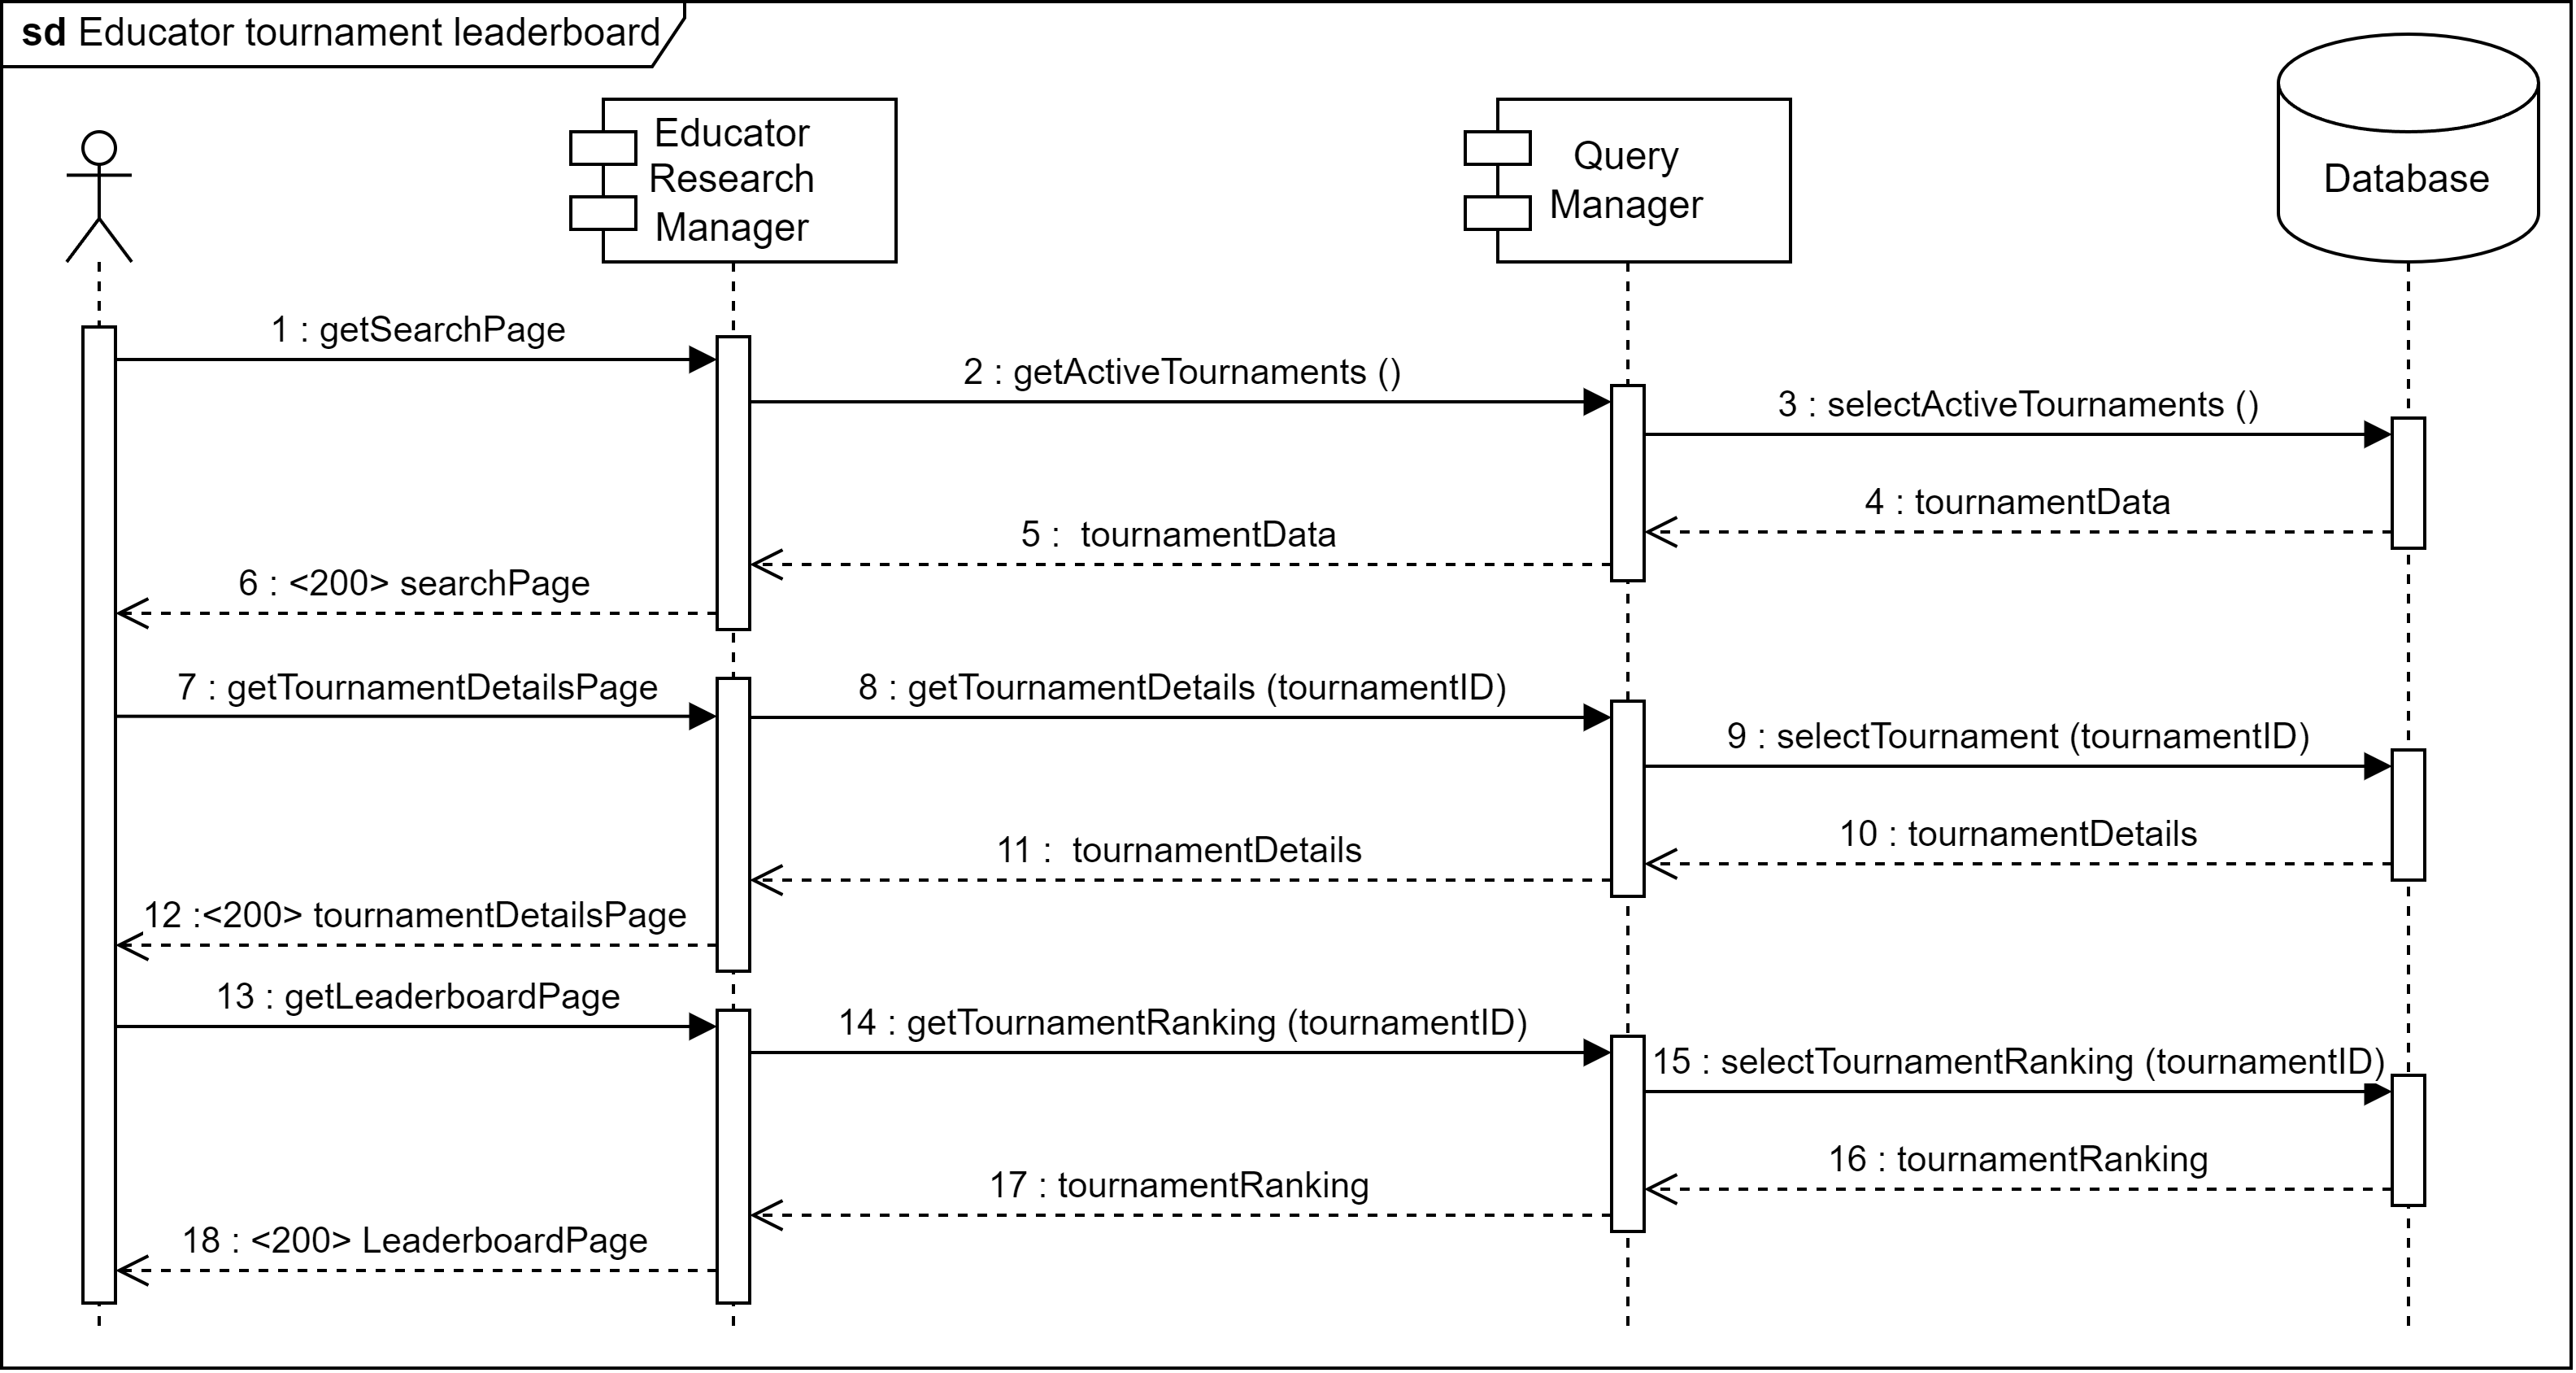
\includegraphics[width=1.0\linewidth]{images/etlrv.png}
    \end{figure}

    \paragraph*{User checks battle leaderboard}
    In this case the user is a registered student that wants to check the leaderboard of a tournament. 
    After accessing the search page and consequently the tournament details page the student can access the leaderboard page of the selected tournament. 
    After this he can click on the button linked to the desired battle within the selected tournament. 
    \begin{figure}[H]
        \centering
        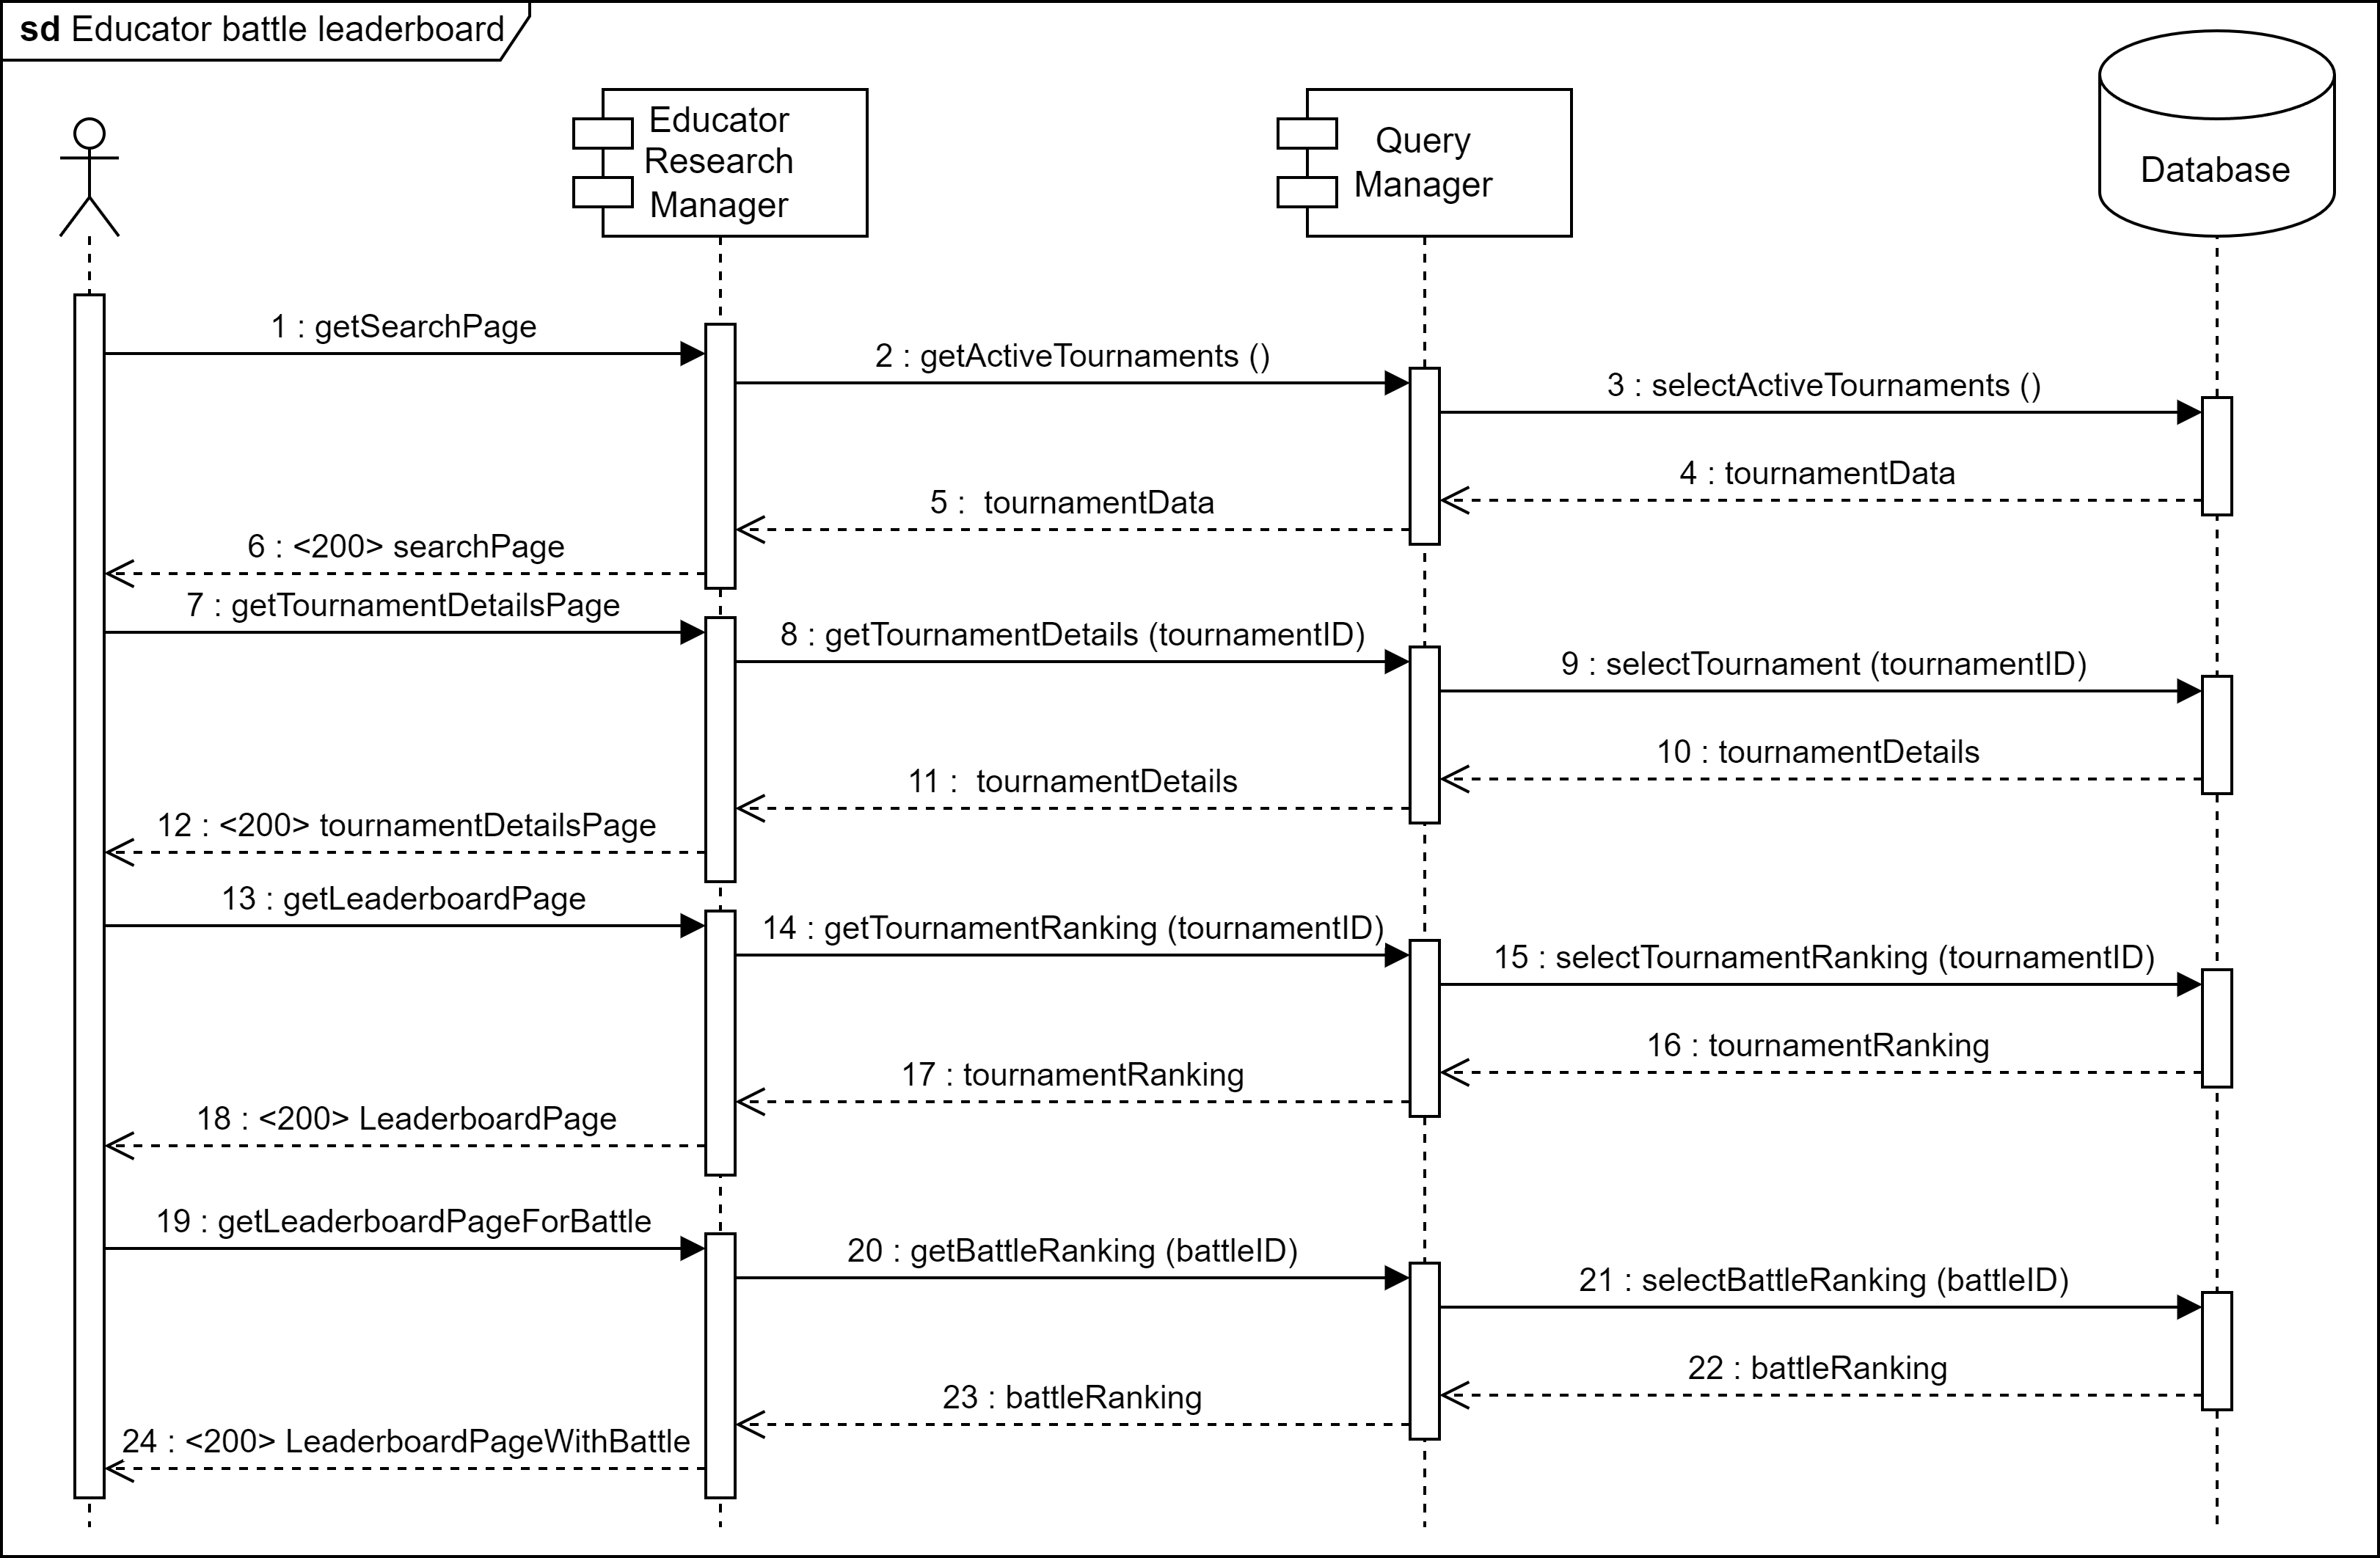
\includegraphics[width=1.0\linewidth]{images/eblrv.png}
    \end{figure}

    \subsection{Automatic runtime view}
    In this section we analyze the runtime views for the automatic evaluation and the closure of a battle. 

    \paragraph*{Automatic evaluation}
    In this case an actor does a commit and the GitHub API notifies the system. 
    The system checks if the battle is still active and in this case it performs the evaluation. 
    After the point computation it assigns the new points to the corresponding group. 
    \begin{figure}[H]
        \centering
        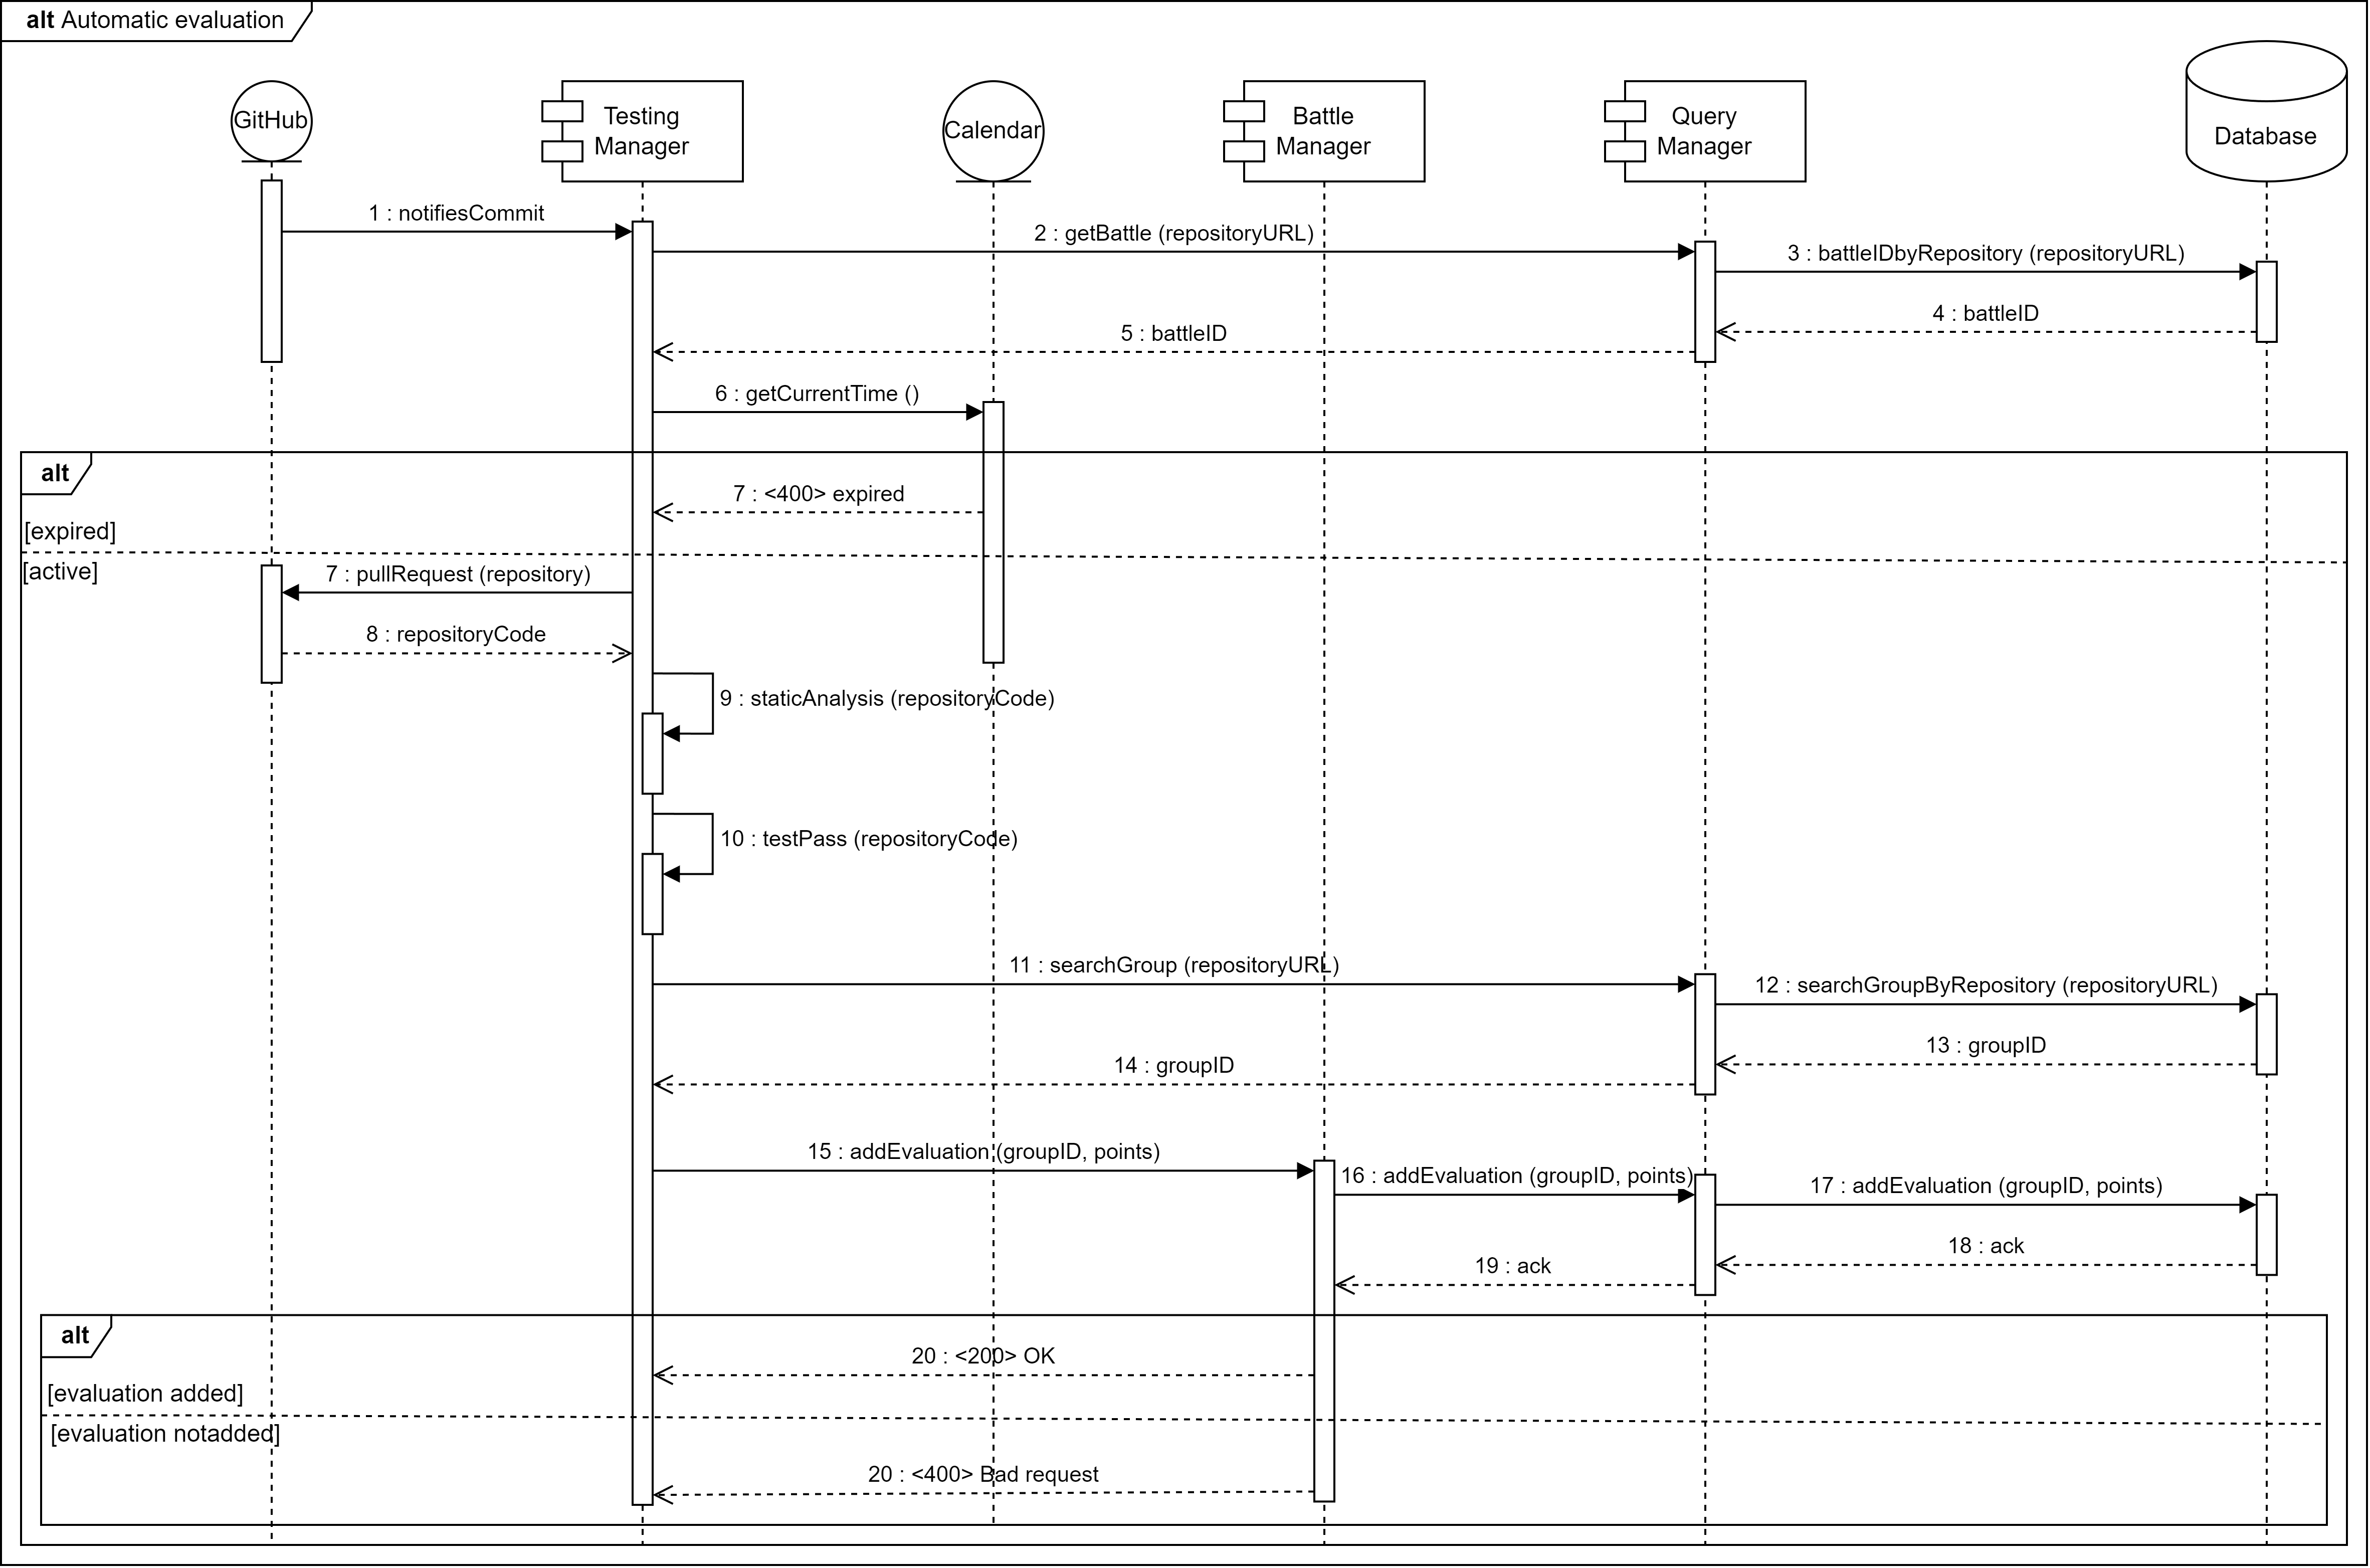
\includegraphics[width=1.0\linewidth]{images/aerv.png}
    \end{figure}

    \paragraph*{Automatic battle closure}
    In this case the calendar API notifies the system about the deadline of a battle.
    The system waits for the personal evaluation if needed. 
    Subsequently, it gives the points to the single students for the tournament ranking and closes the battle. 
    \begin{figure}[H]
        \centering
        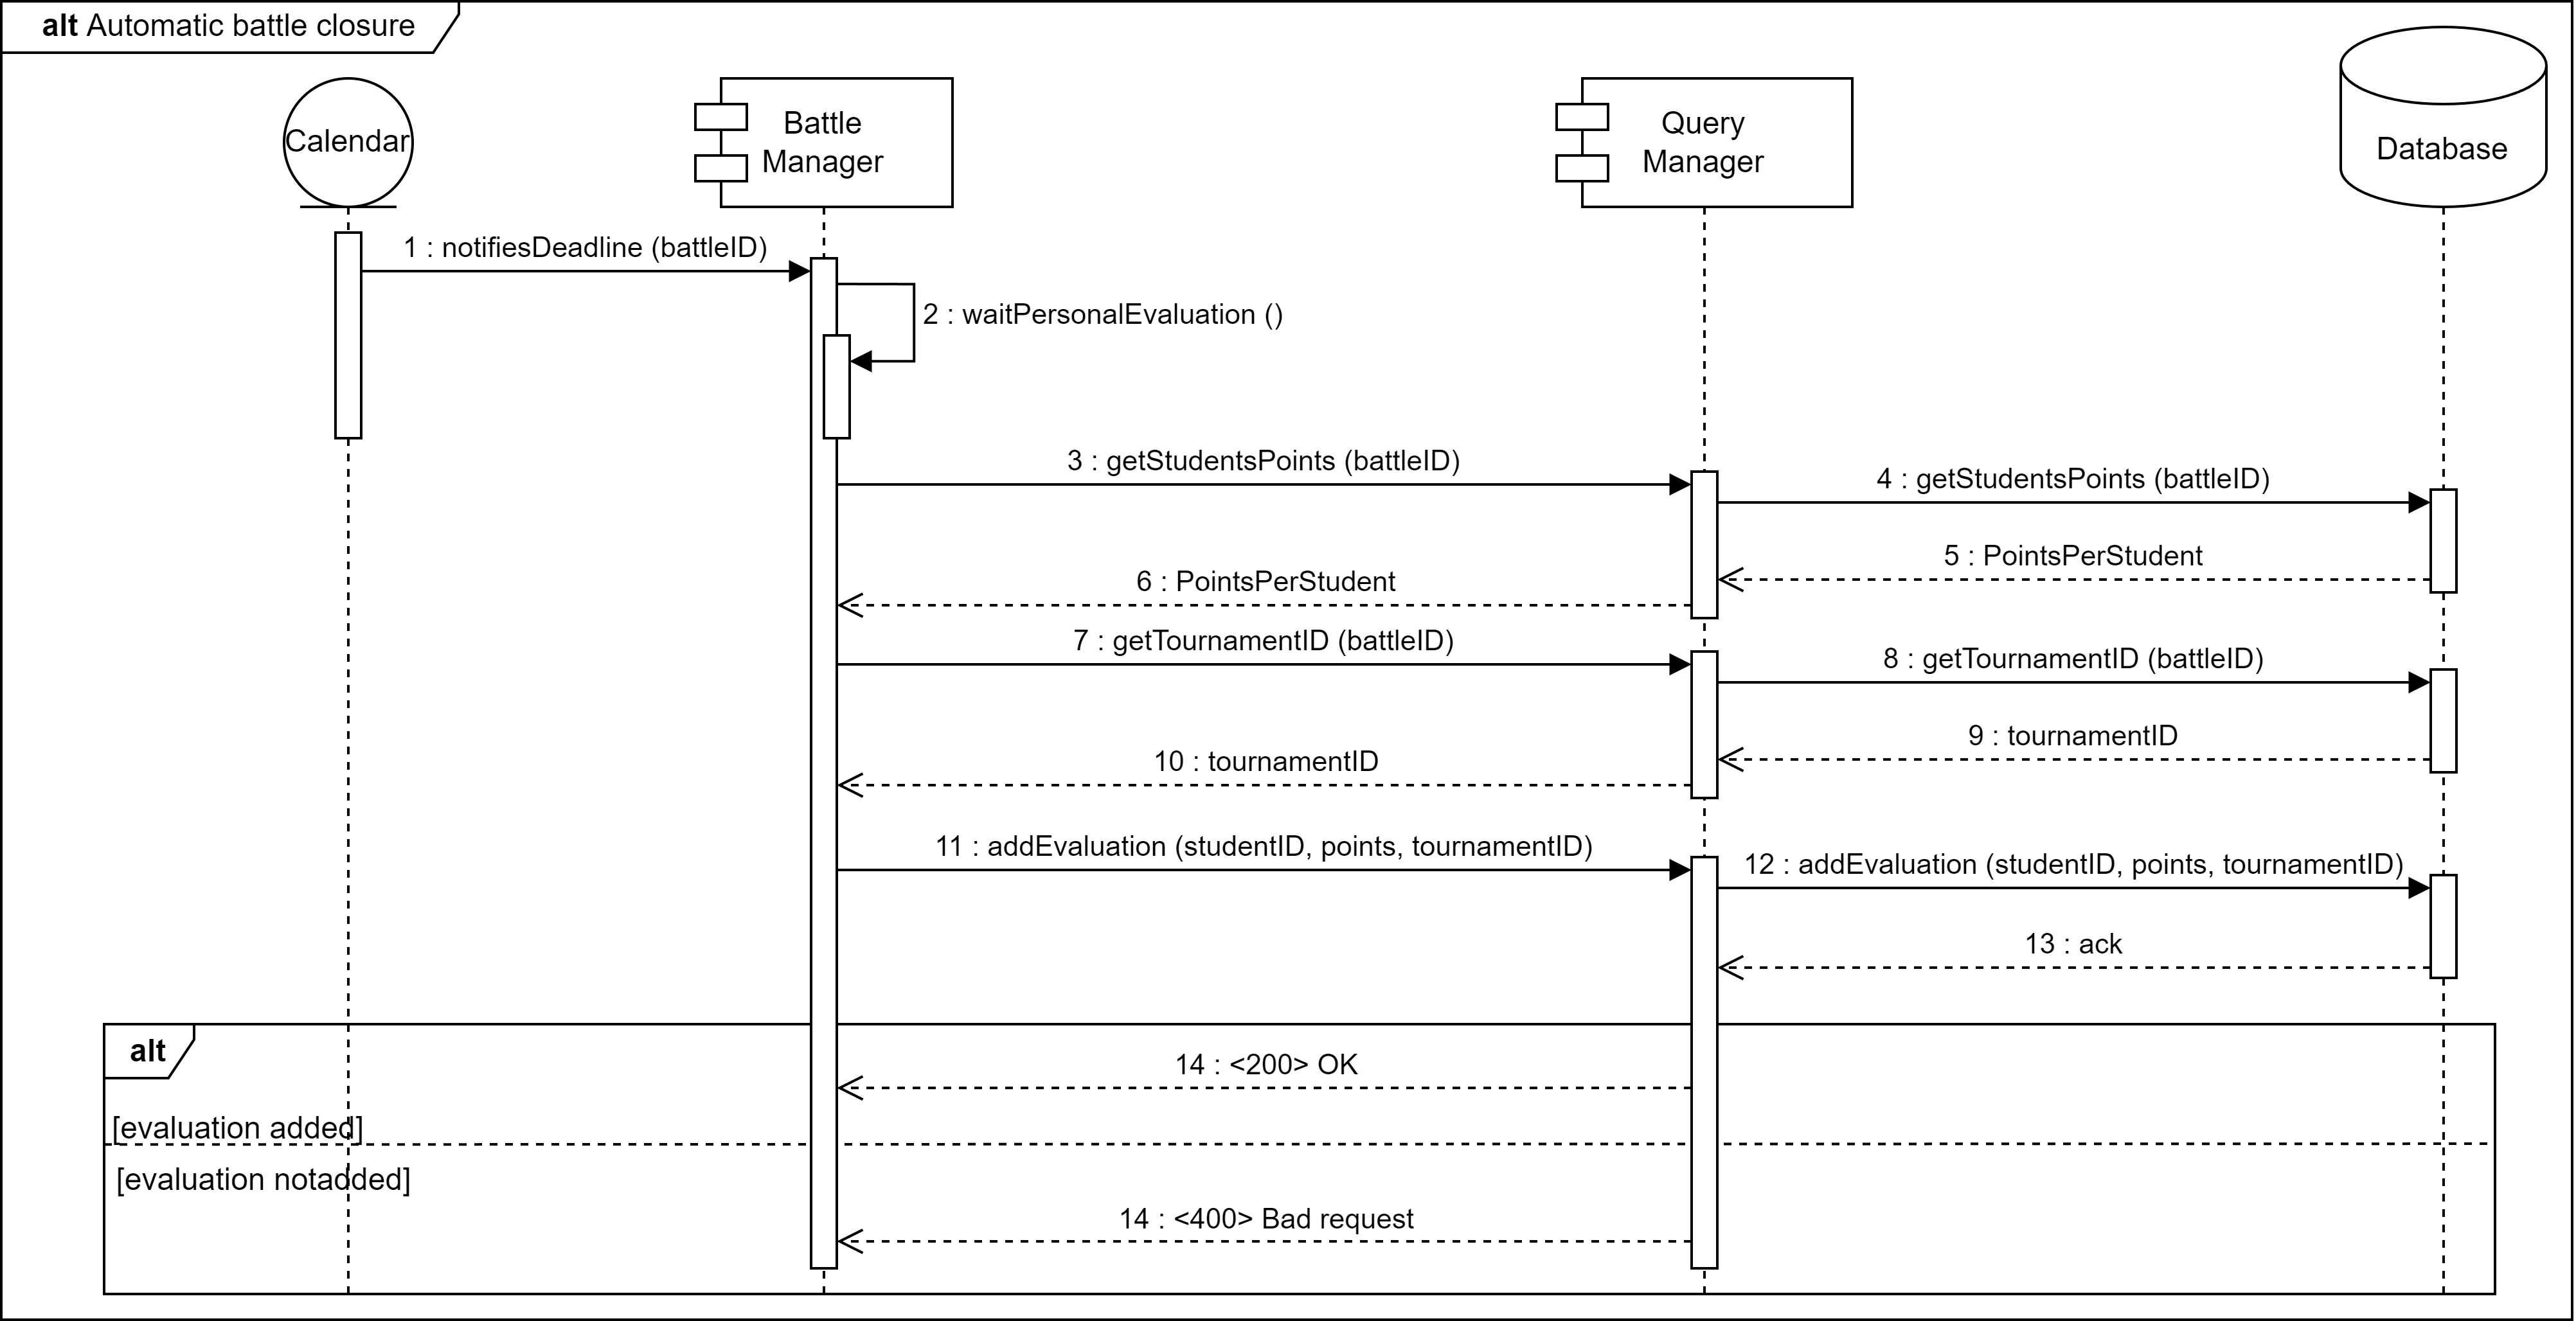
\includegraphics[width=1.0\linewidth]{images/abcrv.png}
    \end{figure}

    \section{Component interfaces}
    All components described in the previous sections utilizes some interfaces to interact with each other. 
    In the following we list all useful interfaces to implemented by considering each component separately. 

    \subsection{Student manager components}
    The student manager employs five components to enable students to access all functionalities. 
    These components will be examined in detail below.

    \paragraph*{Student account manager}
    This component comprises the following interfaces: 
    \begin{itemize}
        \item checkForm(data): checks if all the information submitted by the student are consistent. 
        \item checkUnivoque(username, email, telephone): checks if all these variables are not already in the database. 
        \item createStudent(username, email, telephone, password): create a new student upon verification of the fields. 
        \item createStudentVerificationCode(email, code): add a temporary verification code to the database linked to an email to be verified. 
        \item sendEmail(): send the email with the verification code to the email inserted by the student. 
        \item checkVerificationCode(email, code): checks if the combination of email and code is in the database. 
        \item checkStudentCredentials(email, password): checks if the email and password inserted are in the database. 
        \item createStudentToken(studentID, token): add a new log in token linked to a student. 
    \end{itemize}

    \paragraph*{Tournament subscription manager}
    This component comprises the following interfaces: 
    \begin{itemize}
        \item checkTournament(userID, tournamentID): send a request to the query manager to enroll the student in the given tournament. 
        \item searchTournament (keyword): returns a list of tournaments matching the searched keyword. 
    \end{itemize}

    \paragraph*{Battle subscription manager}
    This component comprises the following interfaces: 
    \begin{itemize}
        \item joinBattle(studentID, battleID): let a student join a certain battle specified by the battleID.
    \end{itemize}

    \paragraph*{Student profile manager}
    This component comprises the following interfaces: 
    \begin{itemize}
        \item getStudentData(username): returns all the information linked to a certain student specified by the username. 
        \item getEnrolledTournament(studentID): returns all the tournaments in which the student is enrolled. 
    \end{itemize}

    \paragraph*{Student research manager}
    This component comprises the following interfaces: 
    \begin{itemize}
        \item getTournaments(): returns a list of active tournament that the student can join. 
        \item getTournamentDetails(tournamentID): returns the details of a tournament given its tournamentID. 
        \item getEnrolledTournaments(studentID): return a list of tournaments in which the student is enrolled.
        \item getTournamentRanking(tournamentID): returns a list of students organized by number of points earned. 
        \item getBattleRanking(battleID): returns a list of groups organized by number of points earned. 
    \end{itemize}

    \paragraph*{Student notification manager}
    This component comprises the following interfaces: 
    \begin{itemize}
        \item searchStudentsPhone(): returns the list of all phone number linked to the students registered in the system. 
        \item notifyStudents(StudentsPhone): notifies all the students with the phone number in the StudentsPhone list. 
        \item searchStudents(tournamentID): searches all student's phone numbers enrolled in the tournament given.
        \item notifyStudents(StudentsPhone, battle): notifies all the students with the phone number in the StudentsPhone list with the identifier of the new battle. 
    \end{itemize}

    \subsection{Educator manager components}
    The educator manager employs five components to enable educators to access all functionalities. 
    These components will be examined in detail below.
    
    \paragraph*{Educator account manager}
    This component comprises the following interfaces: 
    \begin{itemize}
        \item checkForm(data): checks if all the information submitted by the educator are consistent. 
        \item checkUnivoque(username, email, telephone): checks if all these variables are not already in the database. 
        \item createEducator(username, email, telephone, password): create a new educator upon verification of the fields. 
        \item createEducatorVerificationCode(email, code): add a temporary verification code to the database linked to an email to be verified. 
        \item sendEmail(): send the email with the verification code to the email inserted by the educator. 
        \item checkVerificationCode(email, code): checks if the combination of email and code is in the database. 
        \item checkEducatorCredentials(email, password): checks if the email and password inserted are in the database. 
        \item createEducatorToken(educatorID, token): add a new log in token linked to an educator. 
    \end{itemize}

    \paragraph*{Tournament manager}
    This component comprises the following interfaces: 
    \begin{itemize}
        \item getActiveTournaments(): returns a list of all active tournaments. 
        \item searchTournament(keyword): search a tournament which contains the keyword in the name or description. 
        \item createTournament(data): creates a new tournament with the submitted information. 
        \item notifyStudent(): notifies the students.
        \item notifyStudent(tournamentID): notifies the students that are enrolled about the closure of the tournament.
        \item inviteCollaborator(email): invite a new collaborator to manage the tournament. 
        \item closeTournament(tournamentID): closes a tournament with the given tournamentID. 
    \end{itemize}

    \paragraph*{Battle manager}
    This component comprises the following interfaces: 
    \begin{itemize}
        \item createRepository(): creates a new repository and return the URL. 
        \item createBattle(data): creates a new battle within a managed tournament. 
        \item notifyStudents(tournamentID, battleID): notifies all students that are enrolled in the tournament in which the new battle is created. 
        \item addEvaluations(evaluations, battleID): adds the evaluations for each group in a certain battle. 
        \item addEvaluation(groupID, points): adds the points to the group specified. 
        \item waitPersonalEvaluation(): returns true if the evaluation is added or not necessary. 
        \item getStudentsPoints(battleID): returns the points given to each student in a given battle. 
        \item getTournamentID(battleID): returns the tournamentID where the battle was created. 
        \item addEvaluation(studentID, points, tournamentID): updates the points linked to the tournament leaderboard. 
    \end{itemize}

    \paragraph*{Educator profile manager}
    This component comprises the following interfaces: 
    \begin{itemize}
        \item getEducatorData(username): returns all the information linked to a certain educator specified by the username. 
        \item getEnrolledTournament(educatorID): returns all the tournaments in which the educator is enrolled. 
    \end{itemize}

    \paragraph*{Educator research manager}
    This component comprises the following interfaces: 
    \begin{itemize}
        \item getTournaments(): returns a list of active tournament that the educator can view. 
        \item getTournamentDetails(eduatorID): returns a list of tournament managed by the educator with the given educatorID. 
        \item getTournamentDetails(tournamentID): returns all the details of the given tournament. 
        \item getBattles(tournamentID): returns all battles within a given tournament. 
        \item getBattleDetails(battleID): returns all the details of the given battle. 
        \item getActiveTournaments(): returns a list of all active tournaments.
        \item getTournamentRanking(tournamentID): returns a list of students organized by number of points earned. 
        \item getBattleRanking(battleID): returns a list of groups organized by number of points earned. 
    \end{itemize}

    \paragraph*{Testing manager}
    This component comprises the following interfaces: 
    \begin{itemize}
        \item getBattle(repositoryURL): return the ID of the battle related to the give repository. 
        \item getCurrentTime(): return the current time to check if a battle is active or not. 
        \item staticAnalysis(repositoryCode): performs the static analysis and returns a certain amount of points. 
        \item testPass(repositoryCode): computes how many test cases are passed and returns a certain amount of points. 
        \item searchGroup(repositoryURL): returns the groupID related to the give repository URL. 
        \item addEvaluation(groupID, points): adds the points to the group specified. 
        \item notifiesCommit(repositoryUrl): is called by GitHub, through an automated workflow, in order to trigger the CKB platform,
              pull the latest committed code and evaluate it. 
        \end{itemize}

    \subsection{Query manager}
    The schema of the database is described in the component view section. 
    The system interacts with these tables with the following interfaces: 
    \begin{itemize}
        \item selectStudent(username): search a student with a certain username. 
        \item insertStudent(query): add a student with query data (username, email, telephone, and password).
        \item insertStudentVerificationCode(query): add a verification code to a certain student with query data (studentID and code). 
        \item selectVerificationcode(query): search the student through the studentID and the code; if they match the code is correct. 
        \item selectStudent(email, password): search a student with the combination of email and password given. 
        \item insertStudentToken(studentID, token): associate a student with a certain token used to maintain the session active client side. 
        \item selectEnrolledTournament(studentID): returns all the tournaments where the student is enrolled. 
        \item selectActiveTournaments(): returns all the active tournaments. 
        \item joinTournament(userID, tournamentID): let a student with a certain studentID enroll in a tournament with tournamentID. 
        \item selectTournament(keyword): search all the tournaments with the name or description that matches a given keyword. 
        \item selectTournament(tournamentID): search the tournament with the given tournamentID. 
        \item enrollInBattle(battleID): checks if the student is enrolled in the battle's tournament and if so it enrolls the student in the battle. 
        \item selectTournament (studentID): returns all the tournament in which the student with studentID is enrolled. 
        \item selectTournamentRanking(tournamentID): returns the ranking of the tournament with a certain tournamentID. 
        \item selectBattleRanking(battleID): returns the ranking of a battle in a tournament with a certain battleID. 
        \item selectEducator(username): search an educator with a certain username. 
        \item insertEducator(query): add an educator with query data (username, email, telephone, and password). 
        \item insertEducatorVerificationCode(query): add a verification code to a certain educator with query data (educatorID and code). 
        \item selectEducator(email, password): search an educator with the combination of email and password given. 
        \item insertEducatorToken(educatorID, token): associate an educator with a certain token used to maintain the session active client side. 
        \item selectEducator(username): returns all the data linked with the educator with the given username. 
        \item selectManagedTournament(educatorID): returns all the tournament managed by an educator with a certain educatorID. 
        \item addTournament(data): when the educator submits all the information about a new tournament this interface adds it to the database. 
        \item searchAllStudentsPhone(): returns all the phone numbers in the database regarding the students. 
        \item managedTournaments(educatorID): returns a list of managed tournaments by a given educator. 
        \item addBattle(data): when the educator submits all the information about a new battle this interface adds it to the database. 
        \item searchTelephoneByTournamentID(tournamentID): returns all the telephone numbers of the students enrolled in a given tournament. 
        \item checkExistence(email): checks if the given email is in the educators' table. 
        \item checkOpened(tournamentID): checks the value of the opened attribute for a given tournament. 
        \item selectBattle(battleID): returns all the details of a certain battle. 
        \item addEvaluations(evaluations, battleID): given a list of evaluations and groupID add the personal evaluation in a certain battle for the selected groups. 
        \item battleIDbyRepository(repositoryURL): returns the battleID of the group linked to the repositoryURL. 
        \item searchGroupByRepository(repositoryURL): searches a groupID linked to the repositoryURL given. 
        \item addEvaluation(groupID, points): adds the points to the group specified. 
        \item getStudentsPoints(battleID): returns the points given to each student in a given battle. 
        \item getTournamentID(battleID): returns the tournamentID where the battle was created. 
        \item addEvaluation(studentID, points, tournamentID): updates the points linked to the tournament leaderboard. 
    \end{itemize}

    \section{Selected architectural styles and patterns}
    \begin{itemize}
        \item \textit{Three layers}: the system is divided in three distinct layers, each of them accomplishes a specific task.
            In particular there are the presentation layers, the business logic layer and the data storage layer.
            The use of a three layers architecture makes the system more modular and easier to implement, modify and maintain even between different teams.
            Another advantage is that this modularization allows the use of load balancers between the various servers.
            One last big advantage is that this architecture grants a high data security level, since the data can be accessed only by the application server.
        \item \textit{Adapter Pattern}: in order to retrieve data in a simplified way, a query manager will be implemented.
            The choice of implementing an adapter pattern alloys to keep the application logic independent of the DBMS provider, hiding un necessary and complex parts. 
            The pattern, lastly, also grants a higher level of security since only a preset of operations is available. 
        \item \textit{Separation between Educators and Students}: Educators and Students have completely separated modules, this choice allows for a better modularization,
            enhances the system maintainability and, for future updates, allows to implement features more easily. 
    \end{itemize}

    \section{Other design decisions}
        \subsection{Database choices}
        Previously, an Entity-Relationship (ER) model for the database was introduced, along with a deployment perspective.
        The decision has been made to host the database on a single node.
        This choice stems from the fact that the majority of the data is essential for all users.
        For instance, tournament and battle details are accessible to all users, rendering the utilization of separate databases unnecessary.
        
        \subsection{RESTful APIs}
        We opted for a REST API as the means of communication between backend and frontend.
        This API is built on standard web technologies, facilitating seamless consumption and integration with other systems, such as GitHub.

\chapter{User interface design}
    The user interface is the visual representation of how the application appears to the end user.
    It should be intuitive and straightforward, ensuring easy access to all features.
    Mockups were introduced in the RASD document, and now flowcharts for both students and educators will be presented.
    Flowcharts offer a concise and clear overview of the interactions and steps involved in utilizing the web app.

    \section{Flowchart for students UI}
    \begin{figure}[H]
        \centering
        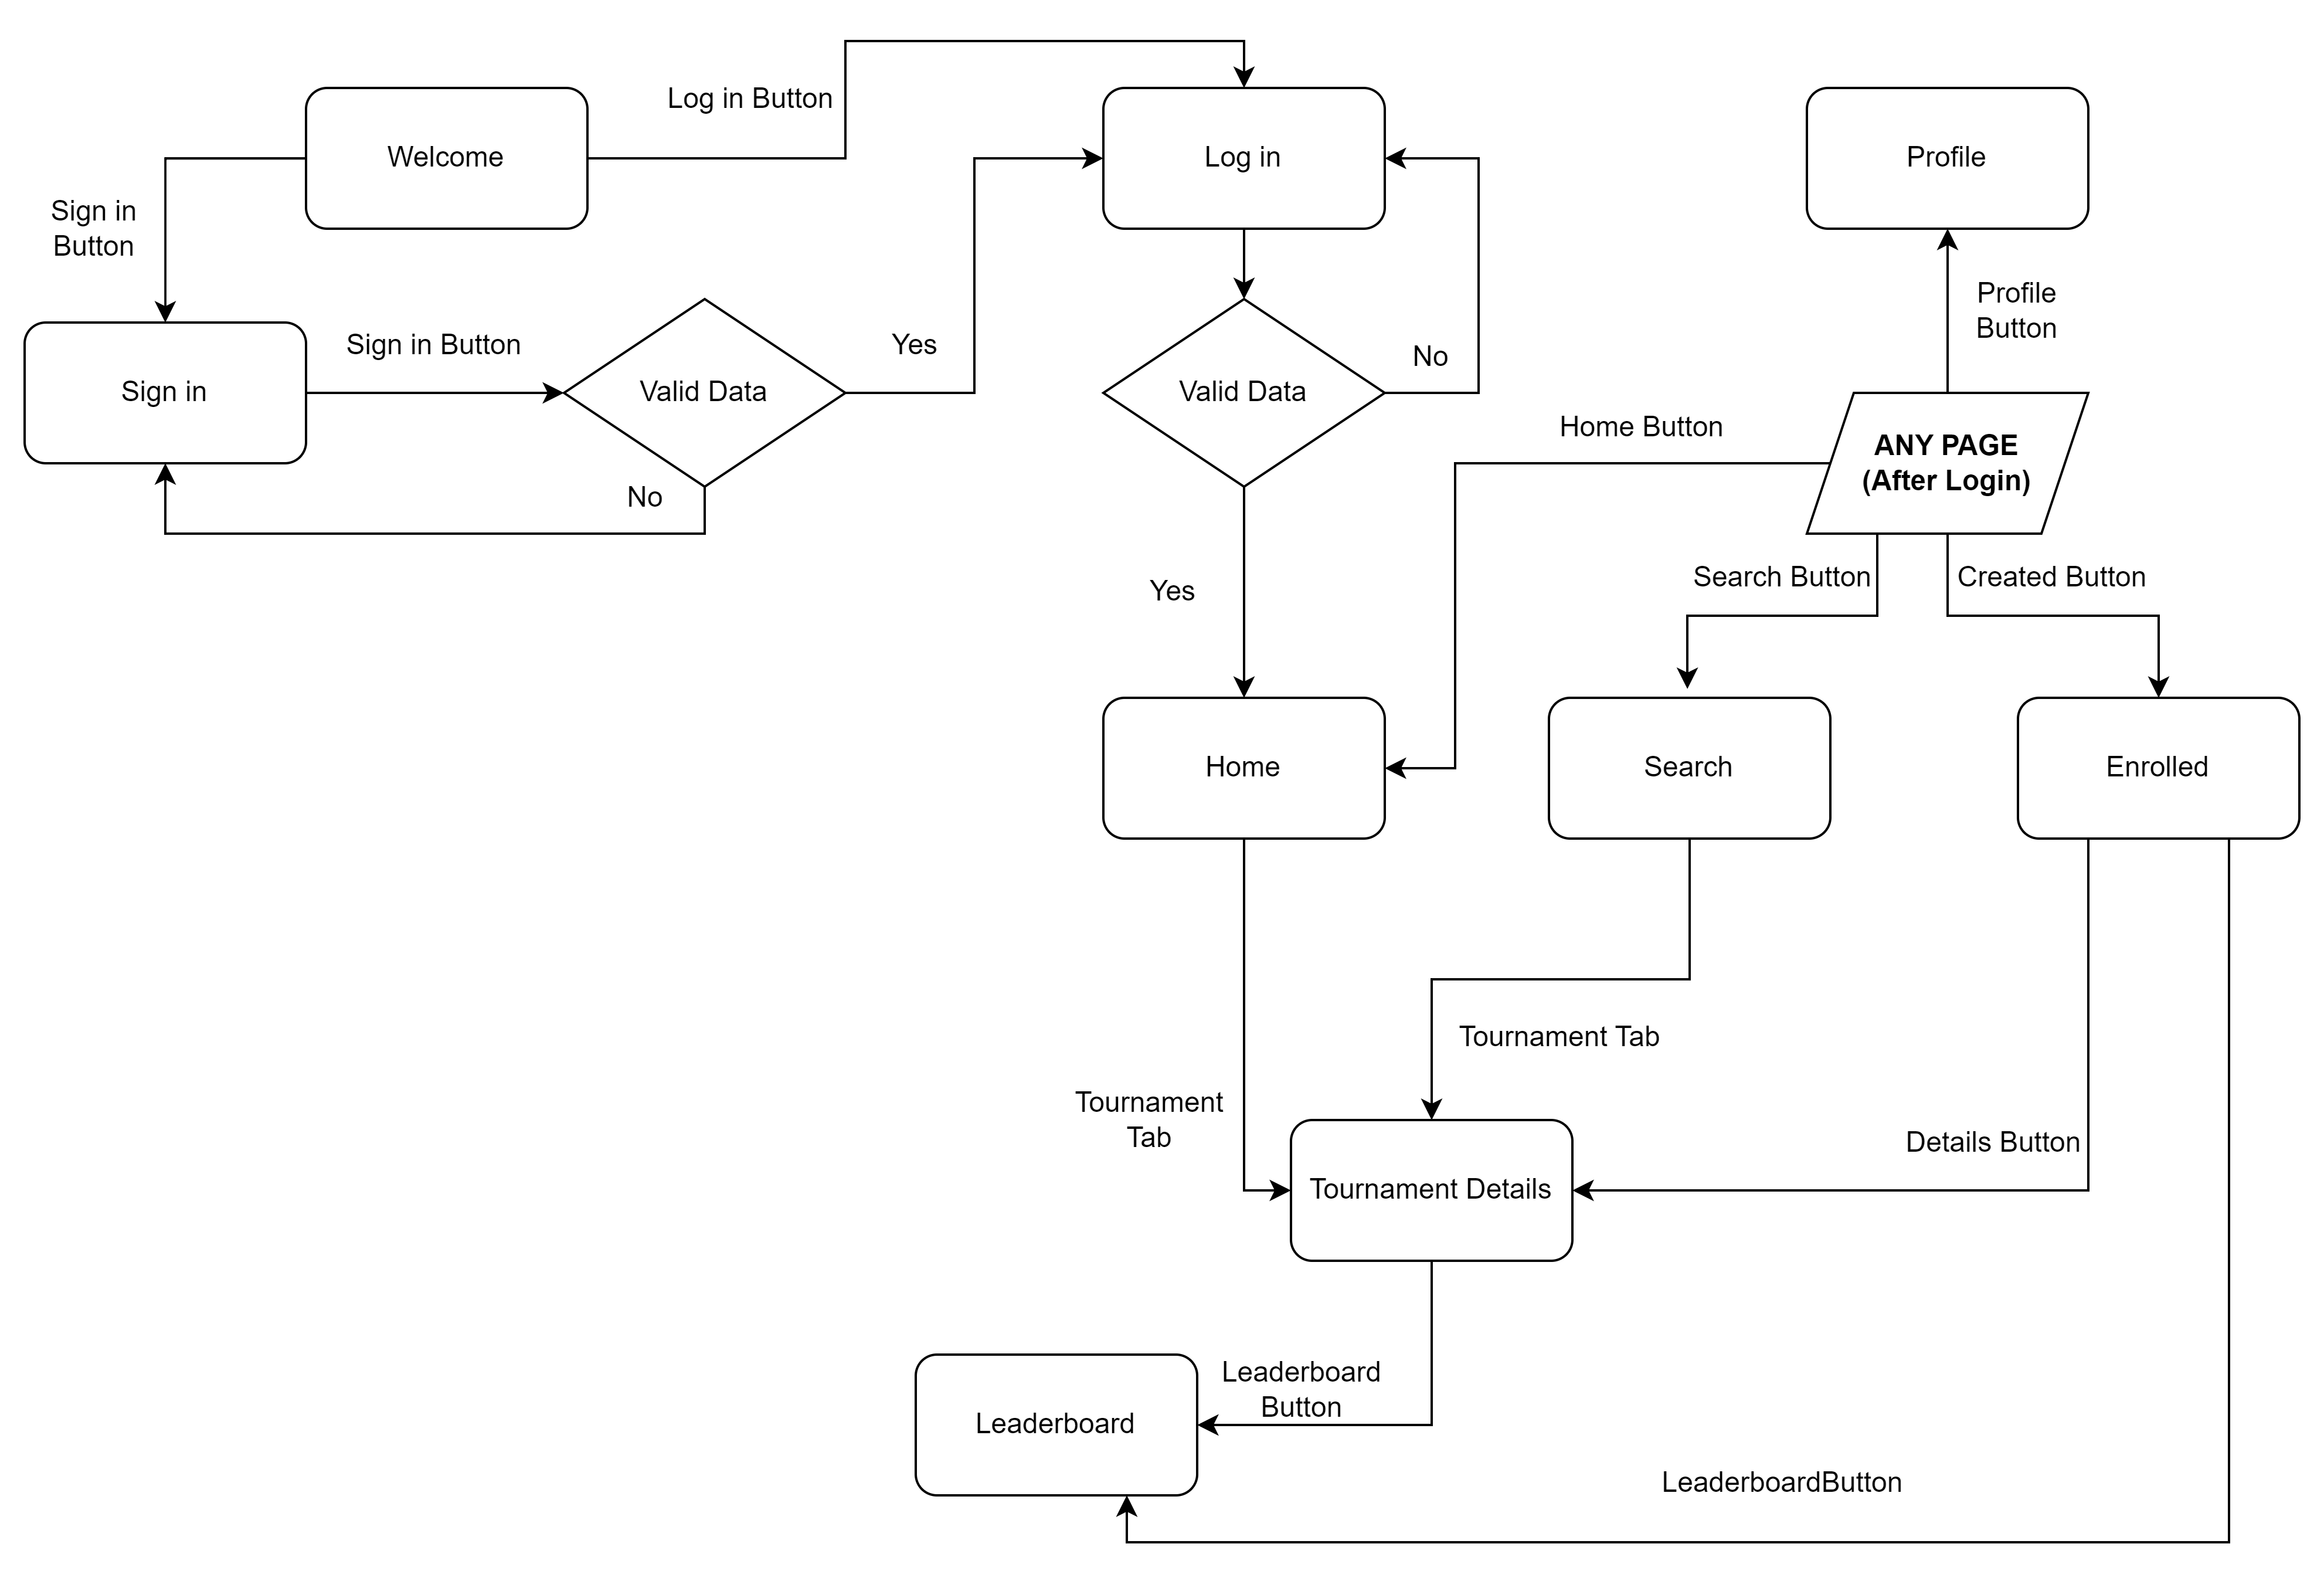
\includegraphics[width=0.9\linewidth]{images/students_UI.png}
    \end{figure}

    \section{Flowchart for educators UI}
    \begin{figure}[H]
        \centering
        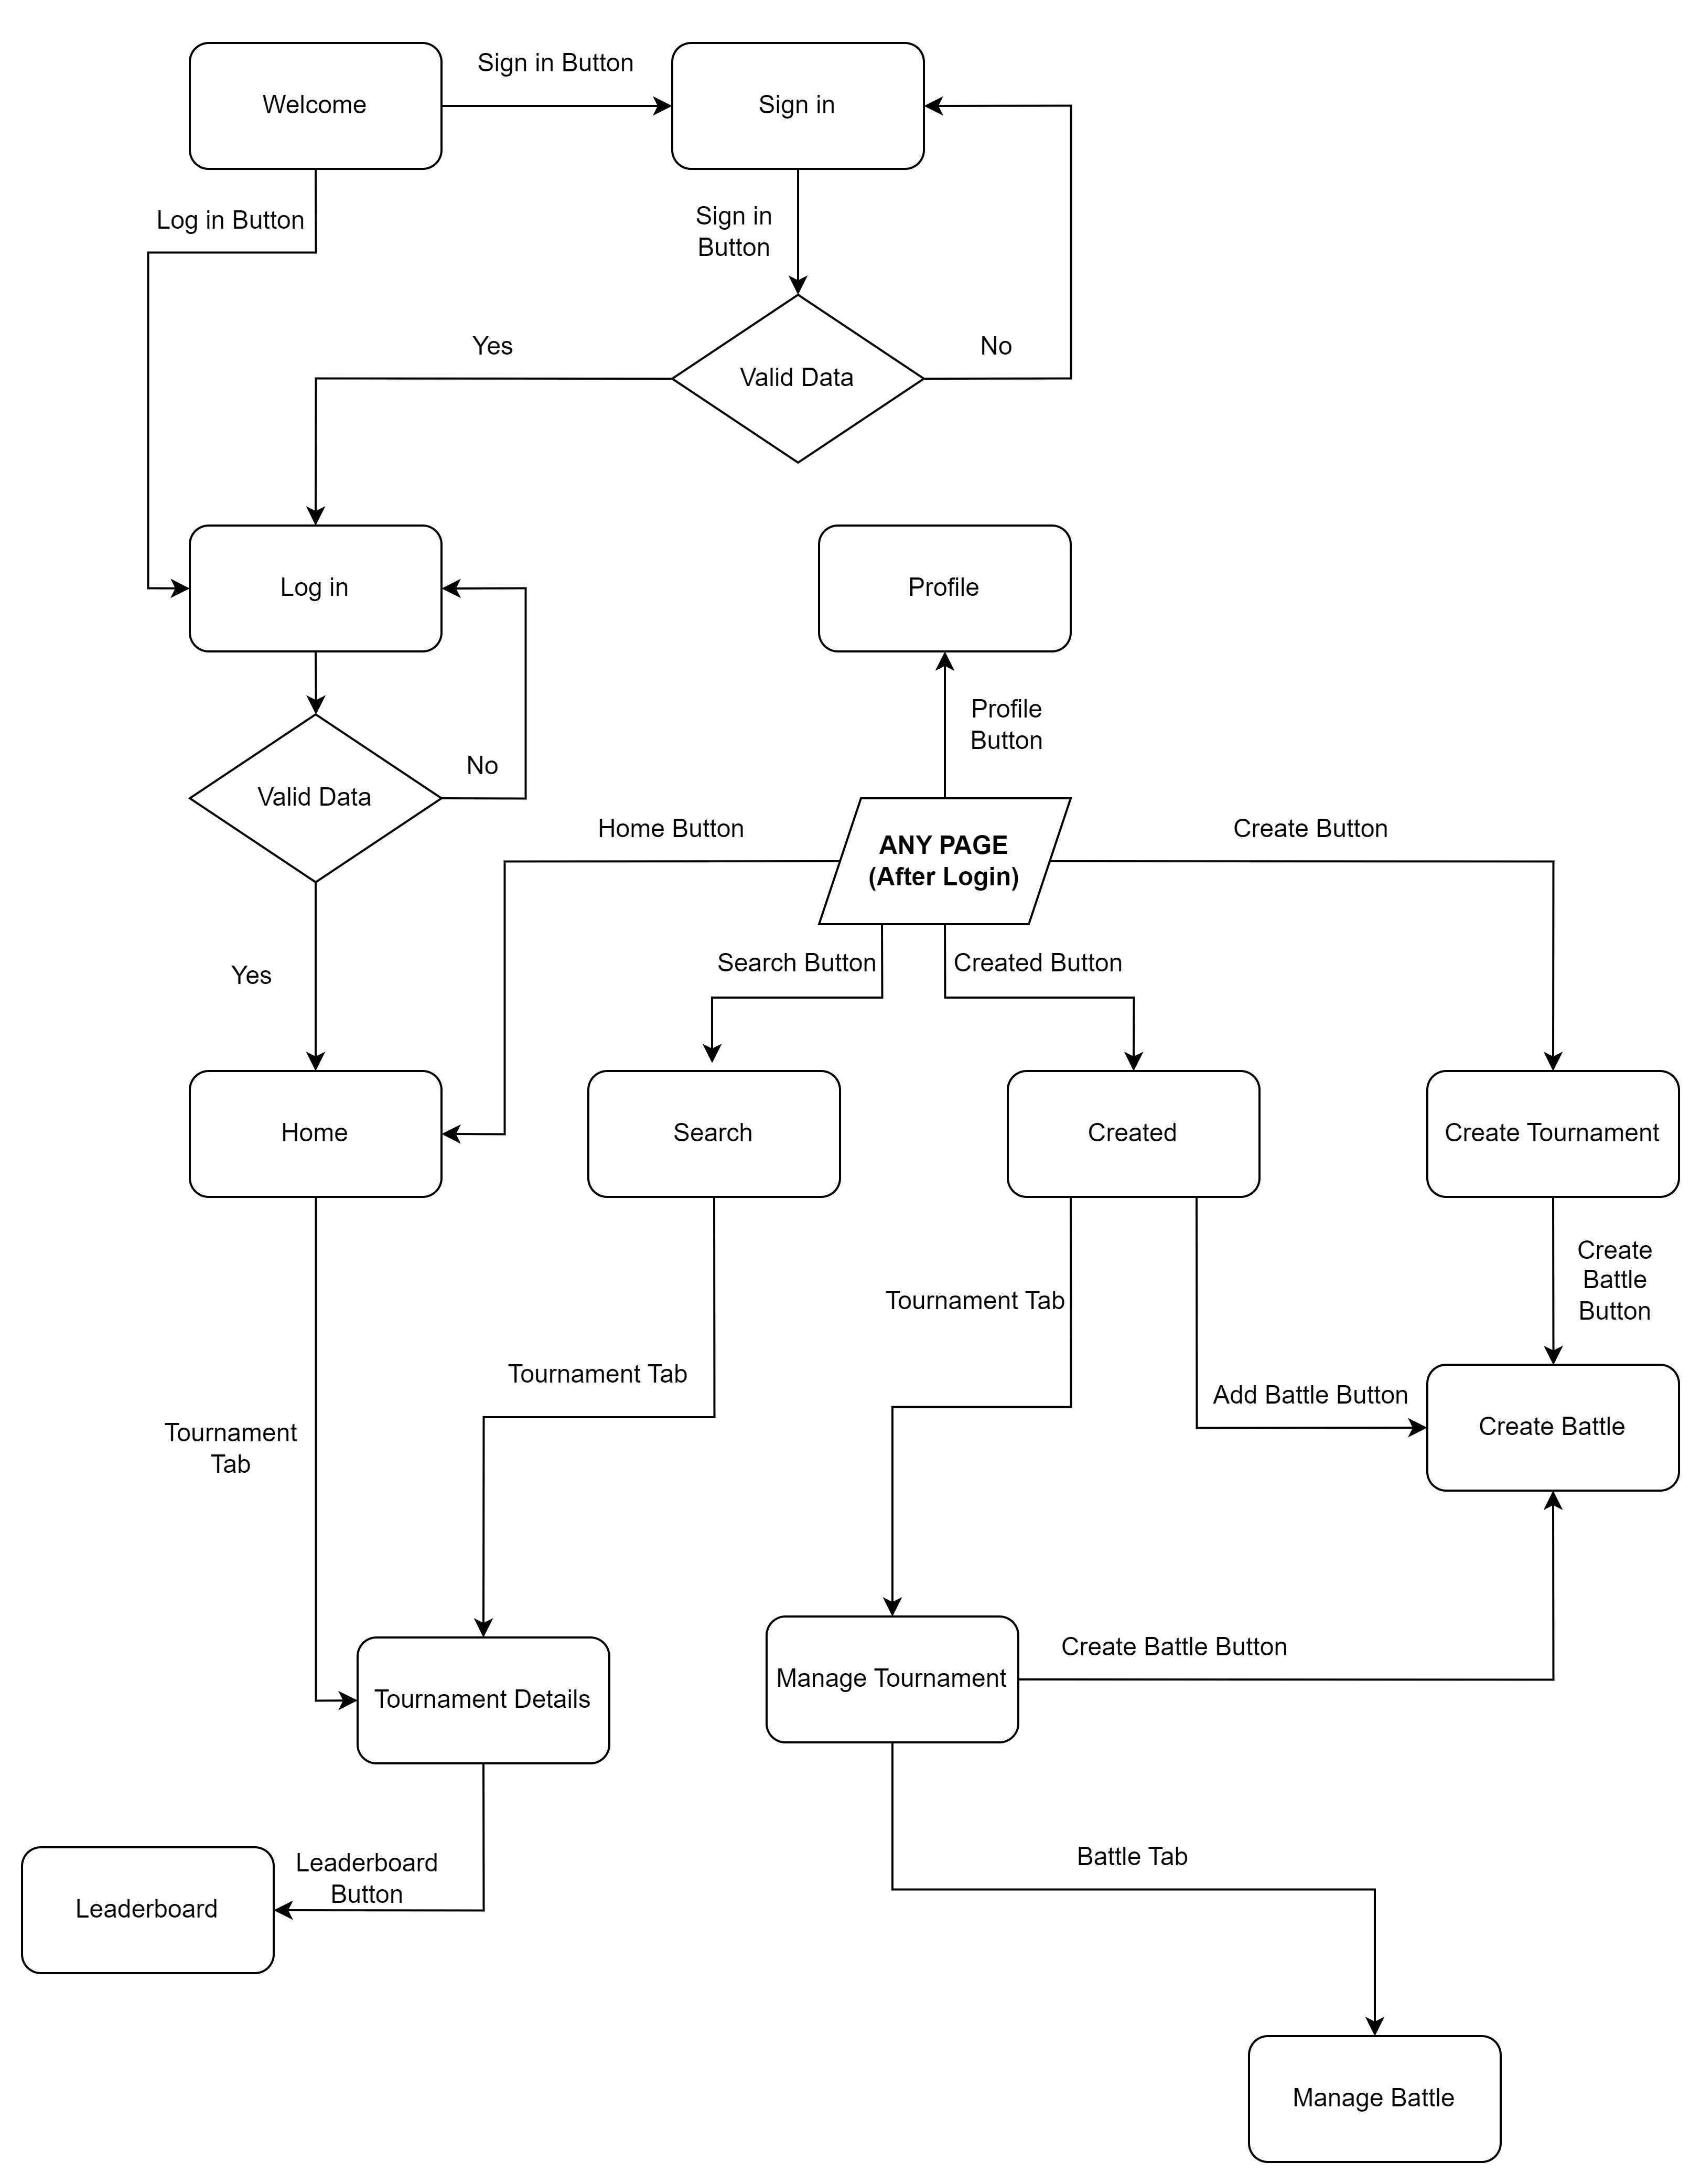
\includegraphics[width=0.9\linewidth]{images/educators_UI.png}
    \end{figure}

\chapter{Requirements traceability}

In the RASD document the requirements of the system to be, needed in order to accomplish the system's purpose,
were presented and in this section those will be mapped to the elements presented in this document.
As the Query Manager is needed for every operation it will be not reported in the mapping below.

\begin{table}[H]
    \begin{tabularx}{\textwidth}{X}
    \textbf{R1} The system allows unregistered students to register.\\
    \hline 
    \textbf{Student Account Manger}
\end{tabularx}
\end{table}


\begin{table}[H]
    \begin{tabularx}{\textwidth}{X}
    \textbf{R2} The system allows registered students to login.\\
    \hline 
    \textbf{Student Account Manger}
\end{tabularx}
\end{table}

\begin{table}[H]
    \begin{tabularx}{\textwidth}{X}
    \textbf{R3} The system allows students to search the tournaments.\\
    \hline 
    \textbf{Student Research Manger, Student Account Manger}
    \end{tabularx}
\end{table}

\begin{table}[H]
    \begin{tabularx}{\textwidth}{X}
    \textbf{R4} The system allows students to enroll in a tournament.\\
    \hline 
    \textbf{Tournament Subscription Manger, Student Account Manger}
    \end{tabularx}
\end{table}

\begin{table}[H]
    \begin{tabularx}{\textwidth}{X}
    \textbf{R5} The system is able to notify students about the creation of a new tournament.\\
    \hline 
    \textbf{Student Notification Manger, Student Account Manger}
    \end{tabularx}
\end{table}

\begin{table}[H]
    \begin{tabularx}{\textwidth}{X}
    \textbf{R6} The system is able to notify students about the creation of a new battle in a tournament they're enrolled in.\\
    \hline 
    \textbf{Student Notification Manger, Student Account Manger}
    \end{tabularx}
\end{table}

\begin{table}[H]
    \begin{tabularx}{\textwidth}{X}
    \textbf{R7} The system is able to notify students about the rank publication of a tournament they're enrolled in.\\
    \hline 
    \textbf{Student Notification Manger, Student Account Manger}
    \end{tabularx}
\end{table}

\begin{table}[H]
    \begin{tabularx}{\textwidth}{X}
    \textbf{R8} The system is able to notify students about the rank publication of
    battle they joined.\\
    \hline 
    \textbf{Student Notification Manger, Student Account Manger}
    \end{tabularx}
\end{table}

\begin{table}[H]
    \begin{tabularx}{\textwidth}{X}
    \textbf{R9} The system allows students to access the personal profile.\\
    \hline 
    \textbf{Student Profile Manger, Student Account Manger}
\end{tabularx}
\end{table}

\begin{table}[H]
    \begin{tabularx}{\textwidth}{X}
    \textbf{R10} The system allows students to edit their profile.\\
    \hline 
    \textbf{Student Notification Manger, Student Account Manger}
\end{tabularx}
\end{table}

\begin{table}[H]
    \begin{tabularx}{\textwidth}{X}
    \textbf{R11} The system allows students to check all battles' leaderboards.\\
    \hline 
    \textbf{Student Research Manger, Student Account Manger}
\end{tabularx}
\end{table}

\begin{table}[H]
    \begin{tabularx}{\textwidth}{X}
    \textbf{R12} The system allows students to check all tournaments' leaderboards.\\
    \hline 
    \textbf{Student Research Manger, Student Account Manger}
\end{tabularx}
\end{table}

\begin{table}[H]
    \begin{tabularx}{\textwidth}{X}
    \textbf{R13} The system allows students to check all the details of a certain tournament.\\
    \hline 
    \textbf{Student Research Manger, Student Account Manger}
\end{tabularx}
\end{table}

\begin{table}[H]
    \begin{tabularx}{\textwidth}{X}
    \textbf{R14} The system allows students to check all the details of a certain battle.\\
    \hline 
    \textbf{Student Research Manger, Student Account Manger}
\end{tabularx}
\end{table}

\begin{table}[H]
    \begin{tabularx}{\textwidth}{X}
    \textbf{R15} The system allows students to join a group for a specific battle of a
    tournament they are enrolled in.\\
    \hline 
    \textbf{Battle Subscription Manger, Student Account Manger}
\end{tabularx}
\end{table}

\begin{table}[H]
    \begin{tabularx}{\textwidth}{X}
    \textbf{R16} The system allows students to join a specific battle of a tournament
    they are enrolled in on their own.\\
    \hline 
    \textbf{Battle Subscription Manger, Student Account Manger}
\end{tabularx}
\end{table}

\begin{table}[H]
    \begin{tabularx}{\textwidth}{X}
    \textbf{R17} The system allows students to create a group for a specific battle of a
    tournament they are enrolled in.\\
    \hline 
    \textbf{Battle Subscription Manger, Student Account Manger}
\end{tabularx}
\end{table}

\begin{table}[H]
    \begin{tabularx}{\textwidth}{X}
    \textbf{R18} The system allow the Student to reach the repository linked to a specific
    battle.\\
    \hline 
    \textbf{Student Search Manger, Student Account Manger}
\end{tabularx}
\end{table}

\begin{table}[H]
    \begin{tabularx}{\textwidth}{X}
    \textbf{R19} The system is able to access GitHub repositories\\
    \hline 
    \textbf{Testing Manger}
\end{tabularx}
\end{table}

\begin{table}[H]
    \begin{tabularx}{\textwidth}{X}
    \textbf{R20} The system is able to pull updated files from a commit of a repository\\
    \hline 
    \textbf{Testing Manger}
\end{tabularx}
\end{table}

\begin{table}[H]
    \begin{tabularx}{\textwidth}{X}
    \textbf{R21} The system is able to execute the code pulled from students' repositories\\
    \hline 
    \textbf{Testing Manger}
\end{tabularx}
\end{table}

\begin{table}[H]
    \begin{tabularx}{\textwidth}{X}
    \textbf{R22} The system is able to assign a ranking based on tests passed, time passed, and code static analysis\\
    \hline 
    \textbf{Testing Manger}
\end{tabularx}
\end{table}

\begin{table}[H]
    \begin{tabularx}{\textwidth}{X}
    \textbf{R23} The system allows unregistered educators to register.\\
    \hline 
    \textbf{Educator Account Manger}
\end{tabularx}
\end{table}

\begin{table}[H]
    \begin{tabularx}{\textwidth}{X}
    \textbf{R24} The system allows registered educators to login.\\
    \hline 
    \textbf{Educator Account Manger}
\end{tabularx}
\end{table}

\begin{table}[H]
    \begin{tabularx}{\textwidth}{X}
    \textbf{R25} The system allows educators to search the tournaments.\\
    \hline 
    \textbf{Educator Research Manger, Educator Account Manger}
\end{tabularx}
\end{table}

\begin{table}[H]
    \begin{tabularx}{\textwidth}{X}
    \textbf{R26} The system allows educators to access the personal profile.\\
    \hline 
    \textbf{Educator Profile Manger, Educator Account Manger}
\end{tabularx}
\end{table}

\begin{table}[H]
    \begin{tabularx}{\textwidth}{X}
    \textbf{R27} The system allows educators to edit their profile.\\
    \hline 
    \textbf{Educator Research Manger, Educator Account Manger}
    \end{tabularx}
\end{table}

\begin{table}[H]
    \begin{tabularx}{\textwidth}{X}
    \textbf{R28} The system allows educators to check all battles' leaderboards.\\
    \hline 
    \textbf{Educator Research Manger, Educator Account Manger}
    \end{tabularx}
\end{table}

\begin{table}[H]
    \begin{tabularx}{\textwidth}{X}
    \textbf{R29} The system allows educators to check all tournaments' leaderboards.\\
    \hline 
    \textbf{Educator Research Manger, Educator Account Manger}
    \end{tabularx}
\end{table}

\begin{table}[H]
    \begin{tabularx}{\textwidth}{X}
    \textbf{R30} The system allows educators to check all the details of a certain tournament.\\
    \hline 
    \textbf{Educator Research Manger, Educator Account Manger}
    \end{tabularx}
\end{table}

\begin{table}[H]
    \begin{tabularx}{\textwidth}{X}
    \textbf{R31} The system allows educators to check all the details of a certain battle.\\
    \hline 
    \textbf{Educator Research Manger, Educator Account Manger}
    \end{tabularx}
\end{table}

\begin{table}[H]
    \begin{tabularx}{\textwidth}{X}
    \textbf{R32} The system allows educators to create a tournament. \\
    \hline 
    \textbf{Tournament Manger, Educator Account Manger}
    \end{tabularx}
\end{table}

\begin{table}[H]
    \begin{tabularx}{\textwidth}{X}
    \textbf{R33} The system allows educators to create a battle in a tournament they
    previously created or have been invited to collaborate in.\\
    \hline 
    \textbf{Tournament Manger, Battle Manger, Educator Account Manger} 
    \end{tabularx}
\end{table}

\begin{table}[H]
    \begin{tabularx}{\textwidth}{X}
    \textbf{R34} The system allows educators to invite collaborators in a specific tournament.\\
    \hline 
    \textbf{Tournament Manger, Educator Account Manger}
    \end{tabularx}
\end{table}

\begin{table}[H]
    \begin{tabularx}{\textwidth}{X}
    \textbf{R35} The system allows owner educator to close the tournament.\\
    \hline 
    \textbf{Tournament Manger, Educator Account Manger}
    \end{tabularx}
\end{table}

\begin{table}[H]
    \begin{tabularx}{\textwidth}{X}
    \textbf{R36} The system allows educator who created the battle, to give points based
    on personal evaluation of the code.\\
    \hline 
    \textbf{Battle Manger, Educator Account Manger}
    \end{tabularx}
\end{table}

\begin{table}[H]
    \begin{tabularx}{\textwidth}{X}
    \textbf{R37} The system should be able to set up a GitHub repository for each battle
    created.\\
    \hline 
    \textbf{Battle Manger}
\end{tabularx}
\end{table}

\chapter{Implementation, integration and test plan}
    In this chapter we focus on analyzing the planned implementation of the components and subcomponents and the test designed to assess whether the system behaves as desired.

    \section{Development process and approach}
    As mentioned before the application comprises the following layers: client, business, and data. 
    These three layers can be implemented simultaneously and then integrated. 
    After the implementation of each layer it is possible to use unit testing on each of them. 
    After the integration we can finally perform comprehensive testing on the complete system. 

    The layers will be developed, integrated, and tested using a bottom-up approach. 
    This approach is chosen due to the ability to incrementally build the system and allow parallelized implementation of both components and layers. 
    Additionally, components are tested and integrated with other components to assess dependencies within the subsystem.

    \subsection{Frontend}
    The frontend consists of the presentation logic layer. 
    The logic layer is composed by the web application for the students and the educators. 
    These two interfaces are similar in most parts and, as a consequence, can be implemented for one user and then adapted for the other. 
    Both components depend on REST APIs to communicate with the business logic, and they can undergo unit testing by simulating or mocking the REST APIs.

    \subsection{Backend}
    The backend consists of the business and data logic layers. 
    The application server of the business logic layer is composed by three components: educator manager, student manager, and query manager. 
    The development can be conducted separately for all three components and then the final testing can be conducted with the integrated system. 
    As previously mentioned, the business logic layer can be implemented independently of the client logic. 
    All the required components to be implemented are: 
    \begin{table}[H]
        \begin{tabular}{lccc}
        \hline
        \textbf{Component}              & \textbf{User}     & \textbf{Importance} & \textbf{Complexity} \\ \hline
        Query Manager                   & Student, Educator & High                & Low                 \\
        Student Account Manager         & Student           & High                & Medium              \\
        Tournament Subscription Manager & Student           & High                & Medium              \\
        Battle Subscription Manager     & Student           & High                & Medium              \\
        Student Profile Manager         & Student           & Low                 & Medium              \\
        Student Research Manager        & Student           & High                & Medium              \\
        Student Notification Manager    & Student           & Medium              & Medium              \\
        Educator Account Manager        & Educator          & High                & Medium              \\
        Tournament Manager              & Educator          & High                & Medium              \\
        Battle Manager                  & Educator          & High                & Medium              \\
        Educator Profile Manager        & Educator          & Low                 & Medium              \\
        Educator Research Manager       & Educator          & High                & Medium              \\ 
        Testing Manager                 & Educator          & High                & Medium              \\ \hline
        \end{tabular}
    \end{table}

    \subsection{External components}
    All external APIs are sourced from third-party providers and are expected to be dependable and compliant with their respective specifications.

    \section{Implementation plan}
    The implementation will necessarily start from the query manager. 
    This component is the core part of the system because all other components rely on the data that are managed by it. 
    After this component we can finally start the implementation of both students and educators in parallel. 
    
    \paragraph*{Student}
    The components to be developed for the students are: 
    \begin{enumerate}
        \item \textit{Student Account Manager}: this component is used to let the student log in and register to the website. 
        \item \textit{Student Research Manager}: this component is used to retrieve all the pages completed with the relative data. 
        \item \textit{Tournament Subscription Manager}: this component is used to let the student enroll in a tournament.  
        \item \textit{Battle Subscription Manager}: this component is used to let the student enroll in a battle.  
        \item \textit{Student Profile Manager}: this component is used to let the student view and edit the personal profile.
        \item \textit{Student Notification Manager}: this component is used to notify the user. 
    \end{enumerate}
    The first four component have a high level of importance and as a result they are the first components that needs to be implemented. 
    The best order of implementation is: student account manager, student research manager, tournament subscription manager, and battle subscription manager. 
    The student profile manager can be implemented later since it has a lower importance. 
    Student notification manager will interact with Educator's battle and tournament managers. 

    \paragraph*{Educator}
    The components to be developed for the educators are: 
    \begin{enumerate}
        \item \textit{Educator Account Manager}: this component is used to let the educator log in and register to the website. 
        \item \textit{Educator Research Manager}: this component is used to retrieve all the pages completed with the relative data. 
        \item \textit{Tournament Manager}: this component is used to let the educator create and manage a tournament.  
        \item \textit{Battle Manager}: this component is used to let the educator create and manage a battle.
        \item \textit{Testing Managr}: this component is used to pull latest commits and evaluate their code.  
        \item \textit{Educator Profile Manager}: this component is used to let the educator view and edit the personal profile.
    \end{enumerate}
    The first five component have a high level of importance and as a result they are the first components that needs to be implemented. 
    The best order of implementation is: educator account manager, educator research manager, tournament manager, battle manager and Testing Manager. 
    The eductor profile manager can be implemented later since it has a lower importance. 

    \section{Integration plan}
    The initial components undergoing testing are the Query Manager and the Database Management System (DBMS), as they serve as essential components for all others when managing data.
    \begin{figure}[H]
        \centering
        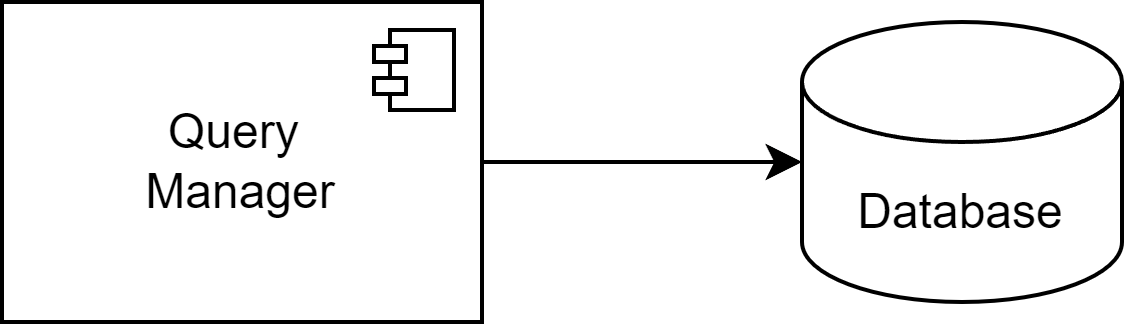
\includegraphics[width=0.5\linewidth]{images/data.png}
        \caption{Representation of the database and query manager}
    \end{figure}
    Now, we can start implementing the components for each user separately. 

    \subsection{Student}
    Due to dependencies between battle and tournament managers of the educator and the notification manager of the student it is better to start the implementation from this last component.
    \begin{figure}[H]
        \centering
        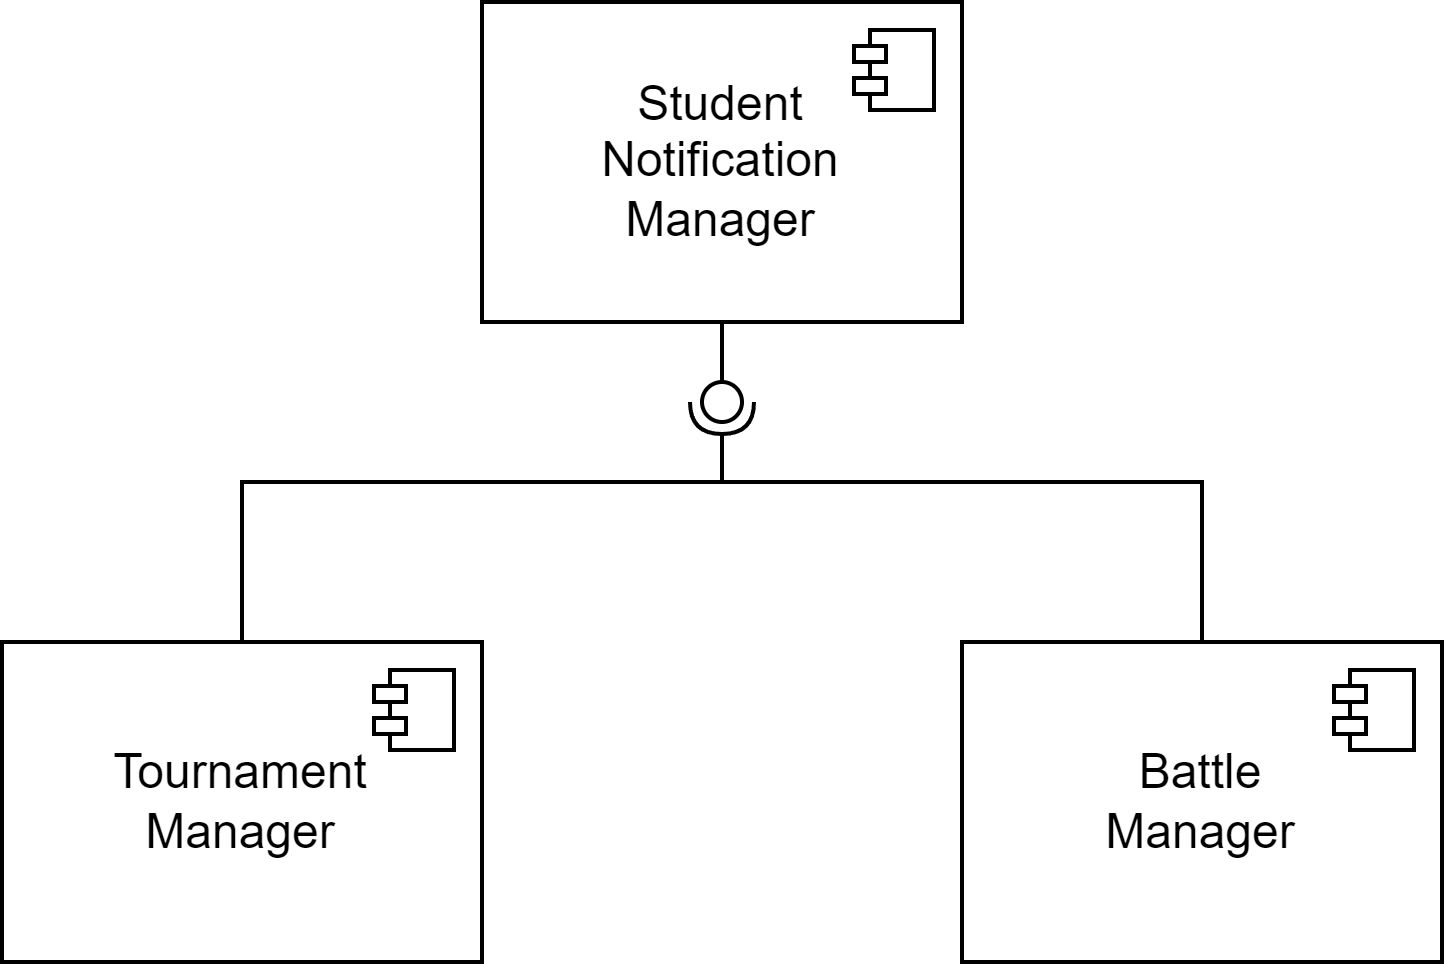
\includegraphics[width=0.5\linewidth]{images/notifications.png}
        \caption{Components that interact to notify the students}
    \end{figure}
    The next component to be developed is the student account manager. 
    The subsequent components to be implemented will be the student research manager with the battle subscription manager and tournament subscription manager. 
    After all these we can finally implement the student profile manager obtaining the complete component that handles all educator functionalities. 
    \begin{figure}[H]
        \centering
        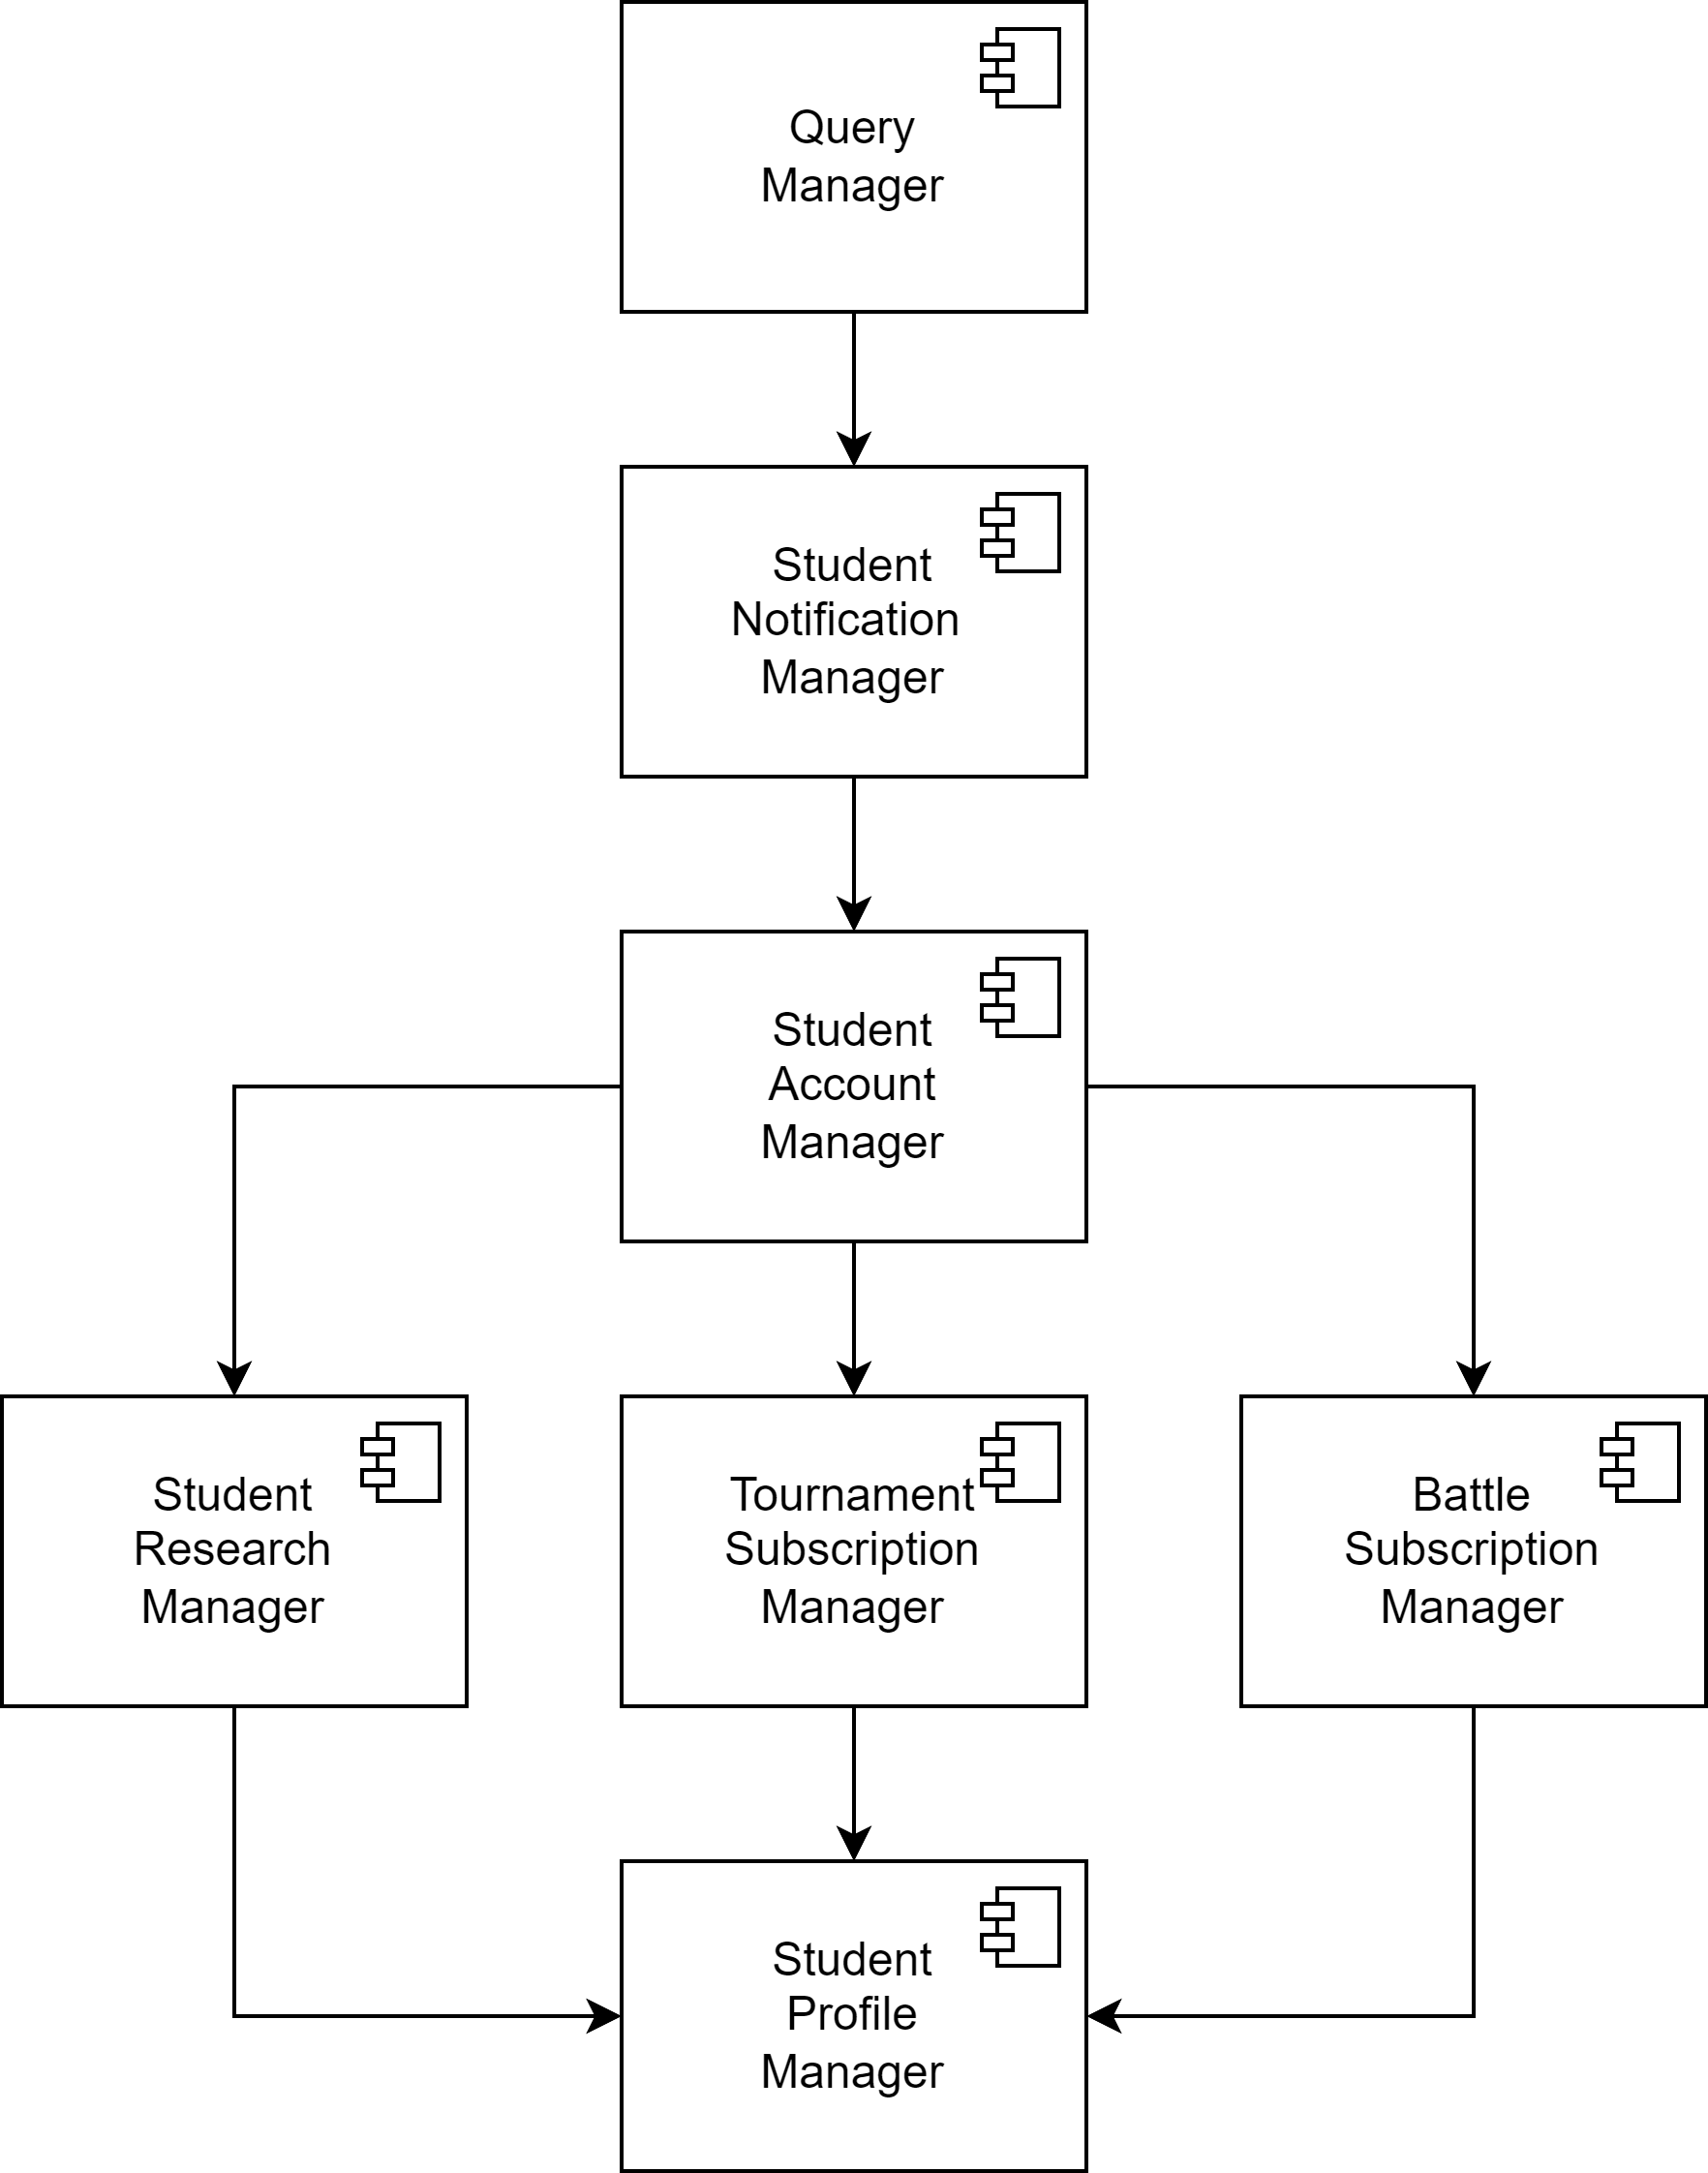
\includegraphics[width=0.5\linewidth]{images/student_impl.png}
        \caption{Implementation order for student manager subcomponents}
    \end{figure}

    \subsection{Educator}
    The educator's component have to be implemented in the same order of the student ones. 
    A diagram that shows the implementation order is shown in the following image
    \begin{figure}[H]
        \centering
        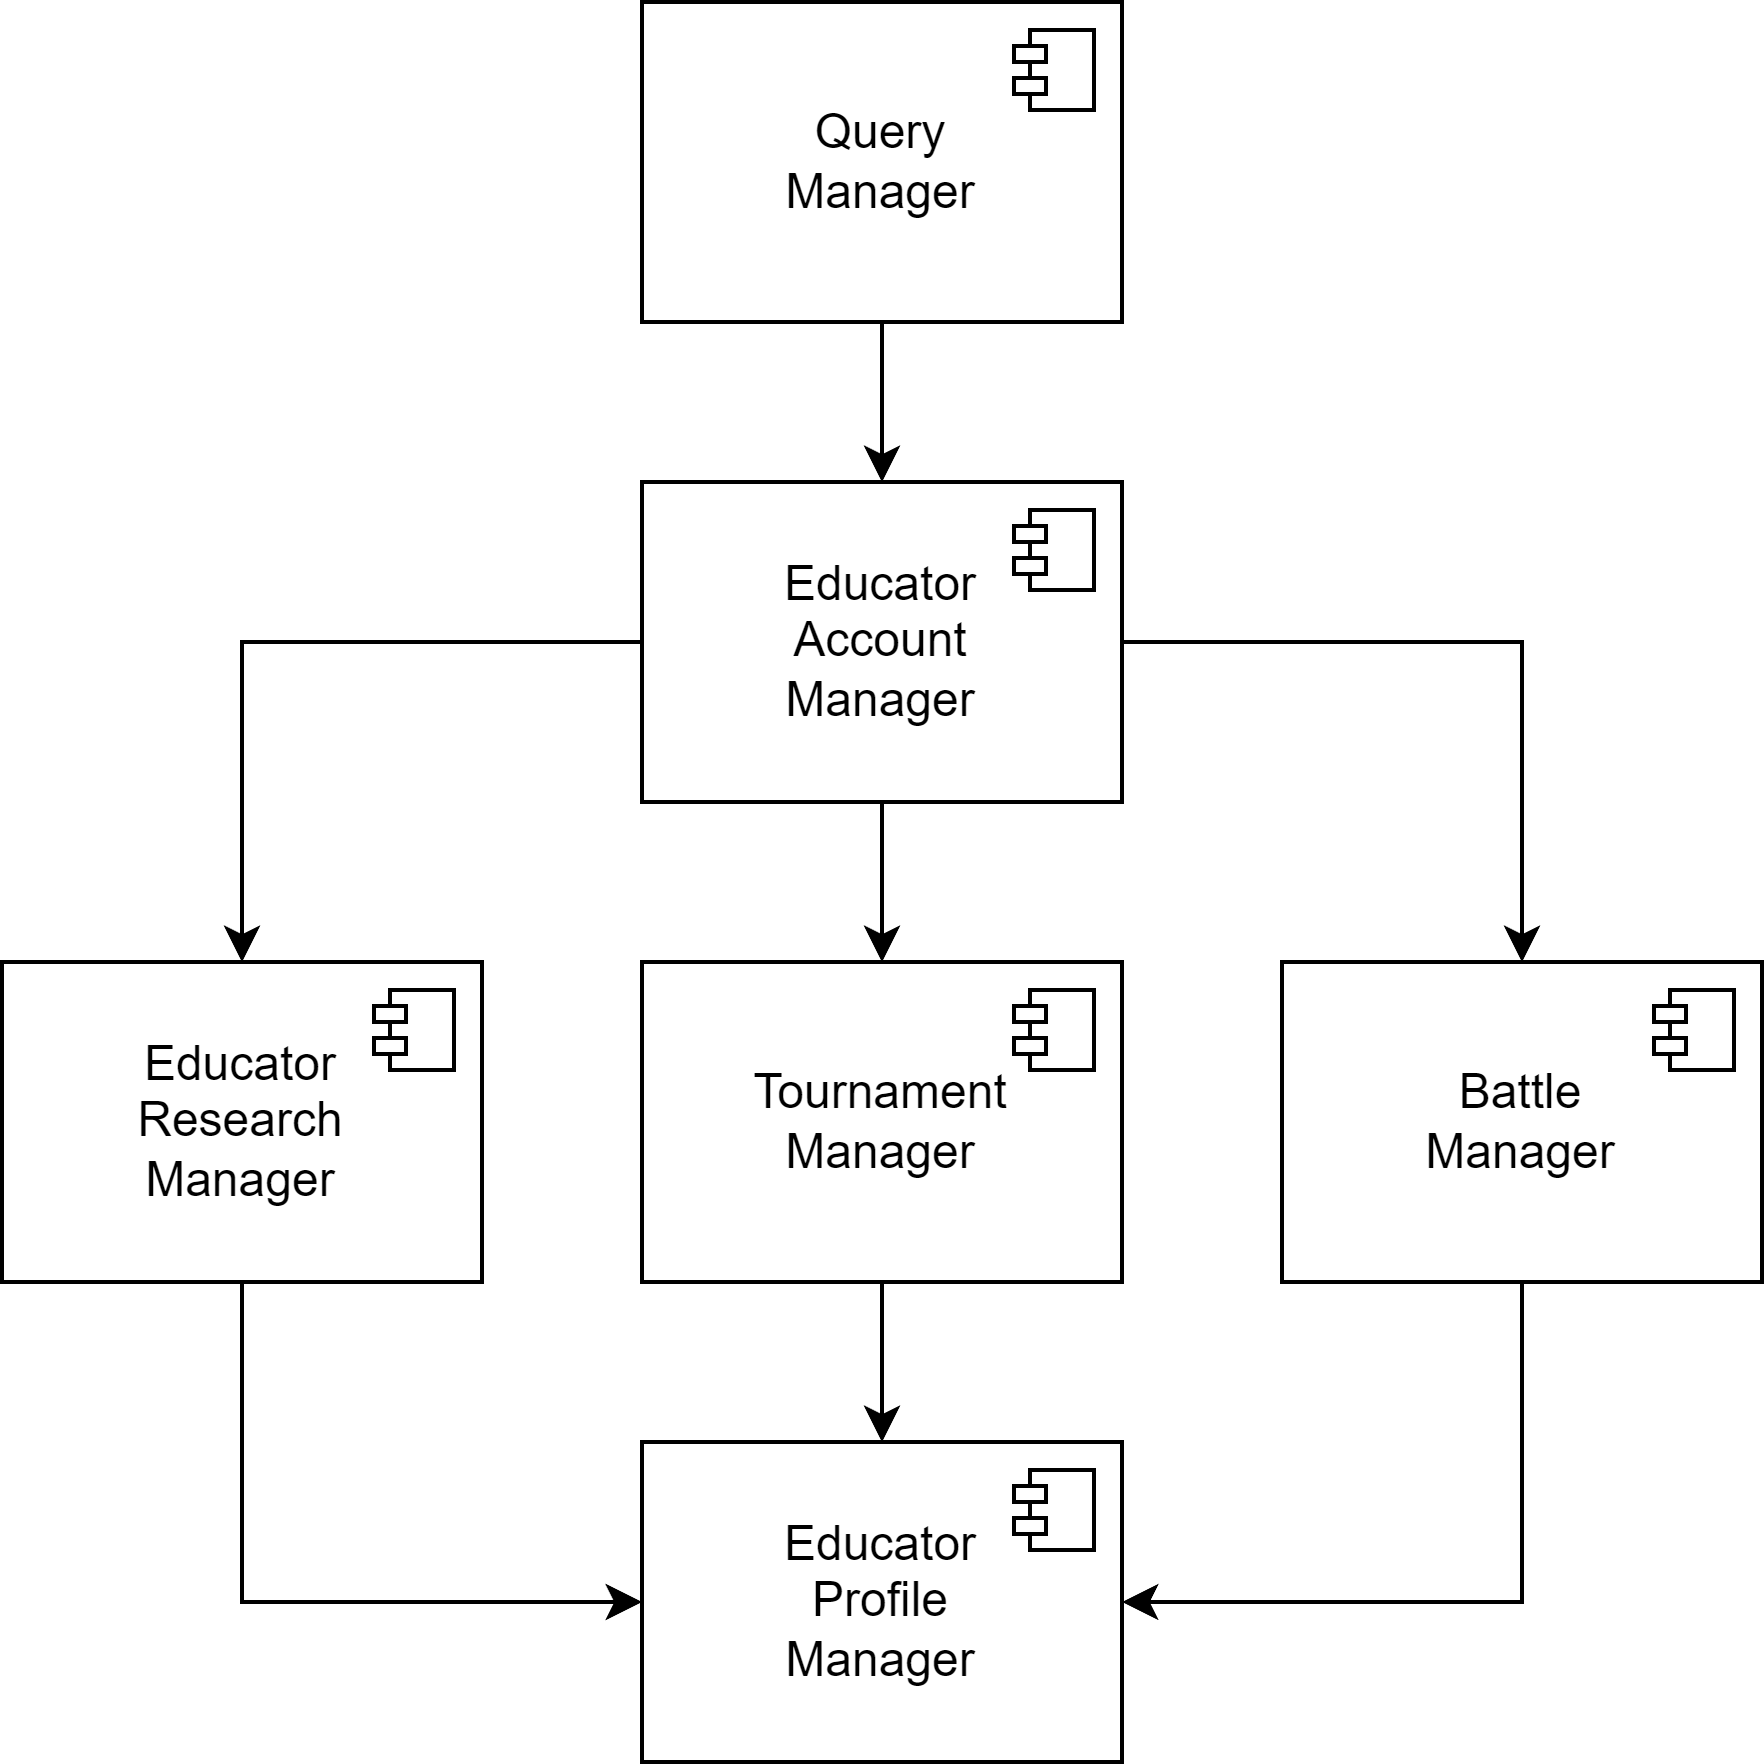
\includegraphics[width=0.5\linewidth]{images/educator_impl.png}
        \caption{Implementation order for student manager subcomponents}
    \end{figure}



    \section{System testing}
    After performing the unit testing on each component the system can be finally integrated. 
    After the integration the testing of the whole system must take place. 
    The objective of this final testing is to check whether the functional and non-functional requirements are met. 
    This testing must be done in a testing environment that is as close as possible to the production environment.
    The CodeKataBattle system needs to undergo the following tests: 
    \begin{itemize}
        \item \textit{Functional testing}: this involves testing the system against the functional requirements and specifications outlined in the Requirements and Specifications Document (RASD).
        \item \textit{Performance testing}: this aims to verify whether a software application remains functional under increased demand and various environmental conditions.
    \end{itemize}

\chapter{Effort spent}
    The table below offers a concise overview of the hours invested by each group member, along with a brief description of their contributions. 
    Dates where the same amount of time was dedicated by all members usually indicates collaborative efforts.
    \begin{table}[H]
        \centering
        \begin{tabular}{cccl}
            \textbf{Date}   & \textbf{Rossi}            & \textbf{Sharoubim}            & \textbf{Description}                          \\ \hline
            20-12-2023      & 2                         & 3                             & First Chapter                                 \\ 
            21-12-2023      & 1                         & 1                             & Overview and component view                   \\ 
            23-12-2023      & 0                         & 3                             & UI Flowcharts                                 \\ 
            27-12-2023      & 4                         & 0                             & Diagrams Component and Deployment View        \\ 
            01-01-2024      & 6                         & 3                             & Runtime View and Architectural Decisions      \\ 
            02-01-2024      & 5                         & 1                             & Interfaces and Testing                        \\ 
            03-01-2024      & 0                         & 2                             & Chapter four                                  \\ 
            04-01-2024      & 2                         & 2                             & Final Revision                                \\ \hline
            \textbf{Total}  & 20                        & 15                            & DD                                            \\  
        \end{tabular}
    \end{table}

\chapter{References}




\end{document}